

\documentclass[12pt]{article}
\usepackage{style}

\title{DL_Book 1_chapter}
\author{М.В. Ронкин, В.В. Зюзин }
\date{г. Екатеринбург, 2021}

\begin{document}
\begin{sloppypar}

\begin{titlepage}
	\centering
% 	\includegraphics[width=0.15\textwidth]{example-image-1x1}\par\vspace{1cm}
	{\scshape ФГАОУ ВО «УрФУ имени первого Президента России Б.Н. Ельцина» или УрФУ \par}
	\vspace{7cm}
	{\huge\bfseries Глубокое обучение систем компьютерного зрения\par}
	{\huge\bfseries Глава 1\par}	
	\vspace{7cm}
	{\Large\itshape Михаил Владимирович Ронкин, Василий Викторович Зюзин, Сергей Владимирович Поршнев \par}
	\vfill  \textsc{г. Екатеринбург, 2021 год.}

	\vfill
	
    \tableofcontents
% Bottom of the page
% 	{\large \today\par}
\end{titlepage}

%%%%%%%%%%%%%%%%%%%%%%%%%%%%%%%%%%%%%%%%%%%%%%%%%%%%%
\newpage
\section{Глава 1. Обзор ретроспективы глубокого обучения сверточных нейронных сетей}
\subsection{Первые теории нейронной сети 1940-1990}
\subsubsection{Модели линейного персептрона средины 20-го века}
Как было сказано \textcolor{red}{во введении} основной подход к решению задач компьютерного зрения на сегодня – это подход на основании глубокого обучения сверточных нейронных сетей. Однако, прежде чем разобраться со сверхточными сетями, следует рассмотреть базовый подход к глубокому обучению – так называемые полносвязные нейронные сети. 

Полносвязные искусственные нейронные сети возникли еще в 1940-е и были вдохновлены гипотезами об устройстве мозга (нейронов в мозге и их связями). Аналогом каждого нейрона было предложена считать \textbf{модель персептрона} (от perceptio – восприятие). Такую модель называют\textbf{ модель МакКаллока-Питтса} 
\cite{mcculloch1943logical}. 
МакКаллоком и Питтсом было предположено, что каждый персептрон, по существу, представляет собой суммирование всех входных данных с регулируемыми весами и взятие какой-либо нелинейной функции от результата этого суммирования. 

    \begin{equation}
    	y = f\left(\sum_{i=0}^{N-1}w_n x_n\right)
    \end{equation}

где $ y $ - результат работы персептрона; $w_n$ - это набор коэффициентов взвешивания каждого входного значения;  $x_n$ - это входные данные; $ f (\cdot )$ - это какая либо нелинейная функция. Часто нелинейная функция называется: \textbf{функция активации}. 
Отметим, что модель МакКаллока-Питтса аналогична работе логистической регрессии. 

Таким  образом можно представить персептрон так, как это показано на рисунке \ref{ch1:fig:1_1}.
    \begin{figure}[!h]
    	\begin{center}
    		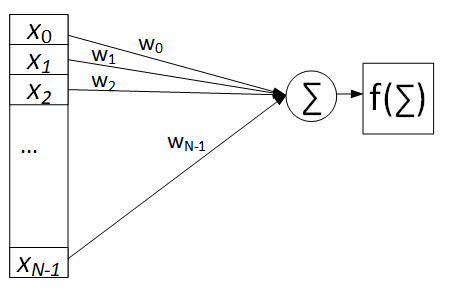
\includegraphics[width=0.5\linewidth]{./figuresch1/perceptron.png}
    		\caption{иллюстрация персептрона}		
    		\label{ch1:fig:1_1}
    	\end{center}
    \end{figure}
В самом общем случае выбор функции активации может быть практически любым. В самых простых случаях, в том числе в модели МакКаллока-Питтса это простая \textbf{ступенчатая функция (пороговая функция)} (1, если $x\geq 0$ 0 или -1 если $x<0$). Однако, на практике к этой функции предъявляется ряд требований, ограничивающих возможности для выбора таких функций. Например, часто полезно, чтобы функция активации имела непрерывную первую производную. 

В отдельных случаях вид функции активации может быть получен аналитически. Так для задачи т.н. бинарной классификации (например, принятия решений о выполнении или не выполнении одной гипотезы, например, есть кошка на изображении или ее нет) – можно получить функцию, называемую сигмоид. Такая функция также часто называется логистической, а соответствующая ей модель персептрона логистической регрессией. Функция сигмоид имеет следующий вид:
    \begin{equation}
    	\sigma(x)= \frac{1}{1+e^{-x}}. 
    	\label{ch1:eqn:sigmoid}
    \end{equation}
В приложении А будет показано как получается такая функция. 
% может записать правило хебба
В оригинальной работе МакКаллока-Питтса не предлагалось конкретного алгоритма обучения - то есть автоматического  подбора весовых параметров. В 1949 году  был предложен алгоритм \textbf{обучение Хебба}  (правила Хебба) для итерационного обучения персептрона вида \ref{ch1:fig:1_1} \cite{hebb1949organization}. Для правил Хебба Новиком позже было доказана сходимость за конечное число шагов (\textbf{теорема Новика}) \cite{novikoff1963convergence}.
Отметим, что термин обучение в случае правил Хебба в означает \textbf{обучение с учителем (supervised learning)}. Сама \textbf{процедура обучения} предполагает автоматический подбор весовых параметров $w_i$ таким образом, чтобы персептрон давал результат с минимальной ошибкой по некоторому критерию, заданному исследователем. Для обучения с учителем предполагается, что есть некоторая обучающая выборка, содержащая набор входные данных и набор результатов для каждого экземпляра (выходных данных, например меток класса (номеров класса) - labels). Тогда \textbf{обучение с учителем состоит} в том, чтобы установить значения весовых параметров $w_i$ так, чтобы средняя ошибка между результатам работы персептрона и ожидаемым результатом (например, меткой класса) была минимальна. 
В случае правил Хебба ошибка рассчитывалась как разность между ожидаемым и полученным ответом. Если ожидаемый ответ был 0, а система давала 1, значения весов нужно было увеличить (чтобы $\sum_i w_ix_i$ стала больше). В обратном случае значения весов нужно было уменьшить. Коэффициент изменения значений весов устанавливался перед обучением \cite{hebb1949organization}. В современном понимании такой коэффициент называется \textbf{скорость обучения (learning rate)}. 

Развитие идей МакКаллока-Питтса и Хебба в технике было предложено в модели \textbf{персептрон Розенблатта}
\cite{rosenblatt1958perceptron, rosenblatt1957perceptron}. 
По существу, предложенное Розенблаттом решение представляет собой полносвязную нейронную сеть с одним скрытым слоем состоящим из одного персептрона - многослойный персептрон. Схема персептрона была впервые реализована аппаратно под названием "Mark 1 Perceptron" схема показана на рисунке \ref{ch1:fig:Rosenblatt}. В данной машине использовался 400 пиксельный сенсор (модуль \textit{S}),  слой проекции на вход персептрона (модуль ассоциации - модуль \textit{А}) и один обучаемый персептрон с 8 выходами типа "да-нет" (модуль \textit{R}, например "да" $+1$, "нет" $-1$). Связи между модулями \textit{S} и \textit{A} устанавливались случайно. Связи в персептроне (связывает модули \textit{A} и \textit{R}) обучались
\cite{hay1960mark}.

\begin{figure}
	\begin{center}
		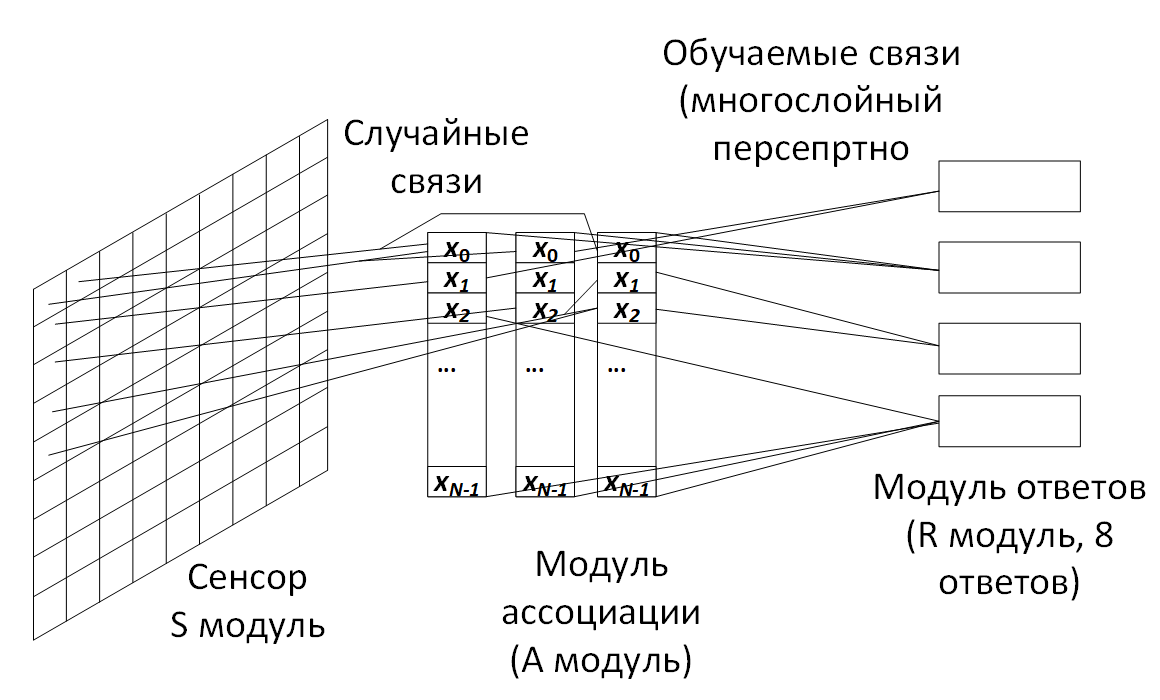
\includegraphics[width=0.7\linewidth]{./figuresch1/Rosenblatt.png}
		\caption{иллюстрация машины "Mark 1 Perceptron", реализующей персептрон Розенблатта}		
		\label{ch1:fig:Rosenblatt}
	\end{center}
\end{figure}

Розенблаттом также была предложена \textbf{итерационная процедура обучения}. В каждой итерации использовался набор  входных данных для каждого из которых был известен результат (тренировочная выборка данных). Таким образом можно было вычислить ошибку, которая могла быть  $0$, $\pm 1$ или $\pm 2$. На каждой итерации все данные подавались в сеть по одному в любом порядке. Итерации продолжались до тех пор, пока сеть не научится выдавать правильные ответы для всех входных примеров. При этом веса персептрона обновлялись после каждого примера, обратно пропорционально полученной ошибке, если ответ был некорректным. 
% разве не правила Хебба!
Таким образом для положительной ошибки веса регулировались для снижения выходного значения, для отрицательного значения ошибки веса повышались. Все обновления значений весов персептрона происходили с предварительно выбранным коэффициентом - известным как \textbf{скорость обучения (learning rate, lr)}. Такой набор правил позже стал известен как правила обучения персептрона \cite{kelleher2019deep}. 
Формально данные правила можно записать следующим образом:

\begin{equation}
	w^{t+1}_i = w^{t}_i+\eta [y^t-\hat{y}^t]x^t_i, 
\end{equation}

где $w^{t+1}_i, w^{t}_i$ - значения весового коэффициента $i$ до и после обновления весов на примере $t$; $y^t-\hat{y}^t$ - ошибка работы персептрона ($y^t$ - целевое значение; $\hat{y}^t$ - результат работы сети); $x^t_i$ - $i$-тый компонент входного воздействия для примера $t$; $\eta$ - предустановленная скорость обучения.

Следует отметить, что в данном случае действует следующий принцип выбора скорости обучения - при слишком низкой скорости обучения изменение средней ошибки по каждой итерации будет незначительным. Если скорость обучения будет слишком высокой, то ошибка по каждой итерации будет как-бы колебаться в положительную и отрицательную стороны, слабо изменяясь в каждой стороне - то есть не будет доходить до минимума. Типичные порядки скорости обучения $0,01 - 0,0001$ в зависимости от задачи. 

В обсуждаемой модели все веса инициализировали случайными значениями. Розенблаттом было доказана \textbf{теорема о сходимости персептрона}. При обучении методом коррекции ошибок персептрон Розенблатта сходится к правильным значениям весов за конечное число итераций независимо от выбора начальных значений весов если допустить, что такой набор весов существует. Под правильными значениями здесь понимается ситуация когда сеть выдает правильные ответы для каждого тренировочного воздействия. Проблемой данного утверждения является то, что обучение может занимать достаточно долго времени и при этом вопрос о существовании "правильного набора весов" будет оставаться открытым. \cite{kelleher2019deep}. 
Практически параллельно Розенблатту была предложена модель персептрона под названием 
\textbf{ADALINE (adaptive linear neuron - адаптивный линейный нейрон)}, 
для обучения которого предлагалось использовать \textbf{метод наименьших квадратов 
(МНК - LMS least mean square)} 
\cite{widrow1960adaptive}. 
Главными отличиями данной модели от модели МакКаллока и Питтса являлись: 
отказ от пороговой функции и процедура обучения персептрона с использованием квадрата ошибки при обновлении значений весов (\textbf{расстояния Евклида, Mean Square Error - MSE}).
Таким образом правило обновления весов можно записать как:

\begin{equation}
	\label{ch1:eqn:ADALINE}
	w^{t+1}_i = w^{t}_i+\eta [y^t-\sum_{i=0}^{N-1}w^{t}_ix^t_i]x^t_i, 
\end{equation}

Для обучения ADALINE использовались те же правила, что и для персептрона Розенблата. 
% разве не правила Хебба!
Однако, в данной нейронной сети обучения могли производится не только с целочисленными ошибками, но и с дробными значениями. Таким образом ADALINE позволяет решать не только задачи бинарной классификации, но и задачи регрессии. В задаче бинарной классификации есть только два ответа ($\pm 1$ или $0-1$). В задаче регрессии необходимо дать ответ в дробных числах. 
\cite{kelleher2019deep}. 
%в непрерывном диапазоне.

Нейронная сеть ADALINE c несколькими персептронами известна как MADALINE  Network. Такая сеть наиболее приближена к современному подходу к архитекторам нейронных сетей. Однако такая сеть была реализована гораздо позже оригинальной работы ADALINE - в силу развития средств вычислительной техники 
\cite{kelleher2019deep}.   

% переписать надо бы 
Основной проблемой, с которой можно столкнуться при наличии только одно персепторна (персептрон МакКаллока-Питтса, Розенблата и ADALINE) является проблема принятия решений в нелинейных ситуациях: это ситуации в которых нельзя одним простым правилом разделить данные на классы (то есть дать правильный ответ или принять правильное решение). Если в задаче можно разделить данные на классы одной линией - то такая задача будет называться \textbf{задача с линейно-разделяемыми признаками (линейная задача)}.\textbf{Линейная задача может быть решена при помощи одного персептрона}. В противном случае будет \textbf{нелинейная задача}. В нелинейной задаче требует более сложная кривая для разделения значений признаков на классы. В нелинейной задаче требуется иметь несколько персептронов прежде чем будет принято решение. Таким образом, \uline{в нелинейной задаче необходимо иметь три слоя: входной, скрытый слой с несколькими персептронами и выходной слой - принятие решений.}
\cite{goodfellow2016deep}.

В самом простом случае нелинейная задача известна как \textbf{\emph{XOR} проблема} (проблема исключающего ИЛИ) 
\cite{minsky1969introduction}.
% проиллюстрировать линейную проблему
Допустим, что есть задача классифицировать автомобили на популярные и непопулярные. При этом для каждого автомобиля есть два признака: цена (разделим на категории - дорого, дешево) и класс (внедорожник или легковой) тогда результаты классификация должна быть такой, как это показано на рисунке \ref{ch1:fig:XOR}. Для того, чтобы разделить автомобили в данном случае потребуется провести две линии (по первому классу и по второму) - таким образом будет два условия для популярного автомобиля: если цена высокая, то класс внедорожник, если цена низкая, то класс легковые автомобили.

\begin{figure} 
	\begin{center}
		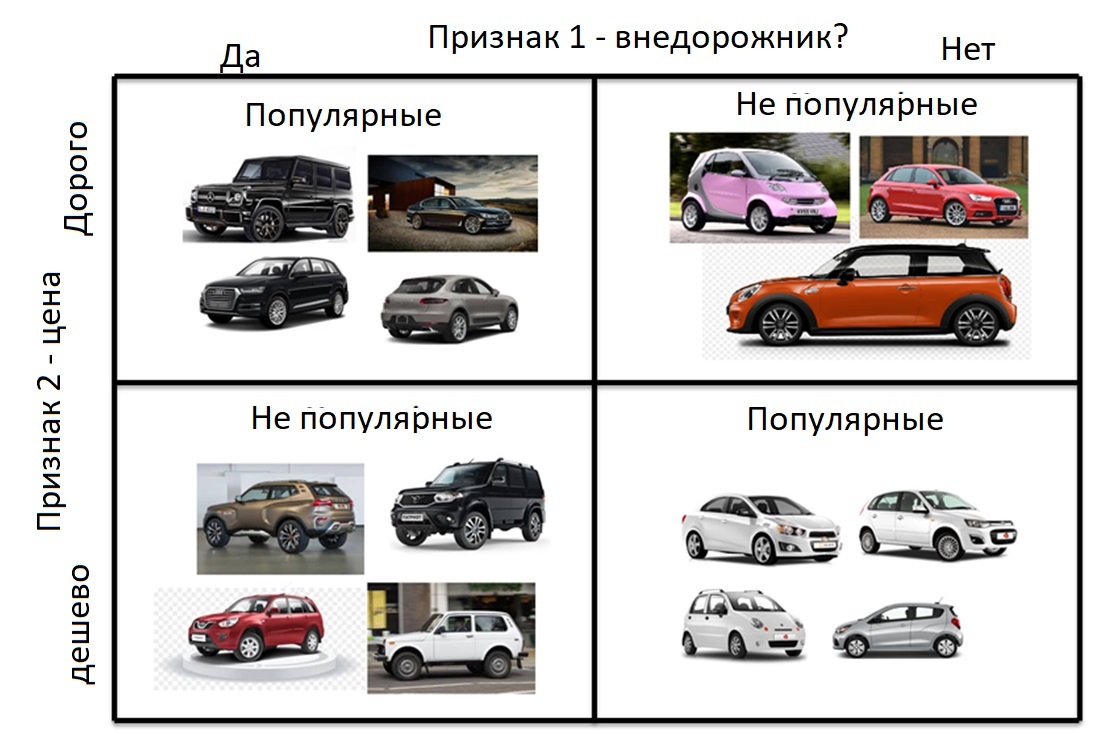
\includegraphics[width=0.7\linewidth]{./figuresch1/XOR_CAR.jpg}
		\caption{иллюстрация XOR проблемы}		
		\label{ch1:fig:XOR}
	\end{center}
\end{figure}

Описанная задача (см. иллюстрацию на рисунке \ref{ch1:fig:XOR}) может показаться элементарной читателю, однако, ее решение недостижимо для любого линейного алгоритма (МакКаллока-Питтса, Розенблата и ADALINE), в том числе одного персептрона. Это объясняется тем, что \textbf{каждый персептрон может провести только одну разделительную линию между признаками}. Фактически это эквивалентно одному условию (например $x>0$). Если нужно провести две линии, как в примере на рисунке \ref{ch1:fig:XOR}, то потребуется два персептрона. 
\uline{
	Обнаружение \emph{XOR} проблемы в 1969 году стало концом первого поколения развития нейронных сетей}.  При этом  большинство ученых перенесли силы в область символьных методов искусственного интеллекта
\cite{goodfellow2016deep}.   

Важно отметить, что окончание перовой волны интереса к нейронным сетями было связано исключительно с уровнем технического развития прогресса. Само по себе решение \emph{XOR} проблемы не представляет трудностей в настоящее время и было реализовано в процессе развития компьютерной техники.
\cite{minsky1969introduction}.

 Пример такого решения с использованием нейронной сети, имеющей один скрытый слой с двумя нейронами показан на рисунке \ref{ch1:fig:XOR_Network}. 

\begin{figure}
	\begin{center}
		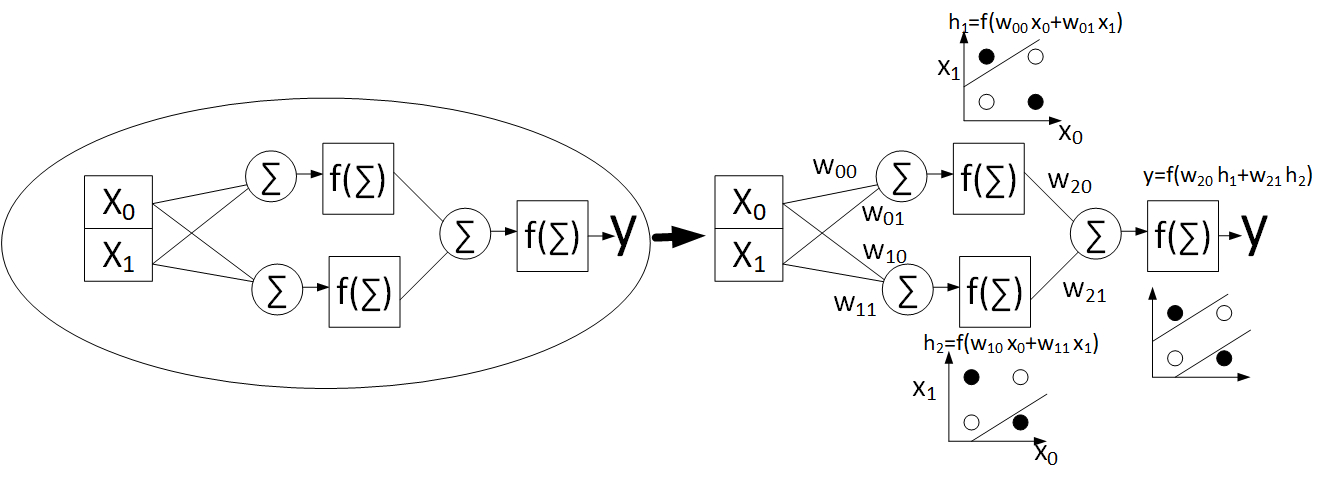
\includegraphics[width=0.9\linewidth]{./figuresch1/XOR_Network.png}
		\caption{иллюстрация нейронной сети для решения XOR проблемы}		
		\label{ch1:fig:XOR_Network}
	\end{center}
\end{figure}

Общее решение таких нелинейных проблем как \emph{XOR} проблемы было предложено советским математиком А.Г. Ивахненко в 1971 г. 
\cite{ivakhnenko1971polynomial}. 
 Предложенный Ивахненко метод группового учета данных (GMDH, group method of data handling) является одними и обсуждаемых методов для реализации в современных глубоких нейронных сетях
\cite{schmidhuber2015deep, kelleher2019deep}. 

Отметим также, что строго говоря термин "линия" применим к двух-мерному рассмотрению задачи. 
Двухмерная задача - это когда рассматривается два признака, например, один по оси абсцисс (скажем x), другой по оси ординат (скажем, y). В более общем случае - когда признаков больше аналогом линии становится \textbf{гиперплоскость} (в случае с тремя признаками просто плоскость). Также следует отметить, что такое абстрактное представление пространства образованного признаками называется  \textbf{признаковое пространство}. 

\subsubsection{ Многослойный персептрон Румельхарта 1980-е}
%%%%%%%%%%%%% RUMELHART %%%%%%%%%%%%%%%%%%%%%

Идея использования большого количества нейронов объединенных вместе в многослойную нейронную сеть была развита в первой половине 1980-х (\textbf{идея коннекционизма}). Технически основание коннекционизма лежит в развитие распределенных систем параллельной обработки данных. Также идеей коннекционизма является идея представления данных в виде набора признаков и формирование каждого выхода нейронной сети принимая во внимание все входные признаки 
\cite{goodfellow2016deep}. 
Идеи коннекционизма были развиты группой 
PDP (parallel distributed processing, параллельная распределенная обработка) во главе с Д.Е. Румельхартом. Данной группой в 1985-1986 были предложены архитектура нейронной сети - \textbf{многослойный персептрон  Румельхарта}
\cite{rummelhart1986parallel}
и метод обучения многослойного персептрона -\textbf{ метод обратного распространения ошибки (backpropagation)} 
\cite{rumelhart1985learning} (авторы Rumelhart D.E., Hinton G.E., Williams R.J.). Также важно отметить, что метод обратного распространения ошибки предлагался много раз до 1985 г., однако популярность приобрел только после публикации \cite{rumelhart1985learning}. В частности, метод предлагался в работе советского математика А.И. Галушкина, посвященной многослойным системам распознавания образов \cite{Galushkin1974synthesis}. Также метод обратного распространения ошибки был независимо предложен Барцевым С. И., Охониным В. А. в 1985 г \cite{Barcev1986adaptive}.  Архитектура нейронной сети - персептрон Румельхарта  часто называется \textbf{многослойный персептрон - Multilayer Perceptronб MLP} или \textbf{полносвязная нейронная сеть (Full-Connected Neural Netwrok, FCNN)}. Иллюстрация FCNN архитектуры приведена на рисунке \ref{ch1:fig:MLP_Arch}.

\begin{figure}
	\begin{center}
		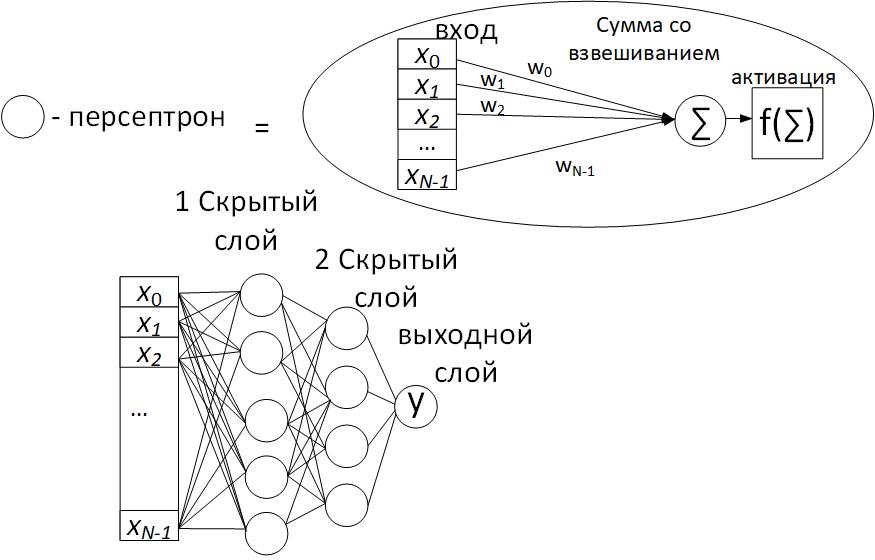
\includegraphics[width=0.8\linewidth]{./figuresch1/MLP_Arch.png}
		\caption{иллюстрация многослойного персептрона}		
		\label{ch1:fig:MLP_Arch}
	\end{center}
\end{figure}

Отдельно следует остановиться на методе обратного распространения ошибок. Данный метод обучения многослойного персептрона наиболее популярный и лежит в основе обучения современных глубоких нейронных сетей. В том числе сверточных нейронных сетей. Математическим аспекты вариантов реализации данного метода будут рассмотренных в соответствующих разделах данной книги. Однако, тут следует также пояснить суть данного метода "на пальцах". 

В основе метода обратного распространения ошибки лежит метод градиентного спуска. На самом деле частный случай данного выражения уже был приведен \ref{ch1:eqn:ADALINE} для ADALINE персептрона. Суть метода заключается в обновлении значений весов нейронной сети обратно пропорционально ошибки - почти как правила обучения Хебба, но для работы с 
\textcolor{red}{дробными значениями}. 
Вывод выражения для градиентного спуска приведен в 
\textcolor{red}{приложении А}.

Рассмотрим идею градиентного спуска более подробно.
В самом простом случае градиент это производная. 
Допустим, что ошибка предсказания нейронной сети как средне-квадратичная ошибка:

\begin{equation}
	\label{ch1:eqn:MSELoss_ch1}
	err_i = L(y_i,\hat y_i) = (y_i - f(\sum_{j=0}^{N-1}w_jx_{ij}))^2 = (y_i - f(W^TX_i))^2,
\end{equation}
где:
\begin{itemize}
    \item $err_i$ - средне-квадратичная ошибка для примера $i$. Такую ошибку принято называть \textbf{функция потерь (loss function)}.
    \item $L(y_i,\hat y_i)$ - обозначение функции потерь как функции от ожидаемого результата $y_i$ и полученного $\hat y_i$. Таким образом \uline{функция потерь это и есть некоторая мера сравнения ожидаемого и полученного результатов}. Мера может быть выбрана практически любой. Однако, когда речь идет об ошибки - подразумевается, что мера имеет нулевое значение, когда $y_i$ и $\hat y_i$  равны друг другу.
    \item $W = {w_0,w_1,...,w_j,...w_{N-1}}$ - вектор весовых параметров.
    \item $X = {x_0,x_1,...,x_j,...x_{N-1}}$ - вектор входных параметров (например признаков для одного экземпляра данных). \\ Отметим также, что $\sum_{j=0}^{N-1}w_jx_{ij} \equiv W^TX_i$ по определению скалярного произведения векторов.
    \item $f(\cdot)$ - некоторая функция активации.
\end{itemize}

 Набор производных $L(y_i,\hat y_i)$ по всем $w_j$ - будет называться \textbf{градиент функции} в данном случае
 \underline{случае градиент функции потерь}: 

 \begin{equation}
	\label{ch1:eqn:nablaL}
	 \nabla L = \left\{
	 \frac{\partial L}{w_0},
	 \frac{\partial L}{w_1},
	 ...,
	 \frac{\partial L}{w_j},
	 ...,
	 \frac{\partial L}{w_{N-1}}
	 \right\}
\end{equation}

 Направление градиента будет направлением роста функции, а модуль градиента покажет скорость роста функции. Таким образом для достижения минимума функции потерь требуется следующее.
 
 \begin{itemize}
 \item Определить выражение $\nabla L$ (\ref{ch1:eqn:nablaL}) - это покажет направление изменения значений в сторону роста функции потерь. 
  \item Изменить значения веса в обратную сторону. 
 \item Коэффициент изменения значений весов будет называть \textbf{скорость обучения.}  Выбор скорости обучения очень важен, о чем писалось выше. Легко представить себе ситуацию когда из-за слишком большой скорости обучения значения оптимальных весов будут пропущены.
\end{itemize}

Общее выражение для обновления весов

\begin{equation}
	\label{ch1:eqn:GradDescent}
	W^{\{t+1\}} = W^{\{t\}} - \eta \nabla L(\hat y^{\{t+1\}},y^{\{t+1\}}),
\end{equation}

где $W^{\{t+1\}}, W^{\{t\}}$  - значения весов на шаге обучения $t+1$ и $t$ соответственно; $\hat y^{\{t+1\}} = (W^{\{t\}})^TX^{\{t+1\}} , y^{\{t+1\}}$ - значения входных и выходных данных для шага $t+1$; $L(\cdot)$ - функция потерь; $\nabla L$ - градиент функции потерь; $\eta$ - скорость обучения. 

В выражении \ref{ch1:eqn:GradDescent} функция потерь может быть любой, для которой существует первая производная. При этом нет необходимости в аналитическом расчете  значений $\nabla L$, процедура расчета значений градиента выполняется исключительно численными методами
\cite{Nikolenko2017DL}.

Для иллюстрации принципа работы градиентного спуска рассмотрим функцию одной переменной $err(w)$ вида (\ref{ch1:eqn:MSELoss_ch1}). Для такой функции потерь производная по $w$ будет иметь вид 

\begin{equation}
\frac{\partial err(w)}{\partial w} = \frac{\partial (y_i-wx_i)^2}{\partial w}= 2(y_i-wx_i)x_i.
\end{equation}

Иллюстрация для такого вида функции потерь и ее градиента показан на рисунке \ref{ch1:fig:MSELoss_1_variable}. На рисунке показано, что скорость изменения значения функции потерь снижается с приближением к ее минимальному значению $err_{min}$. Минимальному значению функции потерь соответствует оптимальное значение веса $w^*$. Направление изменения весов к $w^*$ - называется \textbf{направление градиентного спуска} или  направление антиградиента.

\begin{figure}
    \begin{center}
		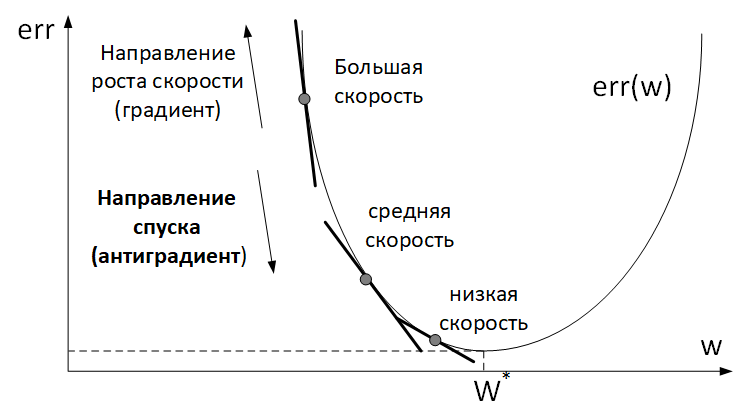
\includegraphics[width=0.8\linewidth]{./figuresch1/MSELoss_1_variable.png}
		\caption{иллюстрация функции потерь $err$ для одного параметра $w$ и ее градиента.}		
		\label{ch1:fig:MSELoss_1_variable}
	\end{center}	
\end{figure}

Метод градиентного спуска относится к методам оптимизации. Существует достаточно много модификаций метода, в том числе позволяющих избежать проблему выбора скорости обучения. Однако, не все они применимы к обучению нейронных сетей. Позже наиболее популярные модификации методов градиентного спуска будут рассмотрены в приложении к глубокому обучению.

Отметим, что задача градиентного спуска характерна для многих приложений регрессии. В том числе данным методом может быть решена и задача логистической регрессии. Кроме того следует отметить, что для случая линейной регрессии задача оптимизации решается в явном виде - в закрытой форме, то есть в виде аналитического выражения. Однако, если параметров в регрессии достаточно много, то также рекомендуется использовать метод градиентного спуска.

\textit{
В случае когда обучению подлежит многослойный персептрон метод градиентного спуска в своей прямой реализации становится достаточно сложным с вычислительной точки зрения.
} 

Рассмотрим персептрон Румельхарта с одним скрытым слоем. Для такой нейронной сети есть два набора весовых параметров (первый набор: вход - скрытый слой и второй набор: скрытый слой - выход). расчет градиента для первого набора - потребует расчет вектора весов. Расчет градиента для второго слоя потребует расчета матрицы и т.д. Однако процедура может быть упрощена если представить что каждый слой (скрытый и выходной) независимы. Тогда отдельно можно представить скрытый слой как персептрон с большим количеством выходов и отдельно выходной слой, для которого выход скрытого слоя будет входными данными. В этом случае значение функции потерь на выходе нейронной сети можно пересчитать на скрытый слой и обновить значения весов по каждому слою отдельно. Данная идея лежит в основе метода обратного распространения ошибки. 

\uline{Формально метод  обратного распространения ошибки может быть записана следующим образом, для многослойного персептрона с $K$ слоями ($k=0,...,K$, $k=0$ - вход) для $k>0$}:

\begin{equation}
\label{ch1:eqn:backpropagation}
\begin{cases}
     W_{k}^{\{t+1\}} = W_{k}^{\{t\}}-\eta \frac{1}{m_k}\frac{\partial L }{\partial W_{k}};
     \\\\
    \frac{\partial L }{\partial W_{k}}= \left(e_{k} \odot \frac{\partial f(z_{k})}{\partial z_{k} } \right)  O_{k-1}^T; 
    \\\\
    e_{k} = e_{k+1}\left(\big[W_{k+1}^{\{t\}}\big]^T\odot \frac{\partial f(z_{k+1})}{\partial z_{k} }\right), \text{ $1\le k < K$};
    \\\\
    e_{K} = \frac{\partial L }{\partial \hat y};
 \end{cases},
\end{equation}
где
\begin{itemize}
\item $W_{k}^{\{t+1\}} , W_{k}^{\{t\}}$ - значения вектора весов для слоя с номером $k$ на шаге обучения $t+1$; 
\item $m_k$ - число входных параметров для слоя с номером $k$;
\item $\eta$ - коэффициент скорости обучения; 
\item $e_{k}$ - значение ошибки для слоя с номером $k$; 
\item $z_k =  (W_{k}^{\{t\}})^T O_{k-1}$; 
\item $O_{k-1}$ - выход  $k-1$ слоя (вход слоя $k$);
\item $\frac{\partial f(z_{k})}{\partial z_{k}}$ - производная функции активации.
\end{itemize}

Таким образом, 
\uline{алгоритм  вычисления значений обновлений весовых параметров многослойной нейронной сети методом обратного распространения ошибки} 
следующий \cite{Nikolenko2017DL}. 

 \begin{itemize}
    \item На каждом шаге ее обучения повторить две стадии: прямое и обратное распространение.
 	\item Прямое распространение (forward propagation), при котором на вход подаются данные и получается ответ на выходе.
 	\item Обратное распространение (backward propagation), при котором происходит:
 	   \begin{itemize}
     	  \item расчет ошибки работы нейронной сети и ее градиента, 
     	  \item пересчет градиента функции ошибки на результат для каждого слоя (пропорционально значениям весов с которыми учтен каждый нейрон).
     	  \item обновление значений весов для каждого слоя в соответствие суммарным градиентом ошибки его работы.
 	   \end{itemize}
 \end{itemize}
Отметим, что в основе использования метода обратного распространения ошибки лежит т.н. 
\textbf{правило цепочного дифференцирования}. 
По существу, метода обратного распространения ошибки, является всего лишь 
\textcolor{red}{вычислительным представлением данного правила}. 
Для запуска алгоритма обратного распространения ошибки необходимо про-инициализировать значения всех весовых параметров нейронной сети некоторыми случайными значениями. Каждая итерация в алгоритме обратного распространения ошибки называется \textbf{эпоха}. 
Число эпох может быть задано из некоторых априорных соображений (опыта). Однако, чаще всего обучения прерывают по некоторому условию. Типичные условия для остановки процедуры обучения нейронных сетей будут рассмотрены в книге далее.  

Одним из ключевых требований к использованию метода обратного распространения ошибок является требование существование производных функций активации и функции потерь. В моделях персептрона первой волны (МакКаллок-Питтс и Розенблатт) как правило использовалась пороговая функция активации. Однако, пороговая функция не могла быть использована с методом обратного распространения ошибок. Пороговую функцию можно заменить на логистическую или на гиперболический тангенс. Другие, менее тривиальные требования к методу  обратного распространения ошибок будут рассмотрены позднее. 

Важно отметить, что в многослойном персептроне, как правило, вид функции потерь будет отличаться от показанного на рисунке 
\ref{ch1:fig:MSELoss_1_variable}, 
и будет иметь ряд локальных минимумов помимо одного глобального. Задачи, когда имеется только один минимум (\textbf{глобальный минимум}) 
называются задачами выпуклой оптимизации.
\uline{ В нейронных сетях рассматриваются задачи не выпуклой оптимизации, когда имеется ряд локальных минимумов и один глобальный.} Другими словами 
\textbf{ландшафт функции потерь} может быть как выпуклым, так и не выпуклым. Пример не выпуклого ландшафта  функции потерь показана на рисунке 
\ref{ch1:fig:Non_Convex_1var}. 
В пределе число локальных минимумов может быть равно числу нейронов. Возникающие при этом проблемы связаны с тем, как избежать попадания в локальные минимумы и тем, как не пропустить глобальный минимум.   
\cite{Nikolenko2017DL}.  Отметим, что в ряде работ, в том числе \cite{lecun1998gradient} утверждается, что вероятность попадания в локальный минимум при градиентном спуске снижается с ростом числа параметров в нейронной сети (в случае если число параметров нейронной сети больше чем необходимое число признаков для однозначного решения задачи) \cite{lecun1998gradient}. 

 \begin{figure}[h]
 	\begin{center}
 		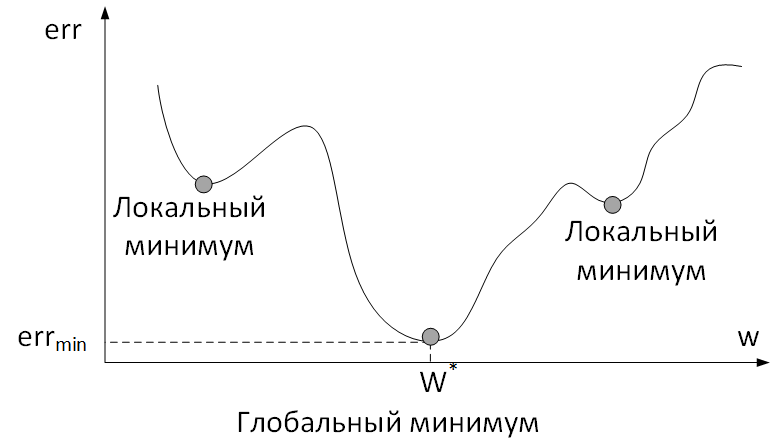
\includegraphics[width=0.7\linewidth]{./figuresch1/Non_Convex_1var.png}
 		\caption{иллюстрация типичного ландшафта функции потерь многослойного персептрона в двухмерной плоскости}		
 		\label{ch1:fig:Non_Convex_1var}
 	\end{center}
 \end{figure}

% TODO: уточнить формулировку, ссылку на граф
С точки зрения концепции параллельных распределенных вычислений удобно представить многослойный персептрон в виде вычислительного графа. 
\cite{Nikolenko2017DL}.
\textbf{Вычислительный граф} - это разбиение сложной процедуры вычислений на элементарные операции. Каждая операция представляет собой узел графа. Пример такой процедуры для многослойного персептрона с одним скрытым слоем проиллюстрирован на рисунке \ref{ch1:fig:comp_gpraph}. 
 
 \begin{figure}[!h]
 	\begin{center}
 		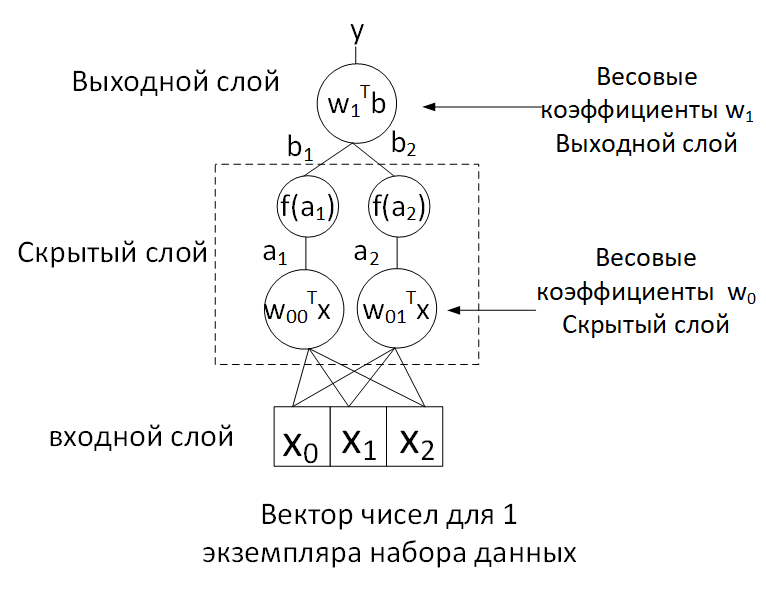
\includegraphics[width=0.7\linewidth]{./figuresch1/comp_gpraph.png}
 		\caption{иллюстрация вычислительного графа, $w^Tx = \sum wx$}		
 		\label{ch1:fig:comp_gpraph}
 	\end{center}
 \end{figure}

% TODO: уточнить формулировку, ссылку на граф
При использовании такого подхода метод обратного распространения ошибки может быть сведен к вычислению производных по каждому ребру графа - что позволяет легко проводить вычисления, необходимые для обучения нейронной сети на любых устройствах, позволяющих распараллеливание операций. 
\cite{Nikolenko2017DL}. 

\subsubsection{Фундаментальные основы функционироания нейронных сетей 70-е - 90-е}
%%%%%%%%%%%%%%%%%%%%%%%%%% ЦЫБЕНКО %%%%%%%%%%%%%%%%%
% СНАЧАЛА ВАПНИК ТОГДА
% Лема Уитсона!
% надо разобраться емкость алгоритма это число параметров или нейронов?
по ссылкам ниже про Вапника и обобщающую способность
% https://mjt.cs.illinois.edu/dlt/#vc-dimension-of-linear-predictors
% https://arxiv.org/pdf/2012.05760.pdf
В 1989 г. Джоржем Цыбенко была доказана универсальная теорема аппроксимации - утверждающая, что достаточно плоносвязной нейронной сети с одним скрытым слоем для аппроксимации любой функции  и с любой точностью (зависящей от числа нейронов в скрытом слое). При этом сеть должна иметь вид 
\cite{cybenko1989approximation}:

\begin{equation}
\label{ch1:eqn:Cybenko}
\hat y = \sum_{j=0}^{N-1} {w_{1j} f(\sum_{i=0}^{M-1} w_{ij} x_i + \theta_j) },
\end{equation}

где $\hat y$ - результат аппроксимации; 
$\{x_i\}_{i=0}^{M-1}$ - набор входных данных (вектор $M$ признаков для одного экземпляра); 
$ \{ w_{1j} \}_{j=0}^{N-1}$ - набор (вектор) весов скрытого слоя ($N$ нейронов); 
$\{ \theta_j \}_{j=0}^{N-1}$ - набор смещений входных данных для скрытого слоя (вектор из $N$ смещений); 
$\{ w_{ij} \}_{i,j=0}^{M-1,N-1}$ - двухмерный набор весов для входного слоя; 
$f(\cdot)$ - функция активации, такая, что $f(z)\to 1$ если $z \to \infty$ и $f(z)\to 0$ если $z \to -\infty$, например логистическая функция ($f(z) = 1/[1+exp(-z)]$).

В 1991 Куртом Хроником  результат \ref{ch1:eqn:Cybenko} был обобщен на случай произвольной дифференцируемой функции активации \cite{hornik1991approximation}. Также рядом авторов были приведены доказательства универсальная теорема аппроксимации для других частных случаев архитектур полносвязных нейронных сетей, в том числе многослойных нейронных сетей \cite{kidger2020universal} и нейронных сетей с т.н. остаточными связями \cite {tabuada2020universal} (данный тип связей будет подробно рассмотрен и объяснен в книге далее). Также следует отметить, что результат \ref{ch1:eqn:Cybenko} основан на теореме Колмогорва-Арнольда (1956, 1957 гг), которая утверждает, что функцию многих переменных можно представить в виде набора функций одной переменной, как \cite{Arnold1957variables3, Kolmogorov1957representation}:

\begin{equation}
\label{ch1:eqn:Kolmogorv_Arnold}
\hat y(x_0,...,x_{M-1}) = \sum_{j=0}^{2M} F_j(\sum_{i=0}^{M-1}G_{ij}(x_i)) ,
\end{equation}
где $F_j(\cdot) и G_{ij}(\cdot)$ - наборы некоторых функций одной переменной; $y(x_0,...,x_{M-1})$ - функция $M$ переменных. 

\textcolor{red}{Важным следствием результата \ref{ch1:eqn:Kolmogorv_Arnold} является наличие в нейронной сети с одним скрытым слоем, в котором не менее чем $2M+1$ нелинейных узлов (нейронов) для $M$ признаков, описывающих данные. При этом, интуитивно понятно, что тут речь идет о независимых признаках - то есть признаках не коррелирующих (не связанных) друг с другом. Только в этом случае данные образуют  $M$-мерное признаковое пространство. Если два признака во входных данных будут иметь одинаковое поведение, то задача будет недоопределенной. }
 
Другим следствием результата \ref{ch1:eqn:Kolmogorv_Arnold} является то, что решение задачи для $M$ признаков требует не менее, чем $(2M+1)\cdot M \approx 2M^2$ параметров для полносвязной нейронной сети. 
\textcolor{brown}{Также интуитивно понятно, что для вычисления $(2M+1)\cdot M$ параметров необходимо иметь не менее, чем $(2M+1)\cdot M$ экземпляров данных. Это следует из аналогии с системами уравнений, в том числе с системами линейных уравнений. При этом речь идет о данных в которых каждый признак представлен независимо. Например, если стоит задача отличить кошек от собак - то надо взять $(2M+1)\cdot M/2$ как можно более разных фотографий собак и столько же кошек. Если есть вероятность, что часть данных тренировочной выборки коррелирует, то выборку надо увеличить. На практике такая вероятность есть всегда, поэтому выборку надо брать предельно большой или использовать специальные меры по регуляризации решения \textcolor{purple}{слабоопределенных} задачи. Позже в книге будут рассмотрены методы регуляризации обучения, характерные для компьютерного зрения. } 

Отметим также, что требования по наличию $2M+1$ параметров в скрытом слое и $M$ параметров во входном слое для задачи требующей $M$ следует из теории Вапника-Червоненкиса (советские математики, 1971 г.) \cite{vapnik1971uniform}. 
Авторами было введено понятие размерности Вапника-Червоненкиса. Данная размерность показывает максимальное число способов классификации (разделения) данных.  Для линейных систем составляет $M+1$ гиперплоскостей. Для нелинейных систем типа многогранник размерность составляет $2M+1$. 
% Необходимо где то уточнить все или я правильно понимаю из того что описано ниже 
\textcolor{red}{
Таким образом, если есть есть $M$ экземпляров данных для которых выделено $M$ признаков - то такая задача классификации решается линейной системой. В этом случае остается, например,  перебрать возможные способы классификации и выбрать лучший. Если для решения задачи необходимо $2M+1$ признаков, то задача должны решаться нелинейным классификатором.
% Особенно то что тут написано
% http://www.machinelearning.ru/wiki/index.php?title=%D0%A0%D0%B0%D0%B7%D0%BC%D0%B5%D1%80%D0%BD%D0%BE%D1%81%D1%82%D1%8C_%D0%92%D0%B0%D0%BF%D0%BD%D0%B8%D0%BA%D0%B0-%D0%A7%D0%B5%D1%80%D0%B2%D0%BE%D0%BD%D0%B5%D0%BD%D0%BA%D0%B8%D1%81%D0%B0
Если необходимо более чем $2M+1$ - задача не имеет однозначного решения для обсуждаемых условий. 
Таким образом в случае архитектуры нейронной сети, соответствующей выражению (\ref{ch1:eqn:Cybenko}) необходимо взять $M$ линейных персептронов и построить многоугольник из гиперплоскостей, затем на данном многоугольнике необходимо выбрать классификатор из $2M+1$ вариантов. }
\textcolor{brown}{
ОТСЮДА УЖЕ ДОЛЖЕН ИДТИ ЦЫБЕНКО - ЧТО ЭТОГО ДОСТАТОЧНО. ВАПНИК - НЕОБХОДИМО, ЦЫБЕНКО ДОСТАТОЧНО}.

Также следует отметить, что в ряде работ, в частности,  \cite{vapnik1982estimation, vapnik1994measuring} 
было показано, что чем больше размерность Вапника-Червоненкиса тем больше данных требуется для обучения алгоритма и тем выше потенциальная обобщающая способность алгоритма. Кроме того для фиксированного размера тренировочной выборки разность ошибок на тестовых и на тренировочных данных будет выше для алгоритма с большей размерностью. 

\textcolor{brown}{
Также Вапником было показано для каждой задачи может существовать оптимальная размерность с точки зрения выше описанных свойств \cite{vapnik1974recognition}
% http://www.ccas.ru/voron/download/Generalization.pdf
}

\textcolor{brown}{
также из анализа разности ошибок на обучение и тесте следует условие оптимального обучения - то есть ситуация когда разность таких ошибок минимально. В других случаях речь идет о переобученности.
}

\textcolor{brown}{
Из теории Вапника также следует, что чем больше тренировочная выборка и чем больше размерность алгоритма (его емкость), тем меньше ошибка на тренировочной выборке. То есть потенциально и тем меньше ошибка на тестовой выборке - то есть тем больше обобщающая способность.
}

\textcolor{brown}{
Также надо отметить, что из размерности Вапника-Червоненкиса следует, например, что XOR проблема не решается линейным алгоритмом, но решается нелинейным (для 2 признаков размерность 3 для лин. алго и 5 для нелин.). 
}

\textcolor{brown}{
Размерность нелинейного алго можно повысить!? она растет полиномиально?!
Принцип минимизации сруктурного риска!?
}

\textcolor{brown}{
Как правило, в задачах компьютерного зрения не удается выделить (формализовать, описать) все необходимые признаки для ее решения. Например, достаточно сложным будет выделить все необходимые признаки для распознавания лица человека на изображении с произвольного ракурса. Таким образом проблема определения числа необходимых параметров нейронной сети и проблема размера выборки данных для обучения остается открытом вопросом.  Однако, в пределе можно сказать, что число признаков равно размеру каждого экземпляра данных, например изображение размером $320\times 240$ предельно будет содержать $76 800$ признаков, хотя на само деле их скорее всего будет меньше, но сколько определить нельзя. При этом, нейронная сеть вида \ref{ch1:eqn:Cybenko} 
для такого количества признаков потребует наличие $\sim 12$ миллиардов параметров и столько же входных данных - что является достаточно большой цифрой даже для современной вычислительной техники (2021 год). Поэтому требует каких-либо использование методов снижения числа параметров. 
\uline{Проблема снижения числа параметров нейронной сети приводит в задачах компьютерного зрения к использованию сверточных нейронных сетей, изучению которых посвящена данная книга.} }

\textcolor{brown}{
Важно отметить, что когда речь идет об оценки точности выражения \ref{ch1:eqn:Cybenko} или \ref{ch1:eqn:Kolmogorv_Arnold}, то не затрагивается вопрос обобщающей способности нейронной сети. Другими словами высокая точность работы нейронной сети для тренировочного набора данных не гарантирует высокую точность на данных отличных от тренировочных. С этим связана \textbf{проблема переобучения нейронных сетей (overfitting)} - то есть ситуации, когда нейронная сеть при обучении начинает запоминать искажения, шумы и т.д. в данных как новые признаки. Снижение влияния этой проблемы будет также подробно обсуждаться в данной книге.}  
Также в продолжение темы обобщающей способности отметим, что в 1997 году была опубликована теорема "об отсутствии бесплатных завтраков" (No-Free-Lunch Theorme) \cite{wolpert1997no}. По существу данная теорема утверждает, что для набора данных вероятность сделать правильное заключение одинакова для любых алгоритмов если они не обучены на подобных данных.

В ранних работа по многослойному персептрону предлагалось в каждом нейроне использовать логистическую функцию активации - такой выбор обоснован аналитическими соображениями, кроме того из выражения \ref{ch1:eqn:Cybenko} следует сходимость нейронной сети с такими функциями активации. В 1991 году в работе \cite{hochreiter1991untersuchungen} было показана одна из самых больших проблем метода обратного распространения ошибки при использовании функций активации с насыщением - \textbf{вымывание градиента (gradient vanishing)}. Суть данной проблемы заключается в следующем. Из выражения (\ref{ch1:eqn:backpropagation}) следует  необходимость вычисления производной функции активации 
($\partial f(z_{k+1})/\partial z_k$) и использование вычисленного значения при распространении ошибки по нейронной сети (пересчете для каждого слоя). Однако, если в одном из слоев $k$ значение $f(z_{k})$ слишком большое, то производная будет нулевой, в таком случае все веса слоев ниже $k$ перестанут обновляться - то есть обучаться.  Графики логиситческой функции активации и ее производной $sigma'(z)$ приведены на рисунке \ref{ch1:fig:logistic_and_derivative}. Приведем данные выражения:
    \begin{equation}
    \label{ch1:eqn:logistic_and_derivative}
        f(z) = \mathrm{sigma}(z) = 1/(1+\exp(-z)) \ \ \mathrm{sigma}'(z) = \mathrm{sigma}(z)(1-\mathrm{sigma}(z)).
    \end{equation}

     \begin{figure}
     	\begin{center}
     		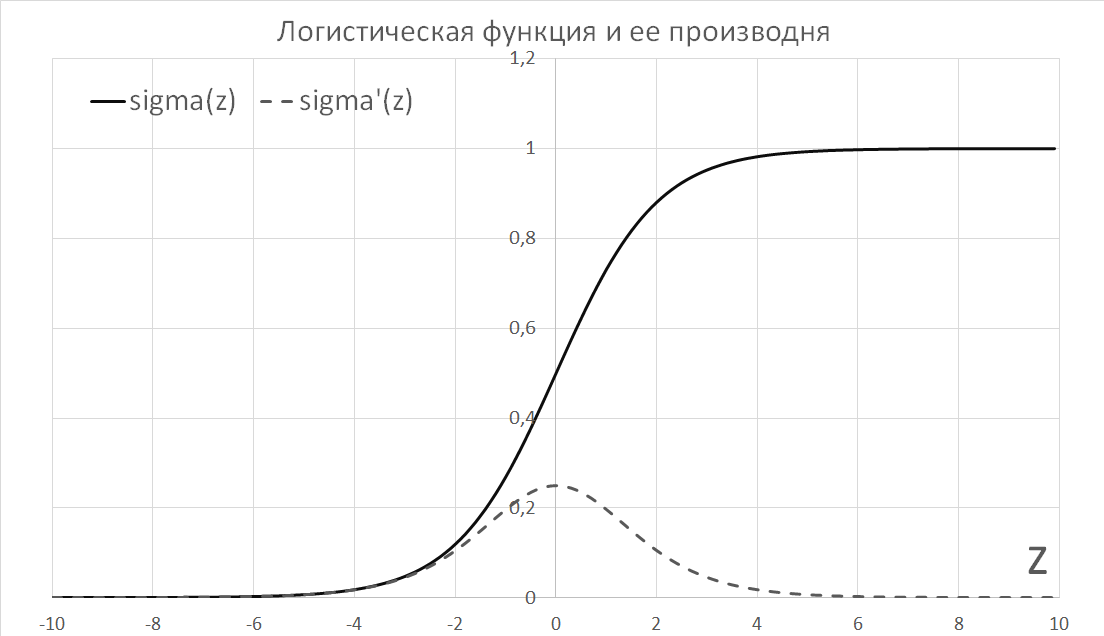
\includegraphics[width=0.65\linewidth]{./figuresch1/logistic_and_derivative.png}
     		\caption{график логиистической функции ($sigma(x)$) и ее производной ($sigma'(x)$)}		
     		\label{ch1:fig:logistic_and_derivative}
     	\end{center}
     \end{figure}

Вероятность проблемы вымывания градиента растает с ростом числа слоев в многослойном персептроне, если в большинстве случаев $\partial f(z)/\partial z < 1$ (эффект геометрической прогрессии). Это приводит к тому, что начальные слои персептрона перестают обучаться. Если в большинстве случаев  $\partial f(z)/\partial z > 1$ - происходит обратный вымыванию случай - \textbf{взрыв градиента (gradient explosion).} Данный эффект ведет к слишком большому  значению обновлений значений весов нейронной сети, это также приводит к быстрому переходу значений функций активации в область насыщения. Таким образом, в идеале $\partial f(z)/\partial z = 1$ всегда. Однако, соблюдение данного условия достаточно сложно гарантировать, особенно при увеличении числа слоев в нейронной сети. Позже в книге будут показаны, меры, позволяющие снизить вероятность вымывания и взрыва градиента. Отметим, что в настоящее время предложены нейронные сети, имеющие до 1001 слоя - при обучении которых не возникает (обходят) соответствующие проблемы.

В окончании данного раздела следует отметить, что в настоящее время в компьютерном зрении полносвязные нейронные сети (многослойный персептрон) в своей оригинальной реализации как таковые не используются. Однако, они используются в качестве \textbf{завершающих слоев (head layers)}, например, в задачах классификации, а также многих других.  При этом, в последнее время развивается альтернативный сверточномым сетям подход к компьютерному зрению, основанный на т.н. архитектурах - \textbf{трансформерах (vision transformer)}. Данный тип архитектур часто включает только полносвязные слои. \textcolor{brown}{Обзор архитектур данного типа будет дан в конце книги.}

В начале 1990-х интерес к нейронным сетям упал в силу успехов развития классических методов машинного обучения и выявленных на тот момент технических ограничений в использовании нейронных сетей. В частности, одним из наиболее перспективных на тот момент стал метод опорных векторов (support vector machine, SVM) и его ядерная модификация - kernel SVM Отметим, что метод метод опорных векторов и его ядерная модификация разработаны Вапником (уже упоминавшимся в книге)
\textcolor{red}{[??]}.
Данный метод в настоящее время может быть классифицирован как частный случай многослойного персептрона с одним скрытым слоем радиально-базисной функцией активации и особым методом обучения на основе градиентного спуска. Метод имеет сравнительно низкую вычислительную сложность и часто позволяет получить неплохую точность. Однако, современные глубокие нейронные сети обходят данный метод по точности и обобщающей способности в большинстве задач, в том числе в задачах компьютерного зрения. 

Техническими ограничениями связанными с использованием нейронных сетей на начало 1990-х являлись: проблема вымывания градиента, требования к обучению на достаточно большой выборке данных (а также поиск таких выборок и их хранение данных и) и сравнительно высокое время работы многослойных персептронов и необходимость хранить достаточно большой массив параметров (весовых коэффициентов) для их работы \cite{kelleher2019deep}. 
В настоящее время данные проблемы в той или иной степени решены, что и обуславливает популярность нейронных сетей сегодня. 

\newpage
\subsection{Идеи сверточных нейронных сетей в 1980е - 1990е}
\subsubsection{Неокогнитрон и предпосылки к сверточным сетям} 
%%%%%%%%%%%%% NEOCOGNITRON %%%%%%%%%%%%%%%%%%%%%
В 1975 г К. Фукушимой была предложена архитектура оригинальной искусственной нейронной сети - когнитрон \cite{fukushima1975cognitron}. Данная архитектура базировалась на работах по изучению принципов функционирования глаза, Одной из наиболее известных работ по этой теме является работа D. Hubbel \cite{hubel1968receptive}. Также стоит отметить, что в работах D. Hubel 1959 \cite{hubel1959receptive} и L.G.Roberts \cite{roberts1963machine} была впервые предложена идея создания систем искусственного зрения как таковых.

Когнитрон стал прообразом использования искусственных нейронных сетей в задачах компьютерного зрения. Когнитрон представлял собой многослойную сеть, каждый слой которой состоял из т.н. ускоряющих и замедляющих нейронов (excitatory, inhibitory). Каждый возбуждающий нейрон следующего слоя был связан с близлежащими нейронами предыдущего слоя. А каждый замедляющий нейрон имел входы с близлежащих нейронов своего слоя и выходные связи с возбуждающими нейронами следующего слоя. Вход каждого возбуждающего нейрона определялся отношением суммы воздействий возбуждающих к тормозящим нейронам предыдущего слоя. Иллюстрация связей двух слоев когнитрона приведена на рисунке \ref{ch1:fig:cognitron}.

%https://intuit.ru/studies/courses/88/88/lecture/20551?page=4
    \begin{figure} [!h]
    	\begin{center}
    		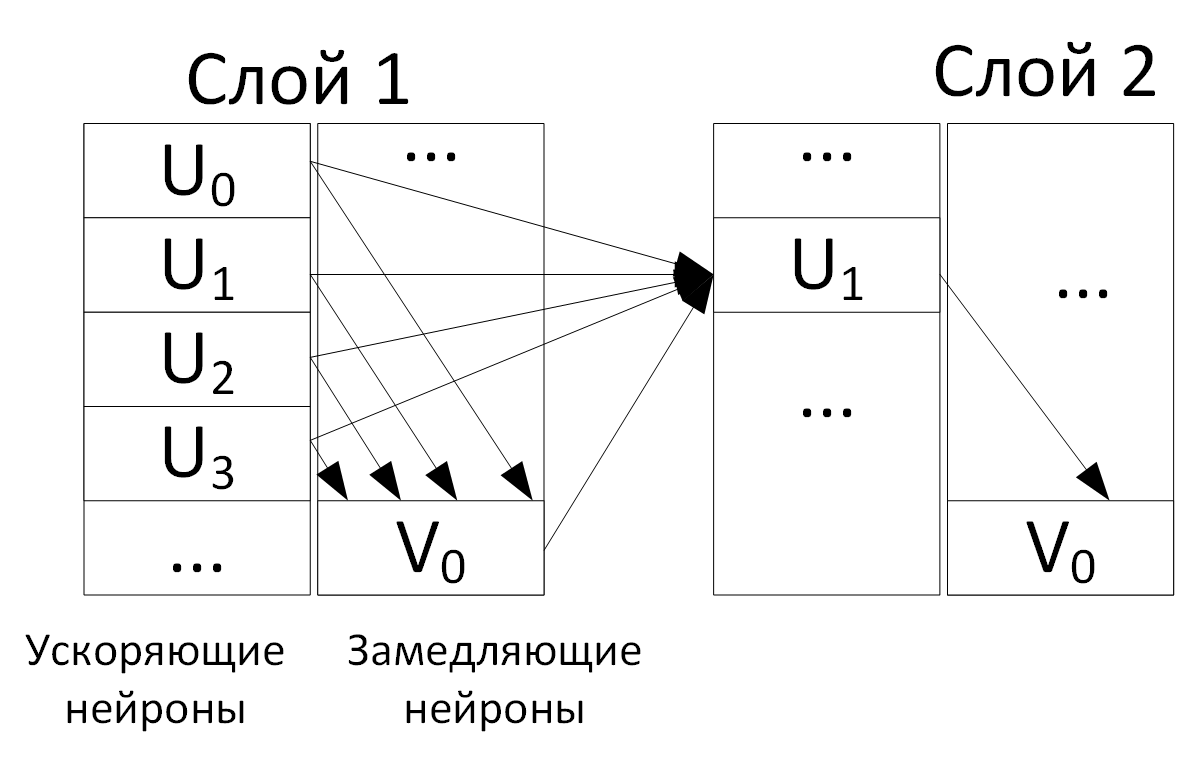
\includegraphics[width=0.5\linewidth]{./figuresch1/cognitron.png}
    		\caption{иллюстрации работы двух слоев когнитрона.}		
    		\label{ch1:fig:cognitron}
    	\end{center}
    \end{figure}
%TODO: ссылки, метрики, или это все удалить, взял от сюда: https://intuit.ru/studies/courses/88/88/lecture/20551

Отметим, что согласно оригинальной идеи когнитрон имел 2 слоя. Обучение проходило по принципу самоорганизации - таким образом, что выход второго слоя должен был описывать входное изображение. 

В 1980 году  и C. Мийяке (Fukushimo, Miyake) была предложена модифицированная архитектура нейронной сети - неокогнитрон \cite{fukushima1982neocognitron}. 
Основными отличиями новой архитектуры от когнитрона, описанной выше были:
\begin{itemize}\itemsep 0em
    \item использование многослойной архитектуры;
    \item организация нейронов каждом слое в виде двух-мерных структур;
    \item использование в каждом скрытом слое нескольких т.н. планов;
    \item использование в каждом слое простых (С-клетка) и сложных (S-клетка) нейроннов;
    \item С-клетки выполняют функции клеток возбуждения в когнетроне;
    \item S-клетки выполняют функцию выделения максимальной информации (остальная информация локальной области обнуляется) - то есть выполняют функцию нелинейности (функцию активации);
    \item снижение размеров планов с увеличением глубины слоя таким образом, что последний слой представлял собой одно число на каждый план.
\end{itemize}
Использование нескольких планов в каждом слое нейронной сети позволяет по разному выучивать сетью одни и те же признаки во входных данных (особенности входного изображения). Использование S-клеток позволяет гарантировать что выделение максимальной информации о каждом признаке в независимости от его расположения. Таким образом целью C клеток является увеличение воздействия на каждый следующий нейрон, а целью S клеток является снижение такого воздействия при минимизации выходной информации нейрона. Архитектура С и S клеток в неокогнитроне называется латентным торможением 
\cite{aksenov2006neocognitron}. Иллюстрация архитектуры неокогнитрона приведена на рисунке \ref{ch1:fig:neocognitron}. 
Понятие "план" в архитектуре неокогнитрона близки по понятию \textbf{канал или карта признаков} в современных сверточных нейронных сетях. Понятие С-клетки близко к понятию \textbf{свертка}, а понятие S-клетки близко к понятию \textbf{субдесктретизация (pooling)} в современных сверточных нейронных сетях. Кроме того использование S-клетки в качестве функций активации близко к понятию т.н. maxout функций активации. Частным случаем maxout является наиболее популярная в настоящее время функция активации ReLU (полулинейная функция активации).

    \begin{figure} [!h]
    	\begin{center}
    		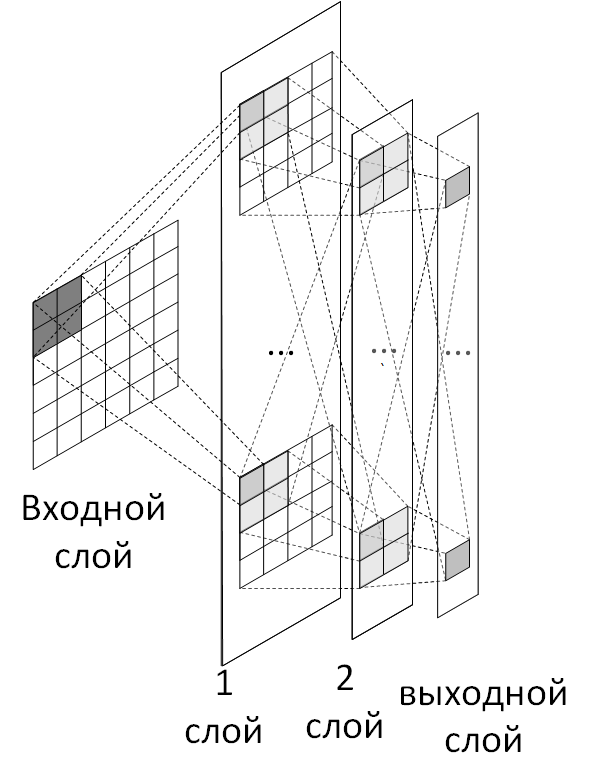
\includegraphics[width=0.45\linewidth]{./figuresch1/neocognitron.png}
    		\caption{иллюстрации архитектуры неокогнитрона. Разделение слоя на С- и S- клетки опущено.}		
    		\label{ch1:fig:neocognitron}
    	\end{center}
    \end{figure}

В основе представления данных в архитектурах когнитрон и неокогнитрон, по существу, был положены: 
\begin{itemize}
    \item принцип образования локальных связей;
    \item принцип конкуренции локальных связей;
    \item принцип образования \textbf{рецептивного поля.}
\end{itemize}
Описанные принципы заложены в основе современных глубоких сверточных нейронных сетей.
Иллюстрации локальной связанности, конкуренции локальных связей и образования рецептивного поля приведены на рисунках \ref{ch1:fig:Receptive_field_cognitron} А), Б) и В) соответственно. 

    \begin{figure} [!h]
    	\begin{center}
    		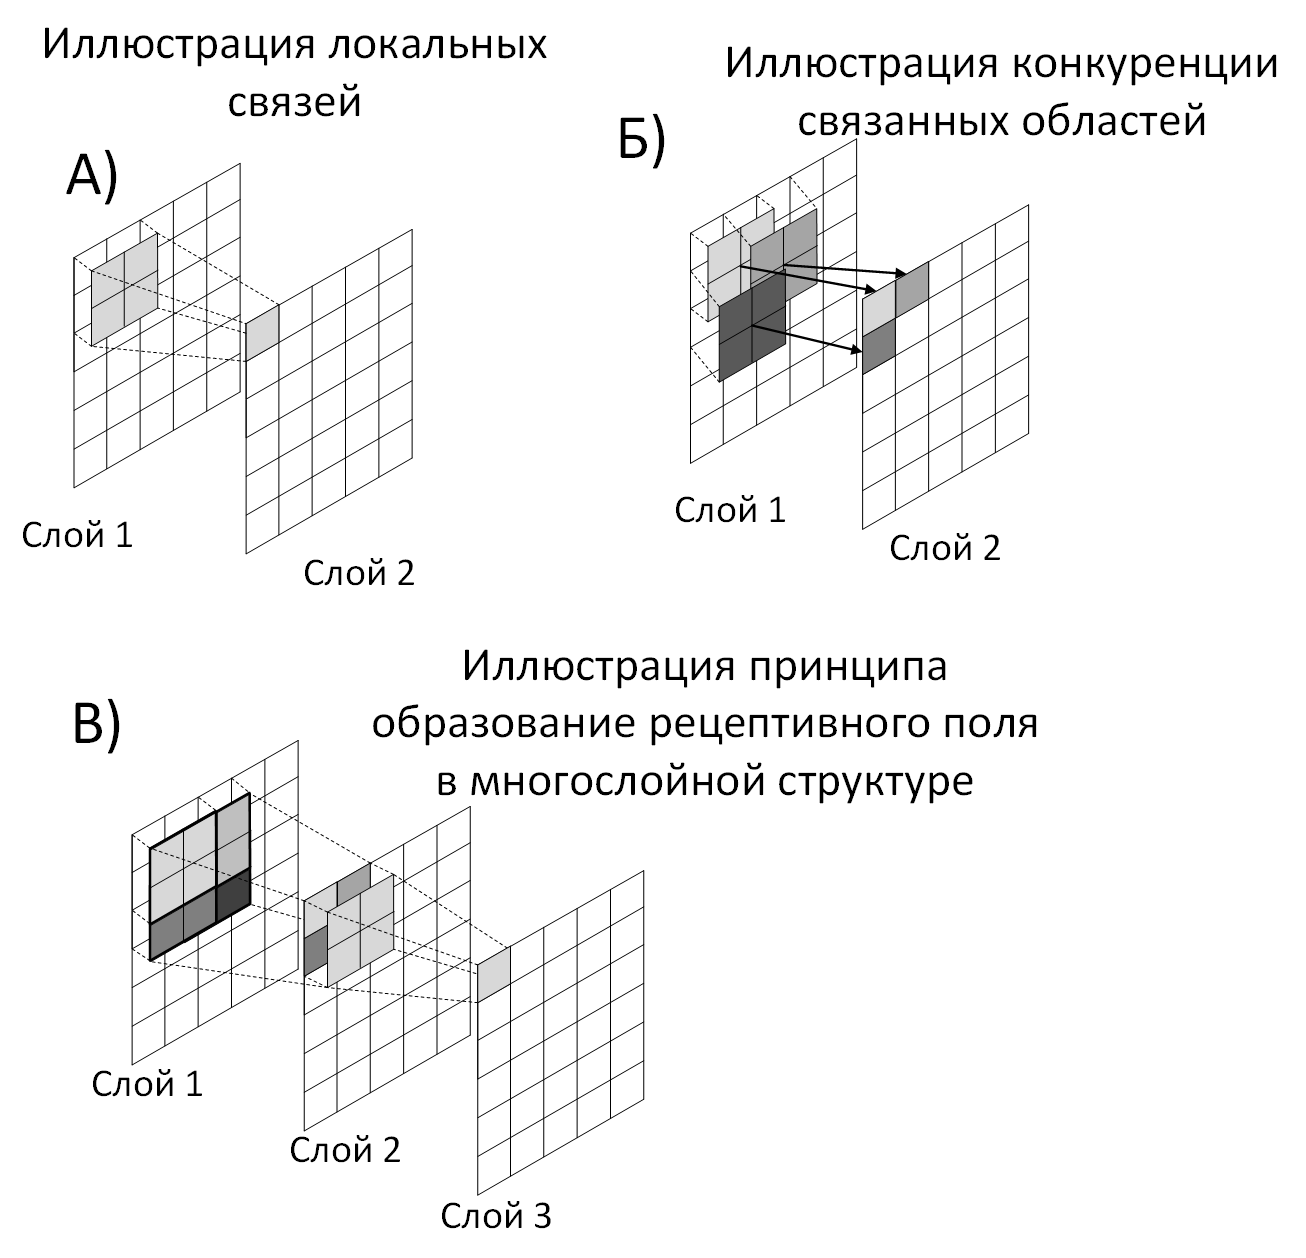
\includegraphics[width=0.9\linewidth]{./figuresch1/Receptive_field_cognitron.png}
    		\caption{иллюстрации локальной области связанности когнитрона (А), конкуренции областей связанности (Б) и образования рецептивного поля (В).}		
    		\label{ch1:fig:Receptive_field_cognitron}
    	\end{center}
    \end{figure}

\textbf{Локальная связанность} состоит в том, что каждый нейрон следующего слоя имеет связи только с близлежащими нейронами предыдущих слоев. Таким образом, каждый нейрон отвечает за информацию содержащуюся в определенной пространственно-локализованной области входного изображения (упорядоченного двух-мерного массива данных) (рис. \ref{ch1:fig:Receptive_field_cognitron} (А)). 
\textbf{Конкуренция локальных связей} заключается в том, что каждый участок входных данных может быть по разному учтен в разных нейронах следующего слоя (с разным весовым коэффициентом) (рис. \ref{ch1:fig:Receptive_field_cognitron} (Б)). Принцип локальной связанности позволяет сжать информацию с предыдущих слоев взвешенным суммированием. Конкуренция локальных связей позволяет избежать потери важной информации с предыдущего слоя за счет ее дублирования в разных нейронах. 

\textbf{Принцип образования рецептивного поля} состоит в том, что в многослойной структуре нейроны каждого следующего слоя включают информацию сразу об локальной области нейронов предыдущего слоя. Таким образом, с увеличением количества слоев, каждый нейрон последующего слоя содержит в себе информацию о все большей области входного изображения (рис. \ref{ch1:fig:Receptive_field_cognitron} (В)). 
В силу локальности связей нейроны начальных слоев содержат в себе сравнительно простые составные части входного изображения, называемые \textbf{низкоуровневые признаки}. 
Каждый низкоуровневый признак сам по себе несет сравнительно мало информации - то есть "почти наверное" не позволяет сделать однозначный вывод о содержании входных данных. Однако, с увеличением числа слоев в нейронной сети возрастает и сложность признаков - каждый признак несет в себе все больше информации о входных данных - то есть повышается вероятность однозначного сопоставления входных данных целевому результату. 
Описанные признаки называются \textbf{высокоуровневые признаки}.
Иллюстрация возможности выделения низкоуровневых  и высокоуровневых признаков при помощи рецептивного поля многослойной нейронной сети c локальной связанностью приведена на рисунке 
\ref{ch1:fig:receptive_field_feature_level}. Отметим, что принцип рецептивного поля был предложен в 1962 г в работе D. Hubel \cite{hubel1962receptive} в ходе анализа зрительной системы животных. Также следует отметить работу \cite{marr1982vision}, в которой    исследована иерархическая структуры глаза и многослойный принцип образования в нем рецептивного поля. 
    
    \begin{figure}
    	\begin{center}
    		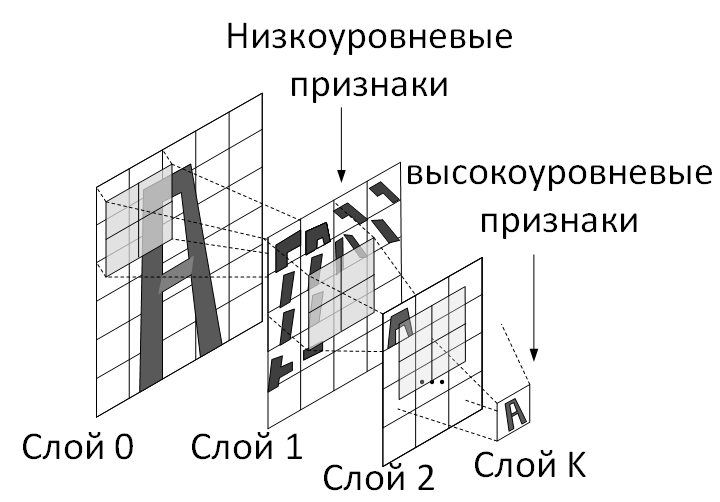
\includegraphics[width=0.7\linewidth]{./figuresch1/receptive_field_feature_level.png}
    		\caption{Иллюстрация возможности выделения низкоуровневых  и высокоуровневых признаков при помощи рецептивного поля многослойной нейронной сети с локальной связанностью.}		
    		\label{ch1:fig:receptive_field_feature_level}
    	\end{center}
    \end{figure}

В 1988 была предложена инвариантная к сдвигу искусственная нейронная сеть (SIANN, shift-invariant artificial neural network) - фактически ставшая прообразом сверточных нейронных сетей \cite{zhang1988shift}.  Сеть содержала два скрытых слоя, каждый из которых был организован подобно С-клеткам нейрокогнитрона + функция активации. В качестве функций активации использовались т.н. двойные сигмоиды ($f(z)= 2/(1+\exp(-z))-1$). Сеть обучалась методом обратного распространения ошибки. Варианты модификаций данной архитектуры активно изучались в 1990-х \cite{hasegawa1998shift}. Однако сегодня данная архитектура может быть рассмотрена только как подкласс сверточных нейронных сетей \cite{li2021survey}. Также в 1989 году была описана архитектура одномерной сверточной нейронной сети для решения задач распознавания звуковых фонем \cite{waibel1989phoneme}.

\subsubsection{Архитектура ConvNet} 
%%%%%%%%%%%%%%%%% CONVNET 1989 %%%%%%%%%%%%%%%%%%%%%%%%%%
В 1989 г. Яном Лекуном была предложена первая сверточная нейронная сеть ConvNet \cite{lecun1989backpropagation}. Нейронная сеть была  для решения задачи распознавания рукописных цифр по их фотографиям \cite{lecun1989generalization}. 
\uline{Архитектура ConvNet была первой сверточной нейронной сетью (convolutional neural network ,CNN) в современном понимании данного типа архитектур 
}. 
В частности, в работе \cite{lecun1989generalization} термин сверточные нейронные сети (convolutional neural networ, CNN) был впервые популяризован \cite{li2021survey}.
Нейронная сеть ConvNet была успешно применена для распознавания рукописных цифр на почтовых индексах \cite{lecun1989backpropagation}. 
Иллюстрация архитектуры ConvNet, описанная в работе \cite{lecun1989backpropagation} приведена на рисунке \ref{ch1:fig:convnet1989}. 

\begin{figure}[!h]
	\begin{center}
		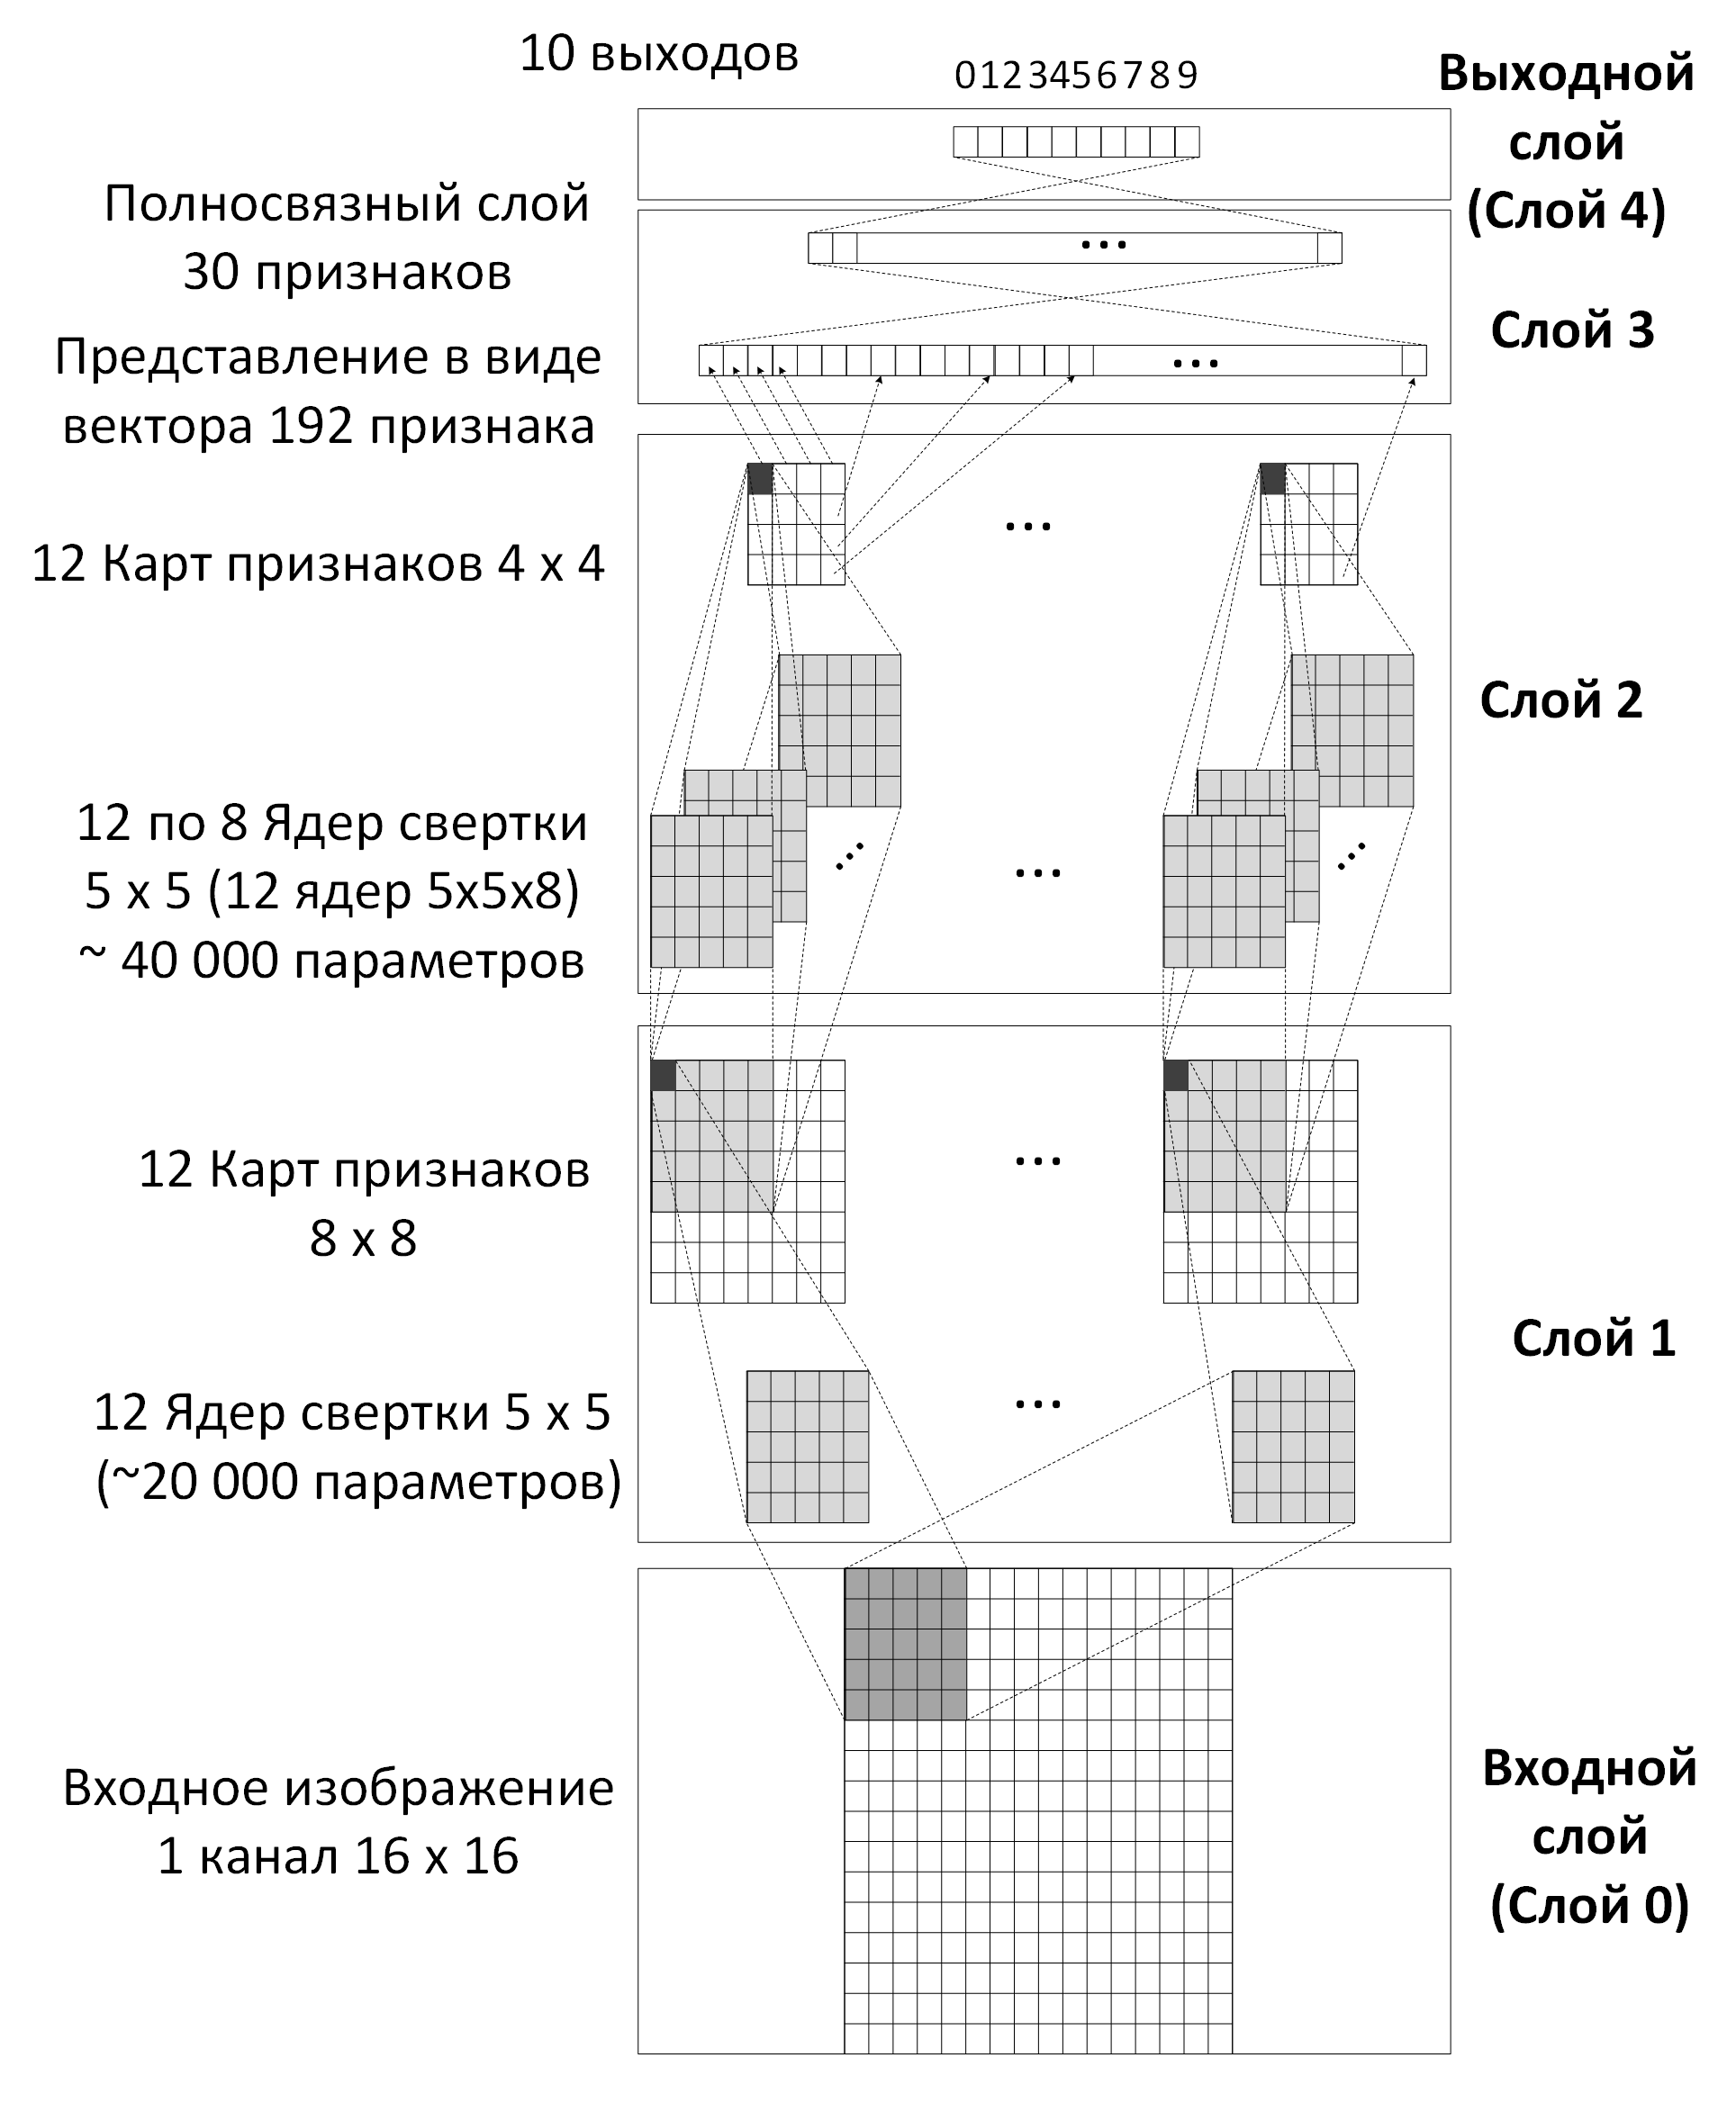
\includegraphics[width=0.99\linewidth]{./figuresch1/convnet1989_v2.png}
		\caption{Иллюстрация архитектуры сверточной нейронной сети ConvNet 1989 г.}		
		\label{ch1:fig:convnet1989}
	\end{center}
\end{figure}
Архитектура ConvNet обучалась методом обратного распространения ошибки, в качестве функции потерь использовался средний квадрат ошибки. В качестве функций активации - логистические функции. Нейронная сеть имела 3 скрытых слоя, два их которых сверточные и один полносвязный. Выходной слой также полносвязный и имеет 10 выходов по одному для каждой цифры. 
В основе архитектуры ConvNet (рис. \ref{ch1:fig:convnet1989}) лежит понятие двухмерной свертки. Данное понятие является основополагающим для сверточных нейронных сетей. Основная идея использования свертки в нейронных сетях заключается в замене полносвязного слоя на одно или несколько сравнительно небольших сверточных ядер (не больших по общему числу параметров). 

В случае одного двух-мерного ядра и одного канала изображения запишем операцию свертки в следующем виде:
\begin{equation}
    r[i,j] = (k\ast x)[ij] = \sum_{a=0}^{h_k-1}\sum_{b=0}^{w_k-1}k[a,b]x[i+a,j+b], 
\end{equation}
где:
\begin{itemize}
\itemsep 0em 
    \item $k[a,b]$ - значение ядра свертки с координатами $[a,b]$ ($k$ имеет размерность $h_k \times w_k)$;
    \item $x[i,j]$ - значение входного двухмерного массива с координатами $[i,j]$ ($x$ имеет размерность $h_x \times w_x$);
    \item $r[i,j]$ - значение результата свертки с координатами  $[i,j]$ ($r$ имеет размерность $h_x-h_k+1 \times w_x - w_k +1$);
    \item $\ast$ - операция свертки.
\end{itemize}

% Иллюстрация двухмерной свертки приведена на рисунках \ref{ch1:fig:2d_conv_stride_1_v2} и \ref{ch1:fig:2d_conv_stride_1} в двух разных формах. 
% \begin{figure}[!h]
% 	\begin{center}
% 		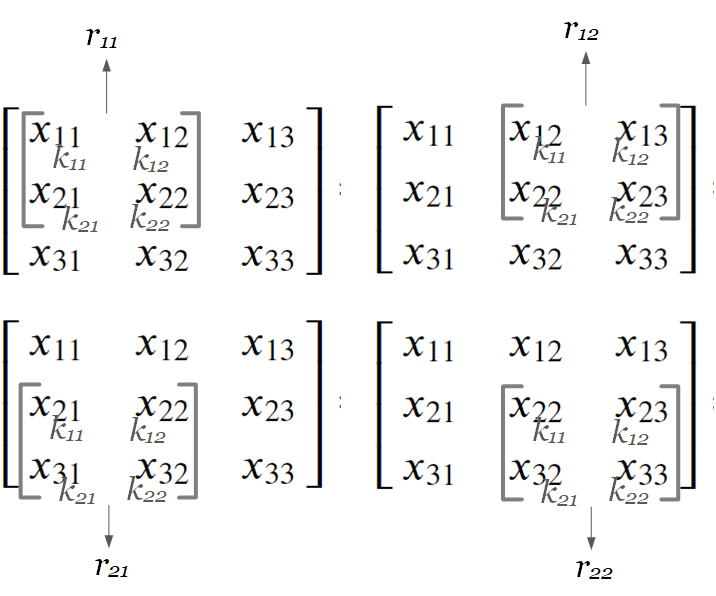
\includegraphics[width=0.7\linewidth]{./figuresch1/2d_conv_stride_1_v2.png}
% 		\caption{Иллюстрация двухмерной свертки $2 \times 2$}		
% 		\label{ch1:fig:2d_conv_stride_1_v2}
% % 	\end{center}
% % \end{figure}

% % \begin{figure}
% % 	\begin{center}
% 		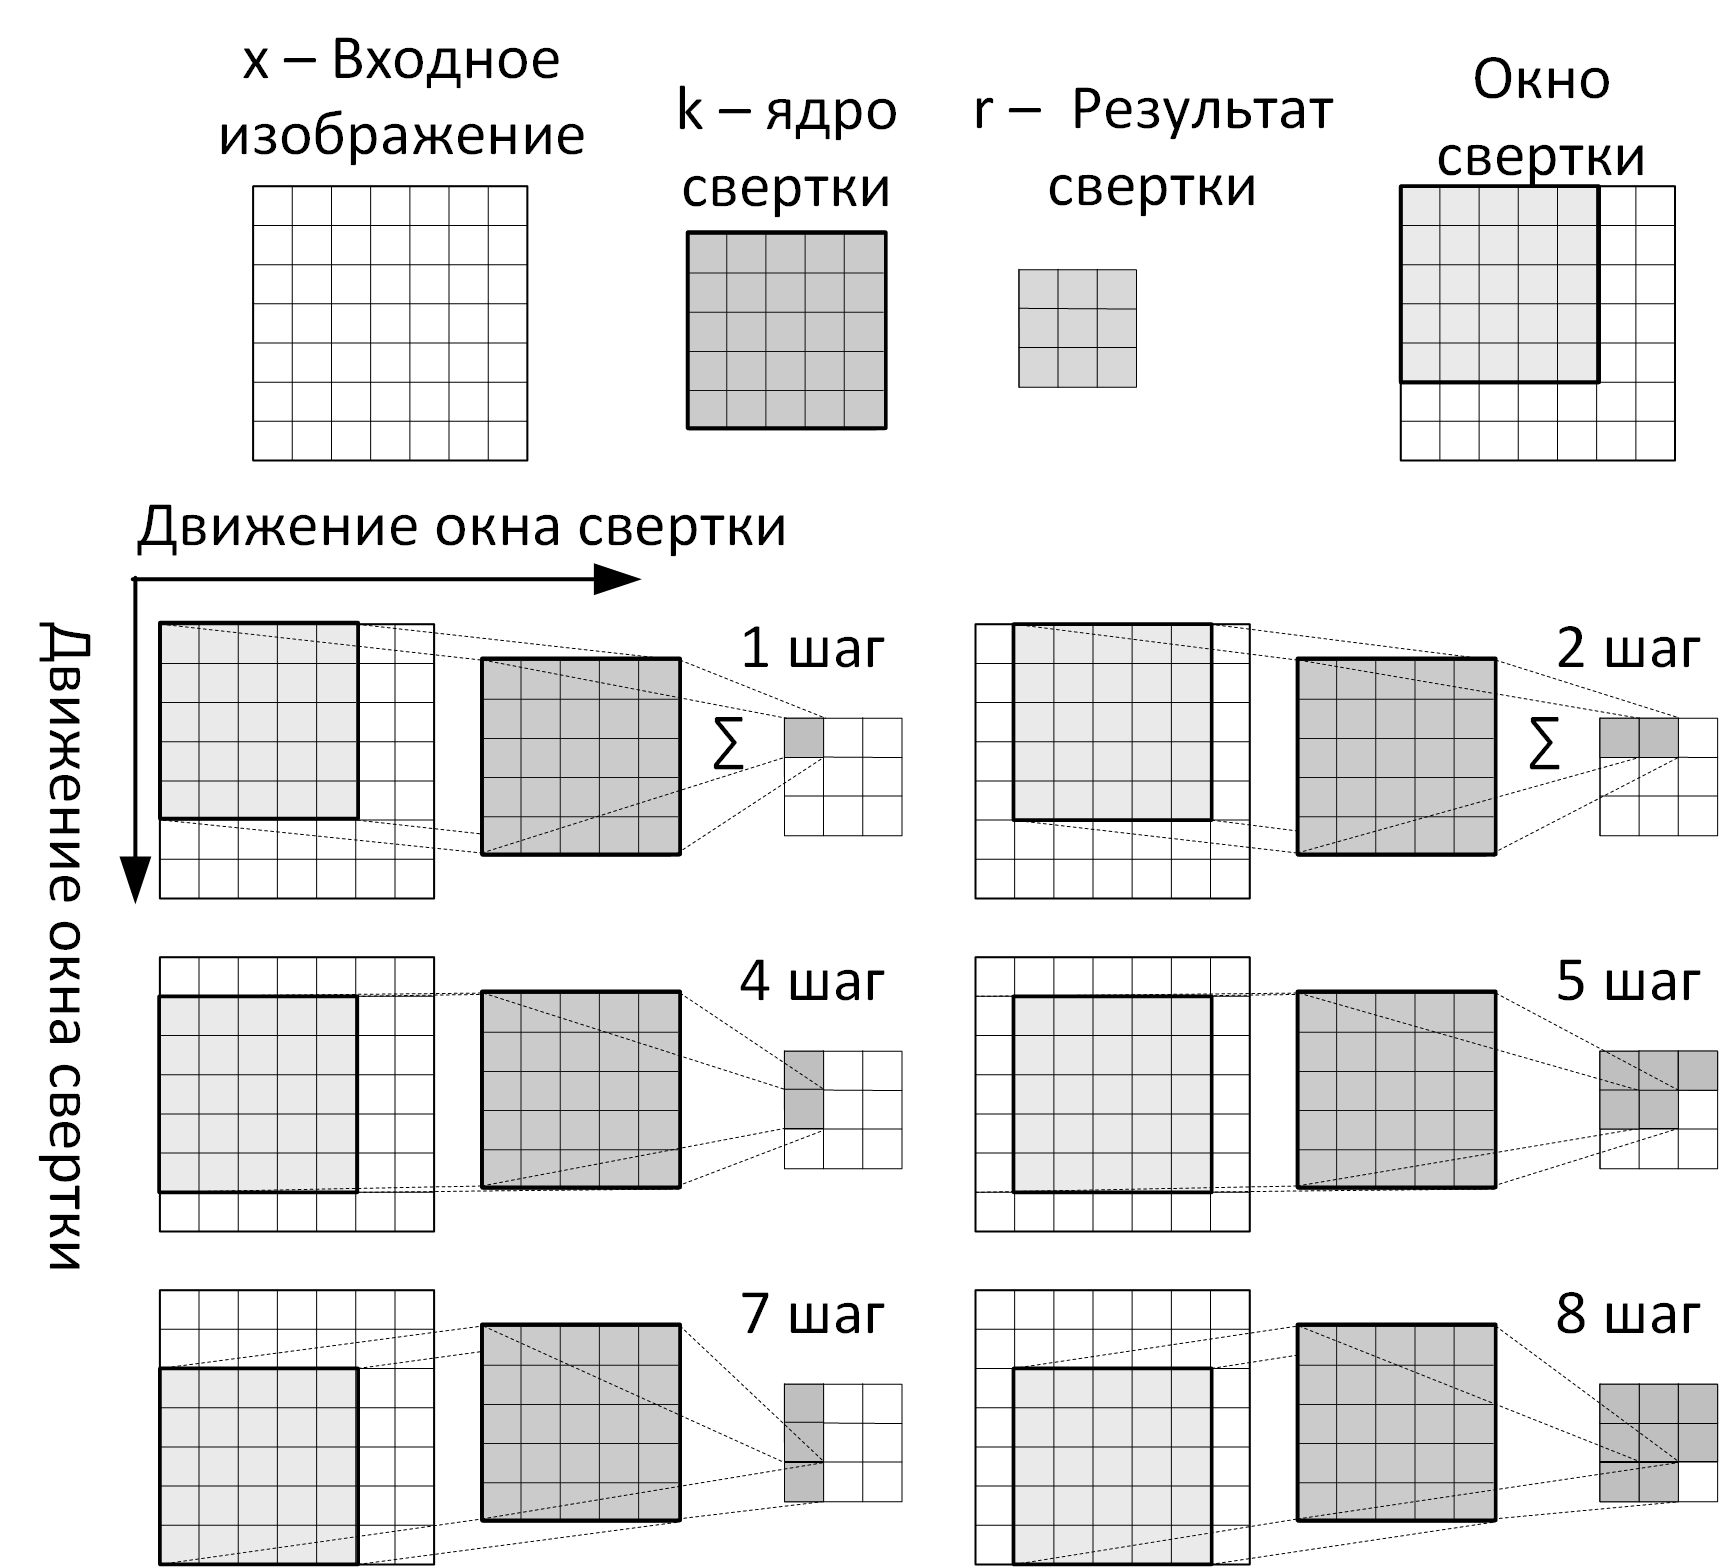
\includegraphics[width=0.76\linewidth]{./figuresch1/2d_conv_stride_1_v3.png}
% 		\caption{Иллюстрация двухмерной свертки $5 \times 5$}		
% 		\label{ch1:fig:2d_conv_stride_1}
% 	\end{center}
% \end{figure}

%TODO: возможно надо переписать
Каждый сверточный слой нейронной сети ConvNet (рис. \ref{ch1:fig:convnet1989}) образован несколькими наборами двухмерных сверток. 
Каждое двухмерное ядро свертки имеет свои значения весовых параметров.
\uline{
Результатом воздействия каждого сверточного ядра является карта признаков. Каждая карта выделяет свои признаки (но признаки одно уровня для одного слоя)}.  

\uline{Каждый набор ядер свертки может быть описан многомерной структурой, которая в широком смысле может быть названа \textbf{тензор}}. Например, слой 1 (рис. \ref{ch1:fig:convnet1989}) можно описать при помощи трехмерных тензоров сверточных ядер и карт признаков на выходе слоя. В случае слоя 2 (рис. \ref{ch1:fig:convnet1989}) имеется набор  трехмерных тензоров сверточных ядер (четырех мерный тензор) и трехмерная карат признаков на выходе. При этом каждый элемент каждой карты образован суммой результатов соответствующих ей двухмерных сверточных ядер со смещением ( \textbf{параметр смещения -bias} - дополнительный параметр каждого ядра). 

%TODO: возможно это следует убрать
Таким образом для выхода слоя 2:
\begin{equation}
    \label{ch1:eqn:conv_3d_4d}
    r[c_{out}, i,j] = (k\ast x)[c_{out},i,j] = \sum_{c=0}^{C-1}\sum_{a=0}^{h_k-1}\sum_{b=0}^{w_k-1}k[c_{out}, c, a,b]x[c,i+a,j+b] + \theta[c_{out}],
\end{equation}
где 
\begin{itemize}
\itemsep 0em 
    \item $C$ - число каналов свертки для входного массива; 
    \item $x[c, i,j]$ - значение канала $c$ входного массива с координатами $[i,j]$ ($x$ имеет размерность $C\times h_x \times w_x$);
    \item $c_{out} = 0,...,C_{out}-1$ - число выходных карт признаков;
    \item $\theta[c_{out}]$ - смещение результата свертки ядра $k[c_{out},:,:,:]$ (каждого ядра);
    \item $r[c_{out}, i,j]$ - значение выходной карты признаков $c_{out}$;
    \item $k[c_{out}, c, a,b]$ - 4-х мерный массив ядер свертки;
    \item $\theta[c_{out}]$ - смещение ядра свертки.
\end{itemize}
%TODO: убрать до сюда!

%%%%%%%%%%%%%%%%%%%%%% SOFT MAX
\subsubsection{Функция активации softmax}

В 1989-1990 годах в работах \cite{bridle1990training, bridle1990probabilistic} было предложено использование в выходном слое нейронных сетей функцию активации softmax вместо набора выходов, каждый из которых имел свою логистическую функцию активации. Так, например, в работе \cite{lecun1989generalization}  архитектура ConvNet1989 использовалась для решениях задача распознавания рукописных цифр. При этом сеть имела 10 выходных нейронов - каждый для одной цифры от 0 до 9 (см. рис. \ref{ch1:fig:convnet1989}). Каждый нейронов имел свою логистическую функцию (\ref{ch1:eqn:sigmoid}). Результатом работы сети выбирался ответ с максимальным значением (\textbf{принцип победитель получает все}). Однако, такой подход затрудняет интерпретацию результатов, особенно если результатов будет не 10, а скажем 100. \textit{Например, пусть для одной эпохи обучения мы получили для двух выходов сети значения 0,95 и 0,92, а для следующей эпохи 0,96 и 0,955 - как понять на какой эпохе обучение было оптимальным?} Функция softmax позволяет устранить описанную проблему. В случае с функцией softmax результаты всех выходов нейронной сети нормируются так, чтобы в сумме всегда была 1. Тогда каждый результат можно интерпретировать как вероятность того, что, один экземпляр входного набора данных соответствует одному значению выходных данных (например, одному номеру метки класса). Функция $\mathrm{softmax}$ и ее производная $\mathrm{softmax}'$ может быть записана следующим образом:
    \begin{equation}
    \label{ch1:eqn:softmax}
        \mathrm{softmax}(z_i) = \dfrac{\exp(z_i)}{\sum_{c=0}^{C-1}\exp(z_c)}, \ \ \  \mathrm{softmax}'(z_i) = \mathrm{softmax}(z_i)(1-\mathrm{softmax}(z_i))
    \end{equation}
где $C$ - число классов; $z_i$ - входное значение функции - т.н. \textbf{логит (logit)}, (например для многоклассовой логистической регрессии $z_i = \sum_{j=0}^{N-1}w_{ij}x_j$, где $w_{ij}$ матрица весов размером $C\times N$,  $x_j$ - набор входных значений).

Для реализации функции softmax нейронная сеть должна иметь $C$ выходных нейронов без функций активации для каждого.Вектор результирующих значений выходных нейронов должен быть пересчитан для каждого значения по формуле  \ref{ch1:eqn:softmax}. Результатом работы нейронной сети считается номер позиции максимального значения вектора:
    \begin{equation}
    \label{ch1:eqn:softmax_result}
        \hat y = \mathrm{arg\max_i}(\mathrm{softmax}(z_i)),
    \end{equation}
где $\mathrm{arg\max_i}$ - функция номера позиции с максимальным значением; $\hat y$ - результат работы алгоритма. 
Иллюстрация работы слоя, реализующего выражения (\ref{ch1:eqn:softmax}) и (\ref{ch1:eqn:softmax_result}) приведена на рисунке
\begin{figure}[!h]
	\begin{center}
		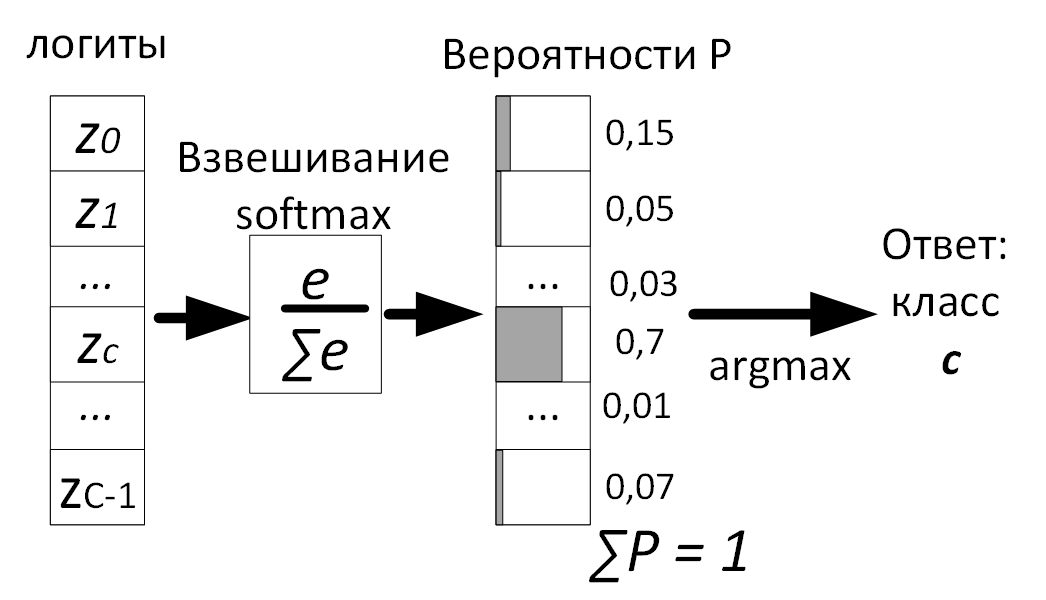
\includegraphics[width=0.75\linewidth]{./figuresch1/softmax.png}
		\caption{Иллюстрация работы выходного слоя нейронной сети с функцией активации softmax}		
		\label{ch1:fig:softmax}
	\end{center}
\end{figure}

При обучении нейронной сети с функцией активации выходного слоя softmax схема работы будет несколько отличаться от проиллюстрированной на рис. \ref{ch1:fig:softmax}. Так как во время обучения номер целевого класса известен вместо выражения \ref{ch1:eqn:softmax_result} вероятность класса будет оцениваться и максимизироваться именно для целевых классов. 

В работе \cite{lawrence1997face} 1997 года преимущества использования функции softmax были показаны для задачи распознавания лиц по фотографиям с использованием сверточной нейронной сети и ряда других алгоритмов. 
% Отметим, что для случая бинарной классификации (да/нет) функция softmax тождественна логистчиеской функции. 

Отметим, что в современных нейронных сетях задачи классификации можно разделить на три вида:
\begin{itemize}
    \item \textbf{задачи бинарной классификации} - необходимо оценить только наличие или отсутствие одного класса (например, есть или нет кошка на изображении); один выходной нейрон, выходная функция активации - логистическая функция;
    \item \textbf{задачи много-классовой классификации} - необходимо оценить наличие одного из нескольких классов (например, оценить это слон, собака или кошка); $С$ выходных нейронов, выходная функция активации softmax;
    \item textbf{задачи много-меточной классификации}-  необходимо оценить вероятность наличия по каждому  классу одновременно (например одновременно оценить есть ли на изображении и кошки и собаки и слоны) - $С$ выходных нейронов,, для каждого выходная функция активации - логистическая функция.
\end{itemize}    
Также следует отметить, что \textbf{если решается задача регрессии} (например определить позицию или длину кошки), то используется число нейронов, равное числу оцениваемых параметров, каждый выходной нейрон не имеет функции активации. 

\subsubsection{Архитектура LeNet 5} 
%%%%%%%%%%%%%%%%%%%%%%%%%%%%%%% LENET 1998
\uline{В 1998 Яном Лекуном была предложена модифицированная относительно  ConvNet (рис. \ref{ch1:fig:convnet1989}) нейронная сеть \textbf{LeNet5} \cite{lecun1998gradient}}. Данная нейронная сеть была применена для распознавания рукописных цифр без предварительной обработки изображений. 
Также в работе \cite{lecun1998gradient} был впервые использован набор данных  - рукописных MNIST (Modifyed NIST), который в настоящее время является одним из наиболее популярных в задачах компьютерного зрения (набор доступен по ссылке \cite{MNISTlecuncom}.
Иллюстрация архитектуры нейронной сети LeNet5 приведена на рисунке \ref{ch1:fig:LeNet5}. По существу, большинство современных сверточных нейронных сетей (на момент написания книги) являются наследниками архитектуры LeNet5. Более того LeNet5 часто является базовой архитектурой, с которой проводятся сравнения более совершенных архитектур. Также архитектура LeNet стала первой, доказавшей, что системы распознавания, основанные на автоматическом обучение (нейронные сети) могут работать лучше чем системы, основанные на вручную описанных эврестических правилах (классические методы машинного обучения) 
\cite{lecun1998gradient}. 
Отметим, что помимо архитектуры LeNet5 в работе \cite{lecun1998gradient} были рассмотрены и другие варианты систем компьютерного зрения, не показавшие высокой точности в рассмотренной задаче. В частности графовые нейронные сети, сети пространственного смещения, классификаторы не основе метода ближайших соседей и метод опорных векторов, а также некоторые другие.

\begin{figure}[h]
	\begin{center}
		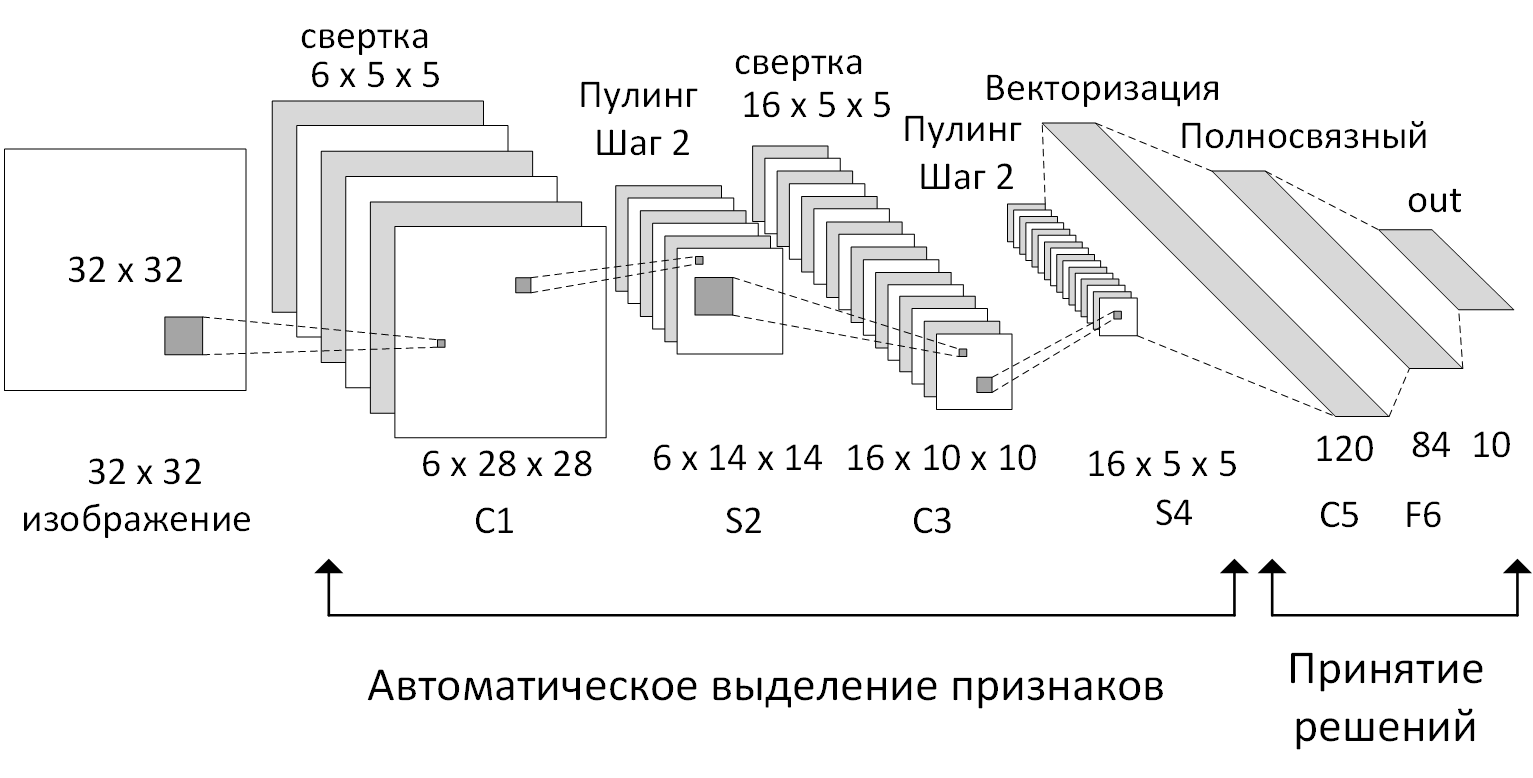
\includegraphics[width=0.99\linewidth]{./figuresch1/LeNet5_v2.png}
		\caption{Иллюстрация архитектуры сверточной нейронной сети LeNet5}		
		\label{ch1:fig:LeNet5}
	\end{center}
\end{figure}

Архитектура СНС LeNet5 включает в себя 5 слоев (2 сверточных слоя, 2 полносвязных слоя и 1 выходной слой). 
% TODO: возможно это лишнее
% \textcolor{red}{
% В качестве функций активации использовались функции масштабированного гиперболического тангенса:
% \begin{equation}[!h]
%     \label{ch1:eqn:tanh}
%     f(x) = Atanh(Sx),
% \end{equation}
% где $tanh(x)$ - гиперболический тангенс (насыщения -1 x<0 +1 x.0); A и S - регулируемые коэффициенты - т.н. г\textbf{иперпараметры}. 
% Последний слой использовал радиально базисные функции, которые реализованы так, что для каждого из 10 выходов $y_j = \sum_{i=0}^{83}(x_i-w_{ij})^2$. В качестве функции потерь использовался мульти-целевая бинаная энтропия + средний квадрат ошибки (multilabel). 
% $E = $
% }

В отличии от ConvNet 1989 г в архитектуре LeNet5 каждый сверточный слой дополнен операцией \textbf{субдискретизация (пулинг, pooling)} \cite{lecun1998gradient}. 
Идея слоя пулинга уже упоминалась ранее касательно неокогнитрона. Однако, в LeNet она имеет несколько иной смысл. Слой субдескретизации позволяет снизить размерность карт признаков. Предполагается, что при этом не произойдет потери информации. Для проведения субдескретизации по карте признаков устанавливается окно (например размером $2\times 2$ скользящее по карте с шагом $2$ (возможны и другие варианты). В каждом окне формируется одно значение (в LeNet5 среднее значение - \textbf{average pooling}):
\begin{equation}
    \label{ch1:eqn:av_pool}
    r\left[\frac{i}{s},\frac{j}{s}\right] = \sum_{a=i}^{i+w_p}\sum_{b=j}^{j+h_p}x[a,b],
\end{equation}
где:
\begin{itemize}
\itemsep 0em 
    \item $r\left[\dfrac{i}{s},\dfrac{j}{s}\right] $ - результат операции пулинг (размерность $w_r\times h_r$);
    \item $x[a,b]$ - входной двух-мерный массив (размерность $w_x\times h_x$);
    \item $w_p\times h_p$ - размеры окна пулинга;
    \item $s$ - шаг перемещения окна пулинга;
    \item $w_r = \dfrac{w_x - w_p}{s} + 1; h_r = \dfrac{h_x - h_p}{s} + 1$.
\end{itemize}

Иллюстрация работы пулинга приведена на рисунке \ref{ch1:fig:pooling}. Следует отметить, что использование субдискретизации потенциально может привести к потери информации. По этому \uline{каждый слой, содержащий субдескретизацию должен иметь увеличенное число карт признаков по сравнению с предыдущим слоем (как правило удвоенное)} - для компенсации возможных потерь. Автором LeNet также постулируется общее положение: \textbf{\uline{снижение пространственного разрешение в нейронной сети должно сопровождаться пропорциональным увеличением числа карт признаков}.}

\begin{figure}[h]
	\begin{center}
		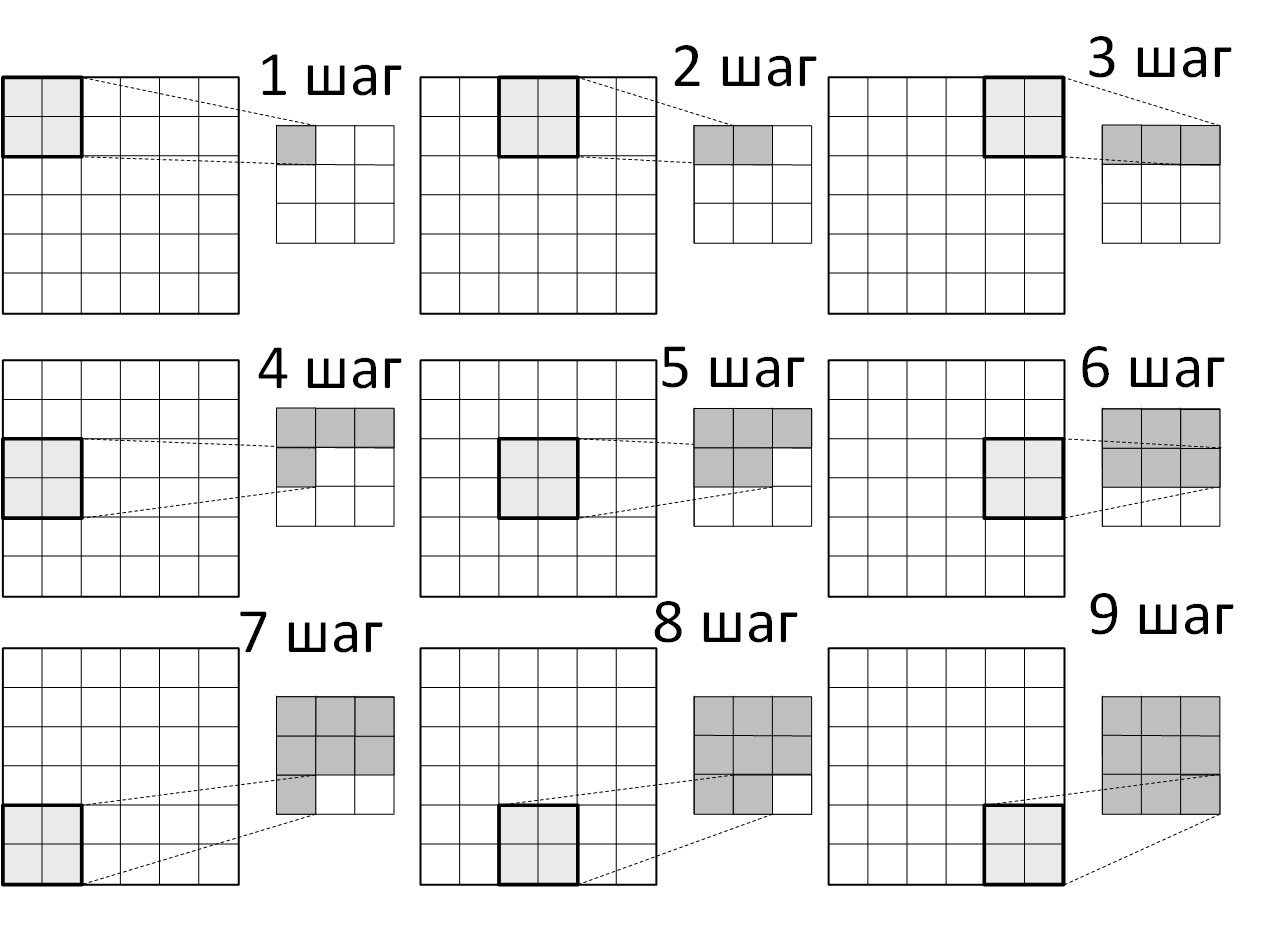
\includegraphics[width=0.7\linewidth]{./figuresch1/pooling.png}
		\caption{Иллюстрация принципа работы пулинга}		
		\label{ch1:fig:pooling}
	\end{center}
\end{figure}

Также следует отметить, что в настоящее время операция субдескретизации, в виде, описанном выше (\ref{ch1:eqn:av_pool})- локальный усредняющий пулинг используется редко. Это связано с неустойчивостью усреднения к шумам и выбросам в данных. Наиболее популярный на сегодняшний день вид субдискретизации - максимальный пулинг (\textbf{макспулинга, maxpooling}). Результатом работы макспулинга является число с наибольшей интенсивностью среди всех выделенным окном субдискретизации - то есть с наибольшей информацией.
\begin{equation}
    \label{ch1:eqn:max_pool}
    r\left[\frac{i}{s},\frac{j}{s}\right] = \max_{a,b}x[a,b], \ a=i,...,i+w_p, b=j,...,j+h_p.
\end{equation}
Идея макспулинга уже упоминалась в приложении к неокогнитрону, где она называлась S-клетка. Однако, окончательно данная идея была сформулирована в работе \cite{weng1992cresceptron} в 1992 году \cite{schmidhuber2015deep}.

По существу, нейронная сеть LeNet и все архитектуры на ее основе состоит из двух основных частей:
\begin{itemize}
    \item 1 часть: \textbf{энкодер признаков - система автоматического выделения признаков (feature extractor)} - каскад сверточных слоев.
    \item 2 часть: \textbf{головная часть - решения задачи  - в данном случае многослойный персептрон}. Данная часть архитектуры может быть выбрана различным способом в зависимости от задачи. 
\end{itemize}

В классических методах машинного обучения предполагается наличие лишь части 2 из описанных выше. При этом признаки - входные данные части 2 в классических методах выделяются вручную (например основываясь на некоторых математических моделях решаемой задачи или эвристически - на основе наблюдений). В архитектуре LeNet не требуется решение проблем подбора или выделения признаков из данных, их описания и т.д. эта задача решается в ходе обучения нейронной сети. Такой подход особенно полезен в системах компьютерного зрения - где, как уже было сказано выше, формальное описание задачи вручную крайне сложно, если вообще возможно. 

Также следует отметить, что часть 1 описанного выше разделения архитектуры НС, выделяет признаки аналогично концепции рецептивного поля, описанной выше (см. неокогнитрон). Таким образом, чем глубже сеть (чем больше слоев в энкодере признаков) тем большая область входного изображения может быть обработана. То есть чем больше слоев - тем более высокоуровневый признак и признак большего размера может быть выделен во входном изображении. 

%TODO: Надо наверно Переписать
Однако, подход  LeNet имеет ряд ограничений по сравнению с классическими методами машинного обучения. Во-первых, подход требует большего времени обучения и большего размеры выборки данных - так как помимо головной части системы необходимо обучить энкодер признаков. Во-вторых, НС требует больше ресурсов для работы (память, вычислительные ресурсы) - так как НС имеет больше параметров, чем классические системы. В-третьих, НС не могут обучаться он-лайн - в ходе своей работы. То есть можно обучить НС, использовать ее, и копить новую информацию и данные, затем, если нужно, то необходимо полностью переобучать НС и использовать уже новый результат на практике.  
Отметим, что на практике данные ограничения не снижают применимости НС в задачах компьютерного зрения и многих других. 

По задумке автора архитектура нейронной сети LeNet обладала следующими полезными свойствами инвариантности. Данные свойства полезно указать, так как они являются частью общих достоинств сверточных нейронных сетей перед другими алгоритмами обучения \cite{lecun1998gradient, lecun2015deep}.
\begin{itemize}
    \item \textbf{Инвариантность к масштабу} целевой сцены (или объекта) на входном изображении (в некоторых пределах). Инвариантность достигается за счет реализации концепции локального рецептивного поля по средствам регулирования глубины энкодера признаков и размерах ядер свертки. 
    
    \item \textbf{Инвариантность к положению} целевой сцены (или объекта) на входном изображении. Инвариантность достигается за счет пере-использования весовых параметров (использование свертки) в приманенная к разным частям изображения. 
    В частности в работе \cite{lecun1998gradient} отмечается, что если объект на входном изображении сдвинуть, то и объекты на каждой карте признаков сдвинуться, но не изменится - сам признак останется выделанным. Однако, если на изображении есть несколько сцен и их взаимные позиции изменились, то инвариантность к этой ситуации может не сохраниться \cite{lecun1998gradient}.  
    
    % надо пункт переписать.
    \item \textbf{Инвариантность к искажению} целевой сцены (или объекта) на входном изображении (в некоторых пределах) - то есть расширение обобщающей способности. Инвариантность достигается за счет использования слоев субдискретизации. Таким образом, из каждой области каждой карты признаков будет выделена лишь наиболее информативная составляющая. При этом предполагается, что небольшие искажения тестовых объектов по отношению к тренировочным не дадут высокой интенсивности - так как под них НС не обучена. Другими словами ядра свертки не коррелируют с искажениями на которых они не обучены и дадут что то около нуля.
    
    \item Переиспользование весовых параметров (использование свертки, \textbf{пространственная инвариантность весовых параметров}). При этом при использовании сверток, в отличии от нейронов неокогнитрона, в СНС число параметров меньше чем в полносвязных НС. Так для LeNet5 число тренируемых параметров $\sim 60 000$, а аналогичная полносвязная НС имела бы $\sim 340 000 параметров$.
\end{itemize}

\textit{Отметим также деталь архитектуры LeNet5, полезную с точки зрения дальнейшего изложения материала:
В слои 3 фактически \textbf{использовалась групповая свертка} (4 группы) - то есть  каждая выходная карта признаков образовывалась только частью входных карт признаков\cite{lecun1998gradient}. Это во-первых позволяет экономить вычислительные ресурсы, а во-вторых позволяет избежать т.н. симметрии слоя - ситуации, когда все карты признаков выделяют один и тот-же признак.}


В 1998 году Лекуном также была опубликована работа, посвященная анализу различных приемов улучшения точности LeNet \cite{lecun1998efficient}. В частности в работе предложены и описаны достоинства следующих приемов. 
\begin{itemize}
    
    \item Предлагалось использовать использовать \textbf{в качестве функции активации гиперболический тангенс} вместо сигмодиа $f(z) = tanh(z)$ или его модификацию $f(z) = Atanh(Sz)+Bz,$ где $A, S, B$ - константы.
    
    \item Предлагалось проводить \textbf{нормализацию входных изображений} таким образом, чтобы математическое ожидание (Среднее по всем экземплярам) было равно 0 а дисперсия 1.  Это необходимо для понижения вероятности переобучения слоев с сигмоидом, а также стандартизации условий работы сети (например, все весовые параметры можно инициализировать значениями от 0 до 1.
    
    \item Предлагалось проводить \textbf{инициализацию весовых коэффициентов} каждого слоя нейронной сети случайными величинами с нормальным распределением и дисперсией обратно-пропорциональной числу параметров в слое - \textbf{инициализация Лекуна}.
    \begin{equation}
        \label{ch1:eqn:lecun}
        W_i \sim N\left(0,\frac{1}{\sqrt{n_i}}\right),
    \end{equation}
    где $n_i$ - число параметров слоя с номером $i$, $W_i$ - набор весовых коэффициентов слоя с номером $i$; $N(0,1/\sqrt(n_i))$ - нормальное распределение с 0 математическим ожиданием и дисперсией $1/n_i$
    При использовании инициализации Лекуна дисперсия весовых коэффициентов в каждом слое равна 1, что является оптимальной ситуацией с точки зрения снижения вероятности вымывания градиента.
    
    \item Предлагалось использовать \textbf{стохастический пакетный градиентный спуск (minibatch stochastic gradient descent, SGD)}. В каждую эпоху обучения предлагалось случайным образом \textbf{разделять набор тренировочных данных на пакеты (батчи, batch)} фиксированного размера. Для каждого пакета (или некоторой выборки пактов) предлагалось проводить процедуру прямого прохождения и обратного распространения ошибки.
   
    \item Предлагалось использовать обновления весовых значений методом SGD с т.н. моментом (экспоненциальным сглаживанием, \textbf{SGD with moment}). Использование момента позволяет снизить влияние случайности в стохастическом пакетном градиентном спуске. При этом выражение \ref{ch1:eqn:GradDescent} может быть переписано в виде:
    \begin{equation}
    \label{ch1:eqn:backpropwithmomnet}
        W^{\{t+1\}} - W^{\{t\}} = - \eta \nabla L\left(\hat y^{\{t+1\}},y^{\{t+1\}}\right) + 
        \mu \left(W^{\{t\}} - W^{\{t-1\}}\right),
    \end{equation}
    где $\mu$ коэффициент сглаживания. Как правило $\mu \approx 0.9$. 
    % Вариант стохастического пакетного градиентного спуска с моментами обычно носит отельное название \textbf{SGD with momentum}.
    
    \item Предлагалось использовать \textbf{адаптивные стратегии изменения скорости обучения}. Подход позволяет снизить виляние неверного выбора скорости обучения не результат, и ускорить обучение ( сначала высокая скорость, потом низкая). Позже в книге данные методы будут рассмотрены более подробно.
    
    \item Предлагалось использовать \textbf{процедуру перекрестной проверки (кросс валидация, cross-validation)} в качестве процедуры остановки обучения (т.н. \textbf{ранняя остановка, early stop}). Для проведения данной процедуры тренировочная выборка данных должна была быть предварительно поделена на две части - тренировочную (порядка 70\%) и валидационную (порядка 30\%). Обновление значений весовых параметров происходит только по результатам средней ошибки, вычисленной по тренировочной выборке. Затем результат работы сети (ошибка работы) вычисляется для валидационной выборки. Если ошибки на тренировочной выборке падает, а на валидационное нет (в насыщении или растет), то такая ситуация называется \textbf{переобучение (overfitting)}. Если ошибка на валидационной выборке близка и снижается вместе с ошибкой на тренировочной выборке, то такая ситуация называется \textbf{недообучение (underfitting)}.  В момент, когда ошибка на тренировочной и валидационной выборке равны друг другу (зависимости пересекаются) обучение считается оптимальным. Таким образом, валидационная выборка позволяет определить эпоху обучения НС в которую значения весовых коэффициентов имеет значения, позволяющие получить максимальную обобщающую способность. Иллюстрация процесса обучения (график зависимости ошибки обучения $L(\hat y,y)$ от эпохи ($ep$) приведен на рисунке \ref{ch1:fig:early_stop_cv}. Также на рисунке отмечены ситуации недообучения, переобучения и эпохи ранней остановки $ep^*$ - оптимального обучения. Отметим, что при обучении нейронной сети весовые параметры учатся выделять признаки из входных данных. Ситуация переобучения нейронной сети соответствует тому, что сеть начинает воспринимать искажения или другие помехи/шумы в тренировочном наборе данных как признаки. При этом сеть старается подстроиться под них, что позволяет добиться точности на тренировочном наборе вплоть до 100\%. Однако, НС запоминает на наиболее общие признаки, а частные искажения данных тренировочной выборки, то на валидационных данных ошибка не будет снижаться. Ситуация недообучения соответствует тому, что НС не научилась выделять все необходимые признаки, необходимые для правильного принятия решений.
    
    \begin{figure}[!h]
	\begin{center}
		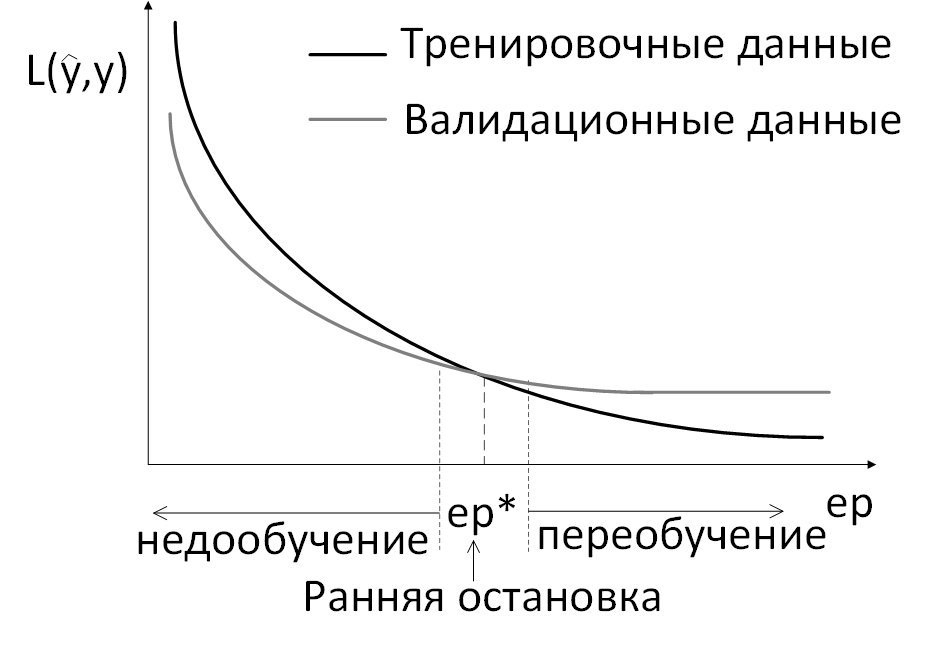
\includegraphics[width=0.75\linewidth]{./figuresch1/early_stop_cv.png}
		\caption{Иллюстрация зависимости ошибки обучения от эпохи для тренировочной и валидационной выборок, $ep^*$ - эпоха ранней остановки}		
		\label{ch1:fig:early_stop_cv}
	\end{center}
    \end{figure}
\end{itemize}

Работа \cite{lecun1998efficient} стало обобщением опыта по обучению нейронных сетей на момент ее написания. Многие из приемов, описанных в \cite{lecun1998efficient} используются в НС компьютерного зрения по настоящее время.

%%%%%%%%%%%%%%%%%%%%%%%%%%%%%%%%%%%%%%%%
\subsubsection{Регуляризация обучения нейронных сетей}
В работах 1989-1990 годов Погио и Гироси было показано, что точность работы нейронных сетей может быть повышена регуляризацией функции потерь при их обучении методом обратного распространения ошибки    \cite{poggio1989theory, girosi1995regularization}. Типичные техники регуляризации были предложены задолго до работа данных авторов. В том числе, наиболее популярная техника - гребневая регуляризация была предложена советским математиком А.Н. Тихоновым \cite{tihonov1963solution, tihonov1965rigeregr}. Данный тип регуляризации в наиболее простом виде часто называется \textbf{L2 регуляризация или регуляризация Тихонова}. По существу авторы работ \cite{poggio1989theory, girosi1995regularization} L2 регуляризацию к методу обратного распространения ошибки. По существу, задача обучения с регуляризацией соответствует введению дополнительного ограничения для оптимизируемых параметров (весовых коэффициентов):
\begin{equation}
\label{ch1:eqn:l2reg}
    \begin{cases} 
    L\left(y,\hat{y}(W,X)\right)\to \min 
    %     \\ 
    %   \hat{y}_i = f(\sum_{j=0}^{N-1} w_{ij}x_j)
        \\
    \sum_j w_j^2 \leq \mbox{const}
    \end{cases} 
    \Rightarrow 
    L\left(y,\hat{y}(W,X)\right) + \dfrac{\lambda}{2} \sum_j w_j^2 \to \min,
\end{equation}
где $ L\left(y,\hat{y}(W,X)\right)$ - функция потерь нейронной сети; $W=\{w_j\}$ - набор обучаемых весовых коэффициентов нейронной сети; $\lambda$ функция регуляризации. 
Использование регуляризации запрещает переобучаться нейронной сети за счет введения т.н. штрафа $\lambda$ в функцию потерь за слишком большую норму значений весовых параметров  ($\|W\|_2^2=\sum_j w_j^2$). Другими словами задача обучения из формулировки "функция потерь должна быть минимальной" превращается в формулировку "должен быть найден баланс между минимум функции потерь и максимум нормы значений весовых параметров". Заметим, что интуитивно понятно (и доказывается математически), что чем меньше значения весовых параметров тем меньше дисперсия (разброс) результатов - то есть выше обобщающая способность нейронной сети. Однако, можно также заметить, что введение регуляризации вводит смещение в функцию потерь, то есть выражение \ref{ch1:eqn:l2reg} ни когда не достигнет нулевых значений кроме как в тривиальном случае (когда все веса = 0, но этот случай нас не интересует). Таким образом, введение регуляризации вносит дополнительную ошибку в результаты обучения нейронной сети. Другими словами - принцип регуляризации - это компромисс между минимизацией дисперсии и смущением ошибки обучения нейронной сети. На практике 
значения $\lambda$ выбираются достаточно небольшими (порядка $10^-5 - 10^-6$), чего однако, часто хватает для необходимого повышения обобщающей способности без существенной потери точности работы нейронной сети.  
Отметим, что помимо L2 регуляризации в ряде случаев в нейронных сетях используется L1 регуляризация (LASSO) \cite{tibshirani1996regression} и комбинация L1 и L2 операций регуляризации \cite{ zou2005regularization}. Однако, именно L2 регуляризация является наиболее популярным среди аналогов \cite{moradi2020survey}. \textcolor{red}{Также в ряде источников семейство описанных методов регуляризации может называться weight decay.
Особенностях данных  и некоторых других типов регуляризации будут еще раз рассмотрены в книге в соответствующих разделах.  }

%%%%%%%%%%%%%%%%%%%%%%%%%%%%%%%%%%%%%%%%%%%%%%%%%%%
\subsubsection{Аугментация данных}
Существенно улучить результаты Лекуна удалось авторам работы \cite{simard2003best} 2003 года. Для этого авторами был предложен ряд техник расширения тренировочного набора данных путем искажений оригинальных экземпляров изображений - данная техника в настоящее время называется \textbf{Аугментация (augmentation - дополнение)}. Техники аугментации изображений были предложены в работе \cite{baird1992document} 1992 года, однако популярность обрели только после работы \cite{simard2003best}. Аугментация как правило выполняется путем аффинных (обратимых) искажений входных изображений или добавления к ним шумов или помех (например блики) \cite{ shorten2019survey}. Примеры результатов аугментации для изображения рукописной цифры приведены на рисунке \ref{ch1:fig:augumentation}. Отметим, что операцию аугментации следует выполнять с осторожностью. Мы рекомендуем начинать с обучения нейронной сети без аугментации, а затем постепенно увеличивая долю аугментированных данных следить за ошибкой на тестовых данных. Дело в том, что слишком интенсивной аугментацией можно изменить частоту встречи тех или иных признаков в данных или создать новые признаки. В современных нейронных сетях аугментация проводиться в процессе обучения нейронной сети случайным образом, что позволяет частично снизить вероятность появления описанных выше проблем. Отметим, что аугментация может быть рассмотрена как техника регуляризации нейронных сетей.

\begin{figure}[!h]
	\begin{center}
		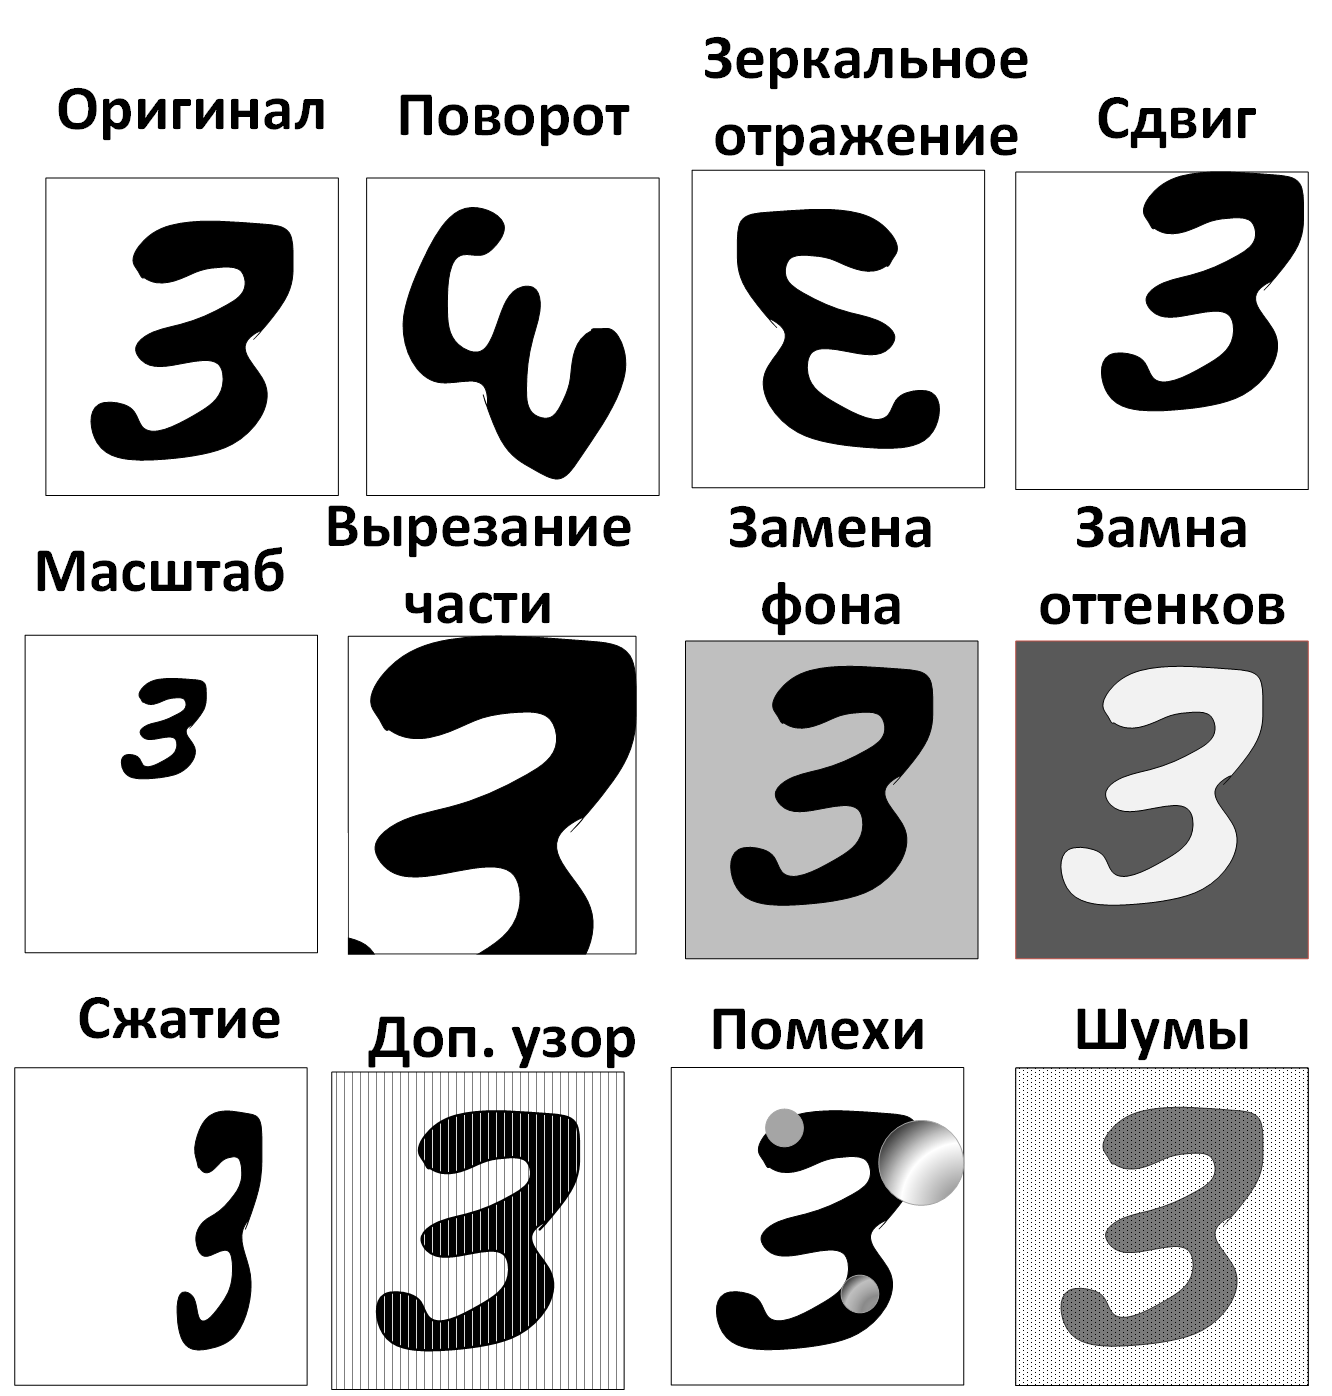
\includegraphics[width=0.6\linewidth]{./figuresch1/Augumentation.png}
		\caption{Иллюстрация примеров аугментации изображений для расширения входной выборки}		
		\label{ch1:fig:augumentation}
	\end{center}
\end{figure}
 

%TODO: надо описать еще термины обучение с учителем, без учителя и т.д.
%TODO: надо также во введении описать задачи КЗ решаемые с НС. в т.ч. классификация, объкты и тп - и сказать когда они возникли.
%TODO: надо сказать про overfit и что делать с ним
%TODO:НС или СНС - может ввести где-то?
%TODO:надо описать достоинства СНС в convnet1989 - инвариантность, в отличии от неокогн. меньше весовых парамертов, ?

%============================================%
\newpage
\subsection{Глубокие нейронные сети 2000-2012}
\subsubsection{Сети глубокого доверия, автокодирующие сети и метод жадного предобучения}
В середине 90-х и до 2005 (порядка 10 лет, не считая работ некоторых авторов) интерес к изучению нейронных сетей упал в силу технических ограничений вычислительной техники и проблемы вымывания градиента. Однако, например, по оценкам Лекуна \cite{lecun2015deep} в конце 90-х около 10\% чеков в банках США обрабатывались с использованием сверточных нейронных сетей.

В 2006 год Джефри Хинтоном была предложена техника предобучения нейронных сетей при помощи жадного послойного обучения \cite{hinton2006fast, hinton2007recognize}. Данный подход частично позволял избежать проблем выявленных ранее \cite{goodfellow2016deep}. 
В основе данной идее лежала архитектура нейронной сети - ограниченная машина Больцмана \cite{ackley1985learning, mcclelland1986parallel}, - архитектура предложена в 1986 г, полная машина Больцмана предложена в 1985 г. на основе т.н. сети Хопфилда (1982 г) (\cite{hopfield1982neural}) - подробное изложение данных архитектур выходит за рамки данной книги. 
В 2006 году ограниченная машина Больцмана была применена Хинтоном для решения задачи кодирования изображений (сжатие изображений) \cite{hinton2006reducing}. Данная архитектура нейронной сети в настоящее время известна как \textbf{автоэнкодер}. Отметим, что технически идея автокодерования была описана в 1987 в работе \cite{ballard1987modular} где была названа автоассоциативной сетью. Идея автокодирования в данной архитектуре основывалась на гипотезе о том, что многослойные нейронные сети позволяют выделять внутренние (закодированные) представления о регулярностях в данных (признаках) в окружающей среде (в обучающем наборе данных). Отметим, что также в работе \cite{ballard1987modular} была указана гипотеза о преимуществах иерархического (многослойного) кодирования входных данных  \cite{ballard1987modular}.

Типичная архитектура автоэенкодера представлена на рисунке \ref{ch1:fig:autoencoder}. Сеть стоит из двух частей:
\begin{itemize}
    \item часть 1: \textbf{энкодер} - сжатие входных данных - автоматическое выделение из них признаков. Принцип работы данной части аналогичен энкодеру признаков LeNet 5. Выход данного слоя часто называется \textbf{скрытым или латентным пространством (latent space).}
    \item часть 2: \textbf{декодер} - автоматическое восстановление данных из входных признаков (скрытого пространства).  
\end{itemize}
Сеть автоэнкодер обучается без учителя таким образом, что выходное изображение должно повторить входное. Ошибка воспроизведения минимизируется в ходе итерационного обучения. Выход обученного энкодера используется как кодирующая сеть. В случае необходимости закодированное изображение может быть восстановлено при помощи декодера.

\begin{figure}[!h]
	\begin{center}
		\includegraphics[width=0.86\linewidth]{./figuresch1/autoencoder_v2.png}
		\caption{Иллюстрация архитектуры автоэенкодера}		
		\label{ch1:fig:autoencoder}
	\end{center}
\end{figure}

Техника жадного послойного обучения представляет собой использование автоэнкодера для каждого слоя нейронной сети. 
Иллюстрация данного подхода приведена на рисунке \ref{ch1:fig:deep_belife_nn}.
Для первого слоя входными данными являются целевые входные данные НС. Результат предобучения первого слоя используется в качестве входных данных для предобучения второго слоя и т.д. Нейронные сети, предобученные методом жадного послойного предобучения часто называются \textbf{нейронные сети глубокого доверия.} \cite{goodfellow2016deep}. 

\begin{figure}[!h]
	\begin{center}
		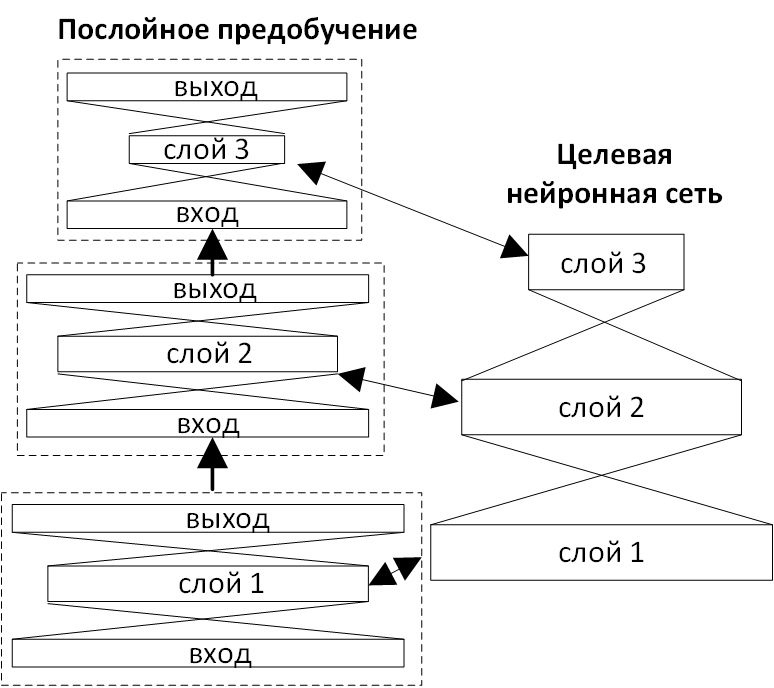
\includegraphics[width=0.76\linewidth]{./figuresch1/deep_belife_NN.png}
		\caption{Иллюстрация принципа жадного послойного предобучения (сети глубокого доверия)}		
		\label{ch1:fig:deep_belife_nn}
	\end{center}
\end{figure}

\uline{После предобучения (\textbf{pretrained}) НС должна быть дообучена (\textbf{fine tuning}) для решения целевой задачи}. Например, в  методом обратного распространения ошибки - в случае задачи обучения с учителем. 

Идея предобучения нейронных сетей заключается в ожидании того, что весовые параметры обученных сетей будут настроены таким образом чтобы максимально эффективно выделять характерные признаки из входных данных. При этом ожидается, что приблизительно те же признаки должна научиться выделять НС в ходе обучения так как признаками должны быть все наиболее регулярные особенности тренировочной выборки. Другими словами весовые параметры предобученной НС почти наверное позволяют использовать НС для решения целевой задачи. 
В работе 2010 года \cite{erhan2010does} на основании большого числа экспериментов авторами было показано, что использование предобучения нейронных сетей является методом регуляризации обучения нейронных сетей для целевой задачи. Также было показано, что использование предобучения НС повышает обобщающую способность и снижает дисперсию ошибок для тестовых данных. Другими словами снижается как ошибка на тренировочных данных, так и ее разность с ошибкой на тестовых данных, так и дисперсия ошибки на тестовых данных \cite{erhan2010does}. 

В 2007 году Й. Бенджо обобщил результаты Д. Хинтона и показал, что использование предобучения нейронных сетей позволят тренировать нейронные сети гораздо большей глубины \cite{bengio2007greedy}.
\textcolor{red}{
Также отметим, что Д. Хинтона, Й. Бенджио и Я. Лекуна на 2006 год работали совместно в рамках программы CIFAR NCAP} \cite{goodfellow2016deep}. 
В 2004-2006 годах в работах \cite{oh2004gpu, steinkraus2005using, chellapilla2006high} были показаны преимущества использования графических ускорителей (Graphic Process Unit, GPU)  при обучении сверточных нейронных сетей.
Фактически с описанных работ начинается 
\textbf{эпоха глубокого обучения нейронных сетей}.

\newpage
\subsubsection{Термин "Глубокое Обучение"}
%%%%%%%%%%%%%%% DEEP LEARNING
 Идея \textbf{глубокого обучения (Deep Learning) нейронных сетей} была высказана в работе Бенджо и Лекуном в работе \cite{bengio2007scaling}. В данной работе авторы авторы призвали сообщество исследователей методов машинного обучения к разработке алгоритмов, позволяющих максимально автоматизировать процесс выбора признаков, необходимых для решения задач. Также авторы показали, что необходимым условием выделения наиболее абстрактных признаков (высоко-уровнеаых признаков) является увеличение глубины нейронных сетей.  Для глубоких нейронных сетей было показано, что с увеличением глубины нейронных сетей возрастает их обобщающая способность. При этом обобщающая способность обусловлена нелинейностями в НС \cite{bengio2007scaling}.
\textcolor{gray}{
Также отмечается, что для сверхточных нейронных сетей все признаки являются пространственно локализованными. Признаки различных уровней образуют иерархию, в которой  локальные высокоуровнеые признаки формируются нелинейными комбинациями более низкоуровных локальных признаков.  \cite{lecun2015deep}.}

Отметим, что авторы \cite{bengio2007scaling} в противоположность глубокому обучению авторы понятие мелкого обучения (\textbf{shallow learning}) - нейронные сети с одним или небольшим количеством слоев. При этом, обещающая способность мелкой нейронной сети можно назвать локальной. Преимущества глубокой нейронной сети в этом случае можно обосновать обобщением большого количества локальных областей обобщения. Также авторами \cite{bengio2007scaling} была отмечена одна из основных проблем глубокого обучения - т.н. \textbf{"проклятие размерности"} как основного фактора, ограничивающего углубление нейронных сетей. Проклятие размерности заключается в экспоненциальном росте числа параметров слоя НС при линейном увеличении числа входов. Решение данной проблемы является одним из трендов развития НС по настоящее время. При этом авторами \cite{bengio2007scaling} была выдвинута гипотеза, что переход от однослойной архитектуры к многослойной позволяет сократить число параметров, необходимое для решения задачи. 

\textcolor{red}{
ГЛАВНОЕ ПРЕИМУЩЕСТВО DL; выделение, преобразование и выбор признаков, релевантные поставленной задачи. Однако процедура обучения требует достаточно большого набора данных для правильной обработки таких  признаков  }
\newpage
\subsubsection{Функция активации ReLU}
%%%%%%%%%%%%%%%%% RELU
В 2009-10х годах в работах \cite{jarrett2009best, nair2010rectified} было предложено использование ректифицированных функций активации вместо логистической функции активации и других вариантов функций с насыщением (ректифицированных - исправляющих, например операция модуль в качестве функции активации). Среди различных вариантов ректификационных функций наилучших результатов удалось добиться для функции \textbf{ректификационный линейный модуль (ReLU - rectified linear unit)}.
График функции ReLU и ее производной ReLU'(z) представлены на рисунке \ref{ch1:fig:relu}
Функция ReLU(z) и ее производная ReLU'(z) имеют следующий вид:

\begin{equation}
    \label{ch1:eqn:relu}
    \mbox{ReLU}(x)=\mbox{max$(0,x)$}, \ \ \ \mbox{ReLU}'(x) =
    \begin{cases}
        \mbox{$1$} & \mbox{if } x > 0\\
        \mbox{$0$} & \mbox{if } x \leq 0
    \end{cases}
\end{equation}

\begin{figure}[h]
	\begin{center}
		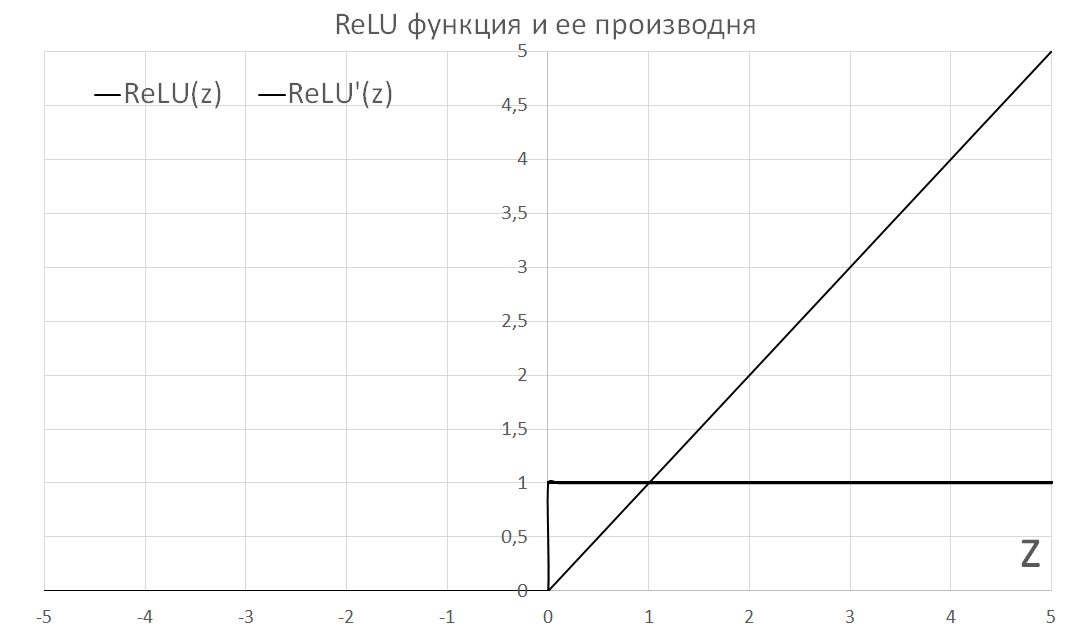
\includegraphics[width=0.75\linewidth]{./figuresch1/relu.png}
		\caption{график функции ReLU и ее производной}		
		\label{ch1:fig:relu}
	\end{center}
\end{figure}

\uline{Использование функции ReLU позволяет частично избежать проблем, связанных с  вымыванием градиента}. Так как функция не имеет насыщения в области $z>0$. При этом функция имеет низкую вычислительную сложность и позволяет обнулить часть весовых коэффициентов, что также может исключить часть вычислений (если один из параметров 0, то умножение на него можно не проводить). \uline{Функция ReLU является одной из наиболее популярных в настоящее время}. Как правило, нейронные сети с использованием ReLU показывают наилучшие результат среди других функций активации. Однако, потенциально у функции ReLU есть ряд недостатков, о которых будет сказано в свое время. Также следует отметить, что в настоящее время по мимо описанной реализации ReLU в литературе предложено семейство линейных и нелинейных модификаций этой функции активации, которые могут быть использованы если стандартной реализации недостаточно \cite{goyal2020activation}.
% Отметим, что в оригинальной работе \cite{nair2010rectified} предлагался вариант зашумленной ReLU $\mbox{ReLU}(x)=\mbox{max$(0,x+\N(0,\sigma))$}$, где $\N(0,\sigma)$ - нормальное распределение с 0 математическим ожиданием с дисперсией $\sigma^2$ однако, оказалось, что шумы не дают приемуществ.%


\subsubsection{Инициализация Весовых параметров}
%%%%%%%%%%%%% XAVIER
В 2009 году Хавьером Глори и Джефри Хинтоном было предложено в качестве альтернативы предобучению нейронных сетей проводить инициализацию их весовых параметров следующим способом, называемым \textbf{метод инициализации Хавьера (иногда называют инициализация Глори)} \cite{glorot2010understanding}:
\begin{equation}
    \label{ch1:eqn:xavier}
    W_i\sim U\left[-\frac{\sqrt{6}}{\sqrt{n_{i}+n_{i+1} }},\frac{\sqrt{6}}{\sqrt{n_{i}+n_{i+1}}}\right]
\end{equation}
где $U[a,b]$ - равномерное распределение со значениями от $a$ до $b$; $w_i$ is the weights of $i$-th layer, $n_{i}$, $n_{i+1}$ число входных параметров слоя с номером $i$ ($n_{i}$) и число выходных параметров ($n_{i+1}$). 
%% https://medium.com/@gidim/part-2-selecting-the-right-weight-initialization-for-your-deep-neural-network-cc27cf2d5e56
%% https://towardsdatascience.com/weight-initialization-in-deep-neural-networks-268a306540c0

Инициализация Хавьера основана на схеме инициализации Лекуна (\ref{ch1:eqn:lecun}). Однако, авторы \cite{glorot2010understanding} утверждали, что в оригинальной идеи Лекуна был проанализирован случай только прямого распространения ошибки. При получении выражения  \ref{ch1:eqn:xavier} было также учтено и обратное распространение ошибки. Авторами \cite{glorot2010understanding} утверждалось, что при инициализации весовых параметров вида \ref{ch1:eqn:xavier} вероятность переобучения достаточно сильно снижается. При этом авторами было обнаружено, что нейронные сети с логистическими функциями активации могут выходить из области насыщения в ходе обучения. Эксперименты авторов показали, что НС, с инициализацией весов \ref{ch1:eqn:xavier} имеет точность на тестовых данных выше, чем без инициализации, но ниже чем с пред обучением.

% \textcolor{red}{Также отметим, что в 2012 году была предложена архитектура глубокой стековой нейронной сети \cite{deng2012scalable}.В которой входными данными для каждого слоя являлись как выходные данные предыдущего слоя, так и входные данные нейронной сети, свернутые отдельным ядром. }
\uline{В 2015 году Каймингом Хе и соавторами из компании Microsoft был предложен метод инициализации функции ReLU}, позволявший обходить результаты, получаемые при помощи инициализации Хавьера Глори \cite{he2015delving}. В основе предложенного метода инициализации была положена идея учета несимметричного характера поведения функции  ReLU.  \textbf{Метод инициализации Хе (иногда называют инициализация Кайминга)}:
\begin{equation}
    \label{ch1:eqn:he}
    W_i\sim w_i\sim N\left[0 ,\frac{2}{n_i} \right]
\end{equation}

В настоящее время существует несколько вариантов выражений для инициализацией Хе и Глори, а также некоторых других, рекомендуемых для различных вариантов функций активации \cite{narkhede2021review}. Использование инициализации весов при отсутствии возможности или необходимости предобучения  нейронных сетей позволяет повысить обобщающую способность нейронных сетей, ускоряет процесс обучения и стабилизирует результаты их обучения (при повторениях процедуры).

%%%%%%%%%%%%%%%%%%%%%%%%%%%%
\subsubsection{Техники регуляризации методом Дропаут(DropOut)}

В 2012 году Джефри Хинтоном и соавторами, в том числе Алексом Крижевски, была опубликована работа, в которой авторы указали на одну из возможных интерпретаций переобучения и предложили решение данной проблемы - \textbf{т.н. метод дропаутов (dropping out, dropout)}\cite{hinton2012improving}. Авторами замечено, что в переобученной нейронной сети имеет место \textbf{проблема содаоптации (co-apadtation}  - это состояние обучения нейронной сети, когда нейроны каждого следующего слоя обучаются корректировать результаты работы нейронов предыдущего слоя. В Нормально обученной нейронной сети (не переобученной) предполагается, что каждый следующий слой нейронной сети работает независимо от предыдущего. То есть обучается выделять регулярные признаки из входных для него данных.  В переобученной нейронной нейрон перестает выделять регулярности и начинает подстраивать ответ под конкретные экземпляры входных данных, включая все их случайные и регулярные особенности \cite{hinton2012improving}. Другими словами нейронная сеть перестает работать как система с гибким статистическим выводом и превращается в аналог конечного автомата. 
В работе \cite{hinton2012improving} было предположено, что решениями проблемы со-адаптации могу быть использование нескольких нейронных сетей, каждая из которых обучена на части входных данных или реализация такой структуры внутри одной сети. Последний вариант предполагает, что в каждой эпохе обучения нейронная сеть не учитывает ряд случайных признаков (выходов нейронов для каждого слоя) в результатах работы слоя - \uline{этот метод называется - метод Дропаутов}. Число случайно выключаемых признаков как правило задается т.н. вероятностью дропаута $p$, который является гиперпараметром при обучении нейронной сети. Отметим, что метод дропаутов используется только при обучении нейронной сети. При ее работе все нейроны включены, а результат работы каждого нейрона должен быть домножен на $1-p$. Иллюстрация работы метода дропаутов во время двух разных эпох обучения для $p=0,33$ приведена на рисунке \ref{ch1:fig:dropout}. Отметим, что использование метода дропуатов требует увеличения общего числа параметров нейронной сети. Также метод увеличивает дисперсию результатов, поэтому как правило рекомендуется снизить скорость обучения и использовать варианты метода обратного распространения ошибки с моментом. Также метод дропаутов увеличивает общее время обучения нейронной сети в силу описанных особенностей. Следует отметить, что метод дропаутов используется после активационных функций. 
% По существу, метод дропаутов можно охарактеризовать как L0 регуляризация функции потерь, то есть регуляризация, стремящаяся уменьшить ошибку работы нейронной сети при условии минимума не нулевых элементов в сети. 
Несмотря на свои недостатки метод дропаутов в своих различных вариантах реализации остается одним из наиболее популярных методов регуляризации в нейронных сетях \cite{moradi2020survey, labach2019survey}. В 2013 году была опубликована работа \cite{baldi2013understanding}, посвященная математическому обоснованию работоспособности метода дропаутов. В работе \cite{baldi2013understanding} было показано, что метод дропаутов увеличивает обобщающую способность нейронной сети (регуляризирует обучение) и выполняет роль нормализации весовых параметров - то есть приводит их распределение к нормальному закону. Также в работе \cite{srivastava2014dropout} было экспериментально показано, что метод дропаутов может быть использован совместно с L2 и некоторыми другими типами классической регуляризации.

\begin{figure}[h]
	\begin{center}
		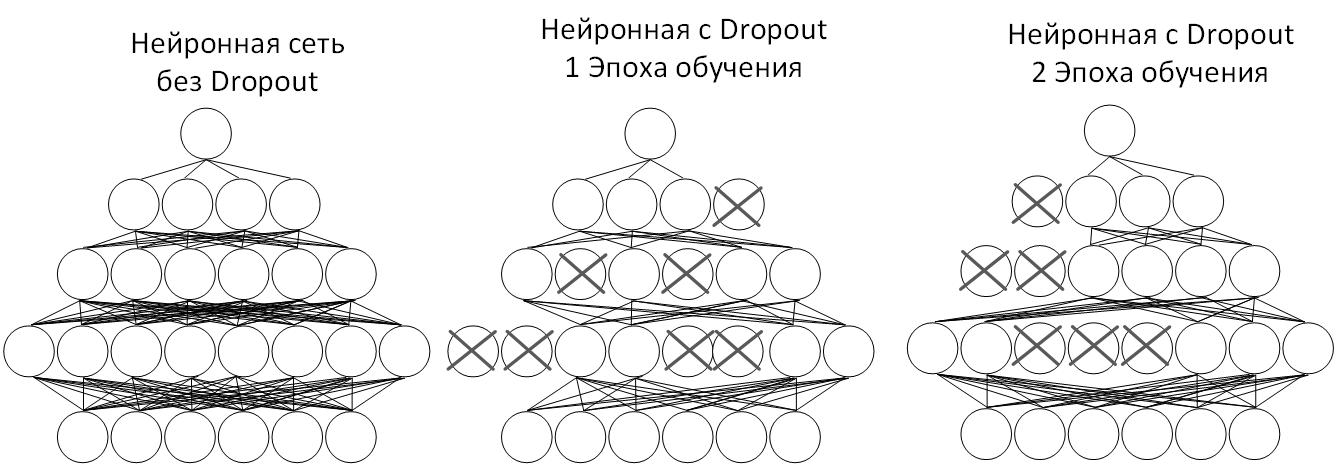
\includegraphics[width=0.79\linewidth]{./figuresch1/dropout.png}
		\caption{Иллюстрация работы метода дропаутов во время двух разных эпох обучения для $p=0,33$.}	\label{ch1:fig:dropout}
	\end{center}
\end{figure}

%%%%%%%%%%%%%%%%%%%%%%%%%%%%%%%%%%%%%%%%%%%%%
\subsubsection{Графические ускорители как основной инструмент обучения нейронных сетей}
Как уже было отмечено выше впервые преимущества использования графических ускорителей при обучении нейронных сетей были показаны в работах \cite{oh2004gpu, steinkraus2005using, chellapilla2006high}. Так в работе \cite{oh2004gpu} было заявлено 12-кратное ускорение обучения нейронной сети с использованием GPU по сравнению с обучением нейронной сети на центральном процессоре (ЦПУ) компьютера. Преимущества GPU заключаются в их возможности максимально быстро  выполнять перемножения векторов и матриц - то есть выполнять операции умножения с накоплением над одномерными и двухмерными массивами числе с плавающей запятой с высокой степенью параллельности. Отметим, что операция умножения с накоплением для чисел с плавающей запятой часто называется flop (float-point operation) большинство линейных операций (например $W^TX = \sum wx$) сводятся к операциями типа flop.

Обучение на GPU в 2004-2006 годах (в работах \cite{oh2004gpu, steinkraus2005using, chellapilla2006high}) представляло высокую сложность с точки зрения программного обеспечения. В силу технических ограничений существовавших на тот момент GPU разработка методов прямого прохождения через нейронную сеть и обратного распространения ошибки приходилось выполнять при помощи инструкций, предназначенных для расчета графических операций. В 2007 году компанией NVIDIA была представлен среда разработки под GPU CUDA (фреймворк CUDA), а также семейство графических ускорителей общего назначения (general purpose gpu, GPGPU). Использование CUDA и GPGPU позволило значительно упростить процесс разработки программного обеспечения для ускорения обучения нейронных сетей. Фреймворк CUDA имеет Си-подобный синтаксис и позволяет вести достаточно гибкую и быструю разработку программного обеспечения для графических ускорителей компании NVIDIA. Тенденция использования CUDA и GPU NVIDIA для обучения нейронных сетей сохраняется по настоящее время. Однако, сегодня разработчику не нужно осваивать непосредственно работу с CUDA - так как есть достаточно большое количество высокоуровневых фреймворков позволяющих компилировать код программного обеспечения как для CUDA (под GPU NVIDIA), так и для центральных процессоров (CPU). \uline{Большинство современных высокоуровневых фреймворков обучения глубоких нейронных сетей, в том числе для задач компьютерного зрения разработаны для языка программирования Python} \cite{nguyen2019machine}.

В 2010 и 2011 годах Киерсаном и авторами работ \cite{cirecsan2010deep, ciresan2011flexible} были описаны реализации глубоких полносвязной \cite{cirecsan2010deep}, и сверточной \cite{ciresan2011flexible} нейронных сетей, обученных на графических ускорителях (GPU) компании NVIDIA с использованием на тот момент, недавно представленного фреймворка разработки CUDA. Разработанные архитектуры нейронных сетей \cite{cirecsan2010deep, ciresan2011flexible} показали рекордные, на тот момент, точности для задач распознавания рукописных цифр (MNIST) и для набора цветных изображений 10 классов фотографий животных и техники (CIFAR-10 \cite{CIFARKrizhevsky2010}). Важно отметить, что в работах \cite{cirecsan2010deep, ciresan2011flexible}  нейронные сети обучались с использованием аугментации и без предобучения. Сверточная нейронной сеть основывалась на архитектуре LeNet 5, однако была значительно модифицирована, в частности, в ней слои усредняющей субдискретизации (average pooling) были заменены на слои maxpooling \cite{ciresan2011flexible}. 

Результаты Киерсана стали отправной точкой в разработке современных фреймворков глубокого обучения с использованием GPU. Одним из первых успешных фреймвороков разработки глубоких нейронных сетей с использованием GPU NVIDIA стало Tehano, представленное для языка программирования Python в 2010 году \cite{bergstra2010theano}. Фрейемровки типа Tehano значительно ускорили процесс развития глубокого обучения нейронных сетей. Во-первых такие фреймворки позволяют конечному пользователю не задумываться о тонкостях реализации низкоуровневых операций в нейронных сетях (например, свертка, варианты градиентного спуска или метод обратного распространения ошибки) - эти операции уже реализованы в фреймворке и запускаются "из коробки". Во-вторых конечному пользователю не нужно заботиться об особенностях запуска своего кода для конкретных аппаратных конфигураций, как правило фреймворки имеют свои реализации рассчитанные как для любых GPU компании NVIDIA, так и для произвольных CPU. В современных фреймворках также допускается использование графических ускорителей компании AMD - но в качестве эксперимента.  В-третьих, современные фреймворки предоставляют API (Application Programming Interface - интерфейс программного приложения) для языка Python \cite{li2020deep}. Данный язык программирования является одним из наиболее простых и высокоуровневых языков программирования, что позволяет освоить разработку нейронных сетей на Python практически любому, начиная со школьной скамьи.

Следует отметить, что набор CIFAR-10, а также его расширенная версия CIFAR-100 являются классическими наборами для тестирования и сравнения нейронных сетей (т.н. бентчмарков - benchmark) наборы разработаны Алексом Крижевски и представлены в работе Крижевски и Хинтона в 2010 году \cite{krizhevsky2010convolutional}. 

В 2011 году  Киерсан и его коллектив соавторов  показали наилучшие результаты в соревновании по распознаванию автомобильных знаков \cite{cirecsan2011committee} при помощи вышеописанной архитектуры вида \cite{ciresan2011flexible}. В том числе, авторы \cite{cirecsan2011committee} показали превосходство своей нейронной сети по сравнению с экспертами, также прежде не видевшими тестовый набор данных. При этом точность работы нейронной сети составила 1,02\%, эксперты смогли достичь точности в 1,19\% \cite {schmidhuber2015deep}. 

В 2012году Киерсаном и его коллективом было показано, что ансамбль нейронных сетей позволяет достичь точности эквивалентной человеку для рукописного набора цифр MNIST (погрешность 0,2\%) \cite{ciregan2012multi}. Отметим, что понятие \textbf{ансамбль нейронных сетей} означает, что используется структура из нескольких параллельно работающих нейронных сетей, результаты работы которых объединяются некоторым алгоритмом принятия конечного решения. Входные данные для такого алгоритма называются метаданными, а сам алгоритм мета-алгоритм. В качестве такого алгоритма может быть простое усреднение, выбор по большинству (голосование) или еще одна нейронная сеть - мета-сеть. Иллюстрация архитектуры ансамбля нейронных сетей приведена на рисунке \ref{ch1:fig:ensemble}. в работе \cite{ciregan2012multi} в качестве алгоритма использовалось простое усреднение, а каждая пара нейронных сетей имела свою пред обработку. Отметим, что ансамблевый подход к решению задач требующих презеционной точности характерен и в настоящее время. Как правило соревнования, подобные описанным выигрываются именно с использованием ансамблей нейронных сетей.

\begin{figure}[!h]
	\begin{center}
		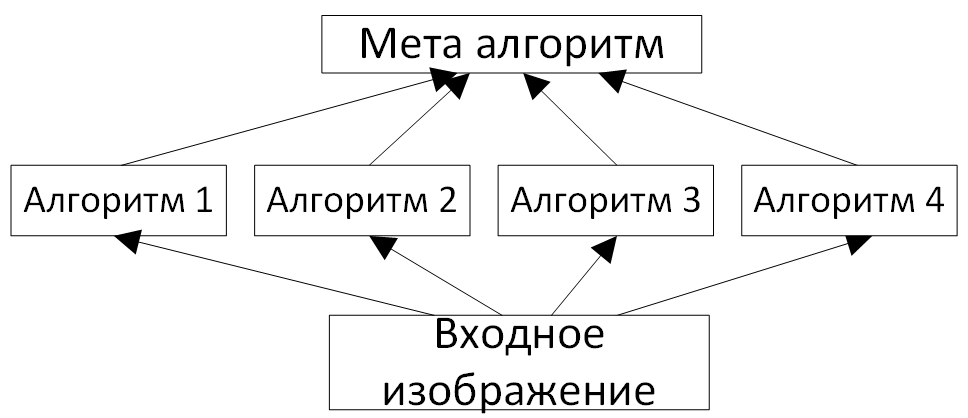
\includegraphics[width=0.7\linewidth]{./figuresch1/Ensemble.png}
		\caption{Иллюстрация архитектуры ансамбля нейронных сетей}		
		\label{ch1:fig:ensemble}
	\end{center}
\end{figure}

%%%%%%%%%%%%%%%%%%%%%%%%%%%%%%%%%%%%%%%%%%%%%
\newpage
\subsection{Экстенсивное развитие глубоких нейронных сетей 2012-2016 гг }
\subsubsection{ImageNet, GPU, Internet - катализаторы прогресса}
\textcolor{brown}{
%TODO: может это не надо?
В начале 21 века (в начале эпохи глубокого обучения) ключевыми тенденциями в глубоком обучении были:  возможность использования обучения без учителя и самообучения нейронных сетей, а также ключевая проблема статистического оценивая – высокое качество обобщения на новые данные после обучения на небольшом количестве примеров \cite{goodfellow2016deep}. Данные тенденции были смещены на второй план в 2010х. В это время в результате сильных прорывов в цифровизации технологий стали позволять проводить обучения НС на достаточно больших объемах данных. По крайне мере проводить предобучение на достаточно больших объемах данных. Этому способствовали как успехи в развитии GPU - вычислительной базы и развитии инструментов работы с GPU, так и успехи в развитии широкополосного доступа к сети интернет - то есть возможности сбор больших выборок данных для обучения. Тенденции 2010х привели к возможности углубления нейронных сетей и простоте работы с ними. Это в свою очередь привлекло внимание как научного так и инженерного сообществ и привело к гонке экстенсивного развития нейронных сетей.}

\uline{Одним из наиболее важных катализаторов интереса к развитию нейронных сетей стали соревнования  алгоритмов компьютерного зрения ImageNet Large Scale Visual Recognition Challenge  (ImageNet LSVRC, ILSVRC), запущенные в 2010 году}. Соревнования ILSVRC проводятся регулярно с 2010 года и основаны на тестовой части набора данных \textbf{ImageNet} \cite{imagenetcvpr09, ILSVRC15}. Набор данных ImageNet включал в 2012 году порядка 10 миллионов изображений в высоком разрешении, размеченных для задач классификации на 10 тысячи категорий. Для соревнований ILSVRC по классификации изображений использовалась тестовая выборки из набора ImageNet, включающие порядка 150000 изображений для 1000 категорий \cite{ILSVRC2012, ILSVRC15}. Отметим, что ILSVRC проводятся по нескольким номинациям, которые от года к году могут меняться \cite{ILSVRC15}. В 2012 году авторам работы \cite{krizhevsky2012imagenet} удалось достичь точности классификации изображений ILSVRC 84\%, тогда как в 2011 году точность была 75\% \cite{ILSVRC15}. В 2020 для набора данных ImageNet достигается точность $~ 1.2\%$ \cite{paperswithcodeImagenet}. \textcolor{red}{Важно отметить, что описанные выше цифры точности соответствуют т.н. \textbf{"top-5 accuracy"} - это метод оценивая при котором результат классификации считается правильным если он соответствует любому из 5 выходов нейронной сети, которые имеют наиболее высокую вероятность. Оценка точности в классическом понимании (ответ с максимальным значением вероятности - правильный) соответствует термину "top-1 accuracy". В 2012 году точность по top-1 была 64\%, в 2011 \% 51 \%, в 2020 91\% \cite{paperswithcodeImagenet}.}

Следует отметить, что ImageNet LSVRC являются наиболее престижными соревнованиями между алгоритмами компьютерного зрения по настоящее время. Хотя, набор ImageNet и не является уже наиболее крупным набором изображений \cite{prabhu2020large}. 
%%%%%%%%%%%%%%%%%%%%%%%%%%%%%%%%%%%%%%%%%%%
\subsubsection{Глубокие сверточные нейронные сети AlexNet и ZFNet}
\uline{В 2012 году Алексом Крижевски и коллективом со-авторов был выигран ILSVRC 2010 в категории классификация изображений. \cite{krizhevsky2012imagenet}.} 
Архитектура предложенной нейронной сети авторами работы \cite{krizhevsky2012imagenet}  принято называть AlexNet (2012 год). Архитектура состоит из 7 скрытых слоев (плюс один выходной), 5 из которых сверточные и два полоносвязных скрытых слоя и один полносвязный выходной слой.Иллюстрация архитектуры AlexNet приведена на рисунке \ref{ch1:fig:alexnet}. 

\begin{figure}[!h]
	\begin{center}
		\includegraphics[width=0.99\linewidth]{./figuresch1/AlexNet_v1.png}
		\caption{Иллюстрация архитектуры глубокой сверточной нейронной сети AlexNet}	
		\label{ch1:fig:alexnet}
	\end{center}
\end{figure}

\textbf{Особенности архитектуры AlexNet}, позволившие перейти к 7 слоям (от 5 в LeNet) были \cite{krizhevsky2012imagenet}:
\begin{itemize}
    \item использование функций активации ReLU в скрытых слоях;
    \item использование аугментации данных, в том числе все изображения сжимались до размеров $256\times 256$ из которых затем случайным образом выбирались патчи размером $224\times 224$ - т.н. случайный кроп (random crop)- один из наиболее популярных видов аугментации по настоящее время; а также проводилось изменение интенсивности цветовых каналов входных изображений (входные изображения были в формате RGB - красный, зеленый и синий каналы). 
    \item использование обучения стохастическим пакетным градиентным спуском с моментом и L2 регуляризацией;
    \item регуляризация методом дропаутов с вероятностью 50\%;
    \item обучение на нескольких GPU при помощи параллельной обработкой групп каналов свертки - т.н. групповая свертка, когда все каналы $C$ (см. рис \ref{ch1:eqn:conv_3d_4d}) разделяются на группы и затем объединяются.
    % % TODO: возможно это тут не надо - так как не стало традицией.
    % \textcolor{gray}{ 
    % \item использование операции \textbf{локальной нормализация отклика фильтров (local response normalization, LNR};
    % \item использование операции субдискретизации с перекрытием.}
\end{itemize}
\textcolor{red}{Все перечисленные выше техники будут более подробно рассмотрены в соответствующих разделах книги.}\textcolor{brown}{
Отметим, что по мимо выше приведенных операций инновационными в архитектуре стали: использование операции субдискретизации с перекрытием и использование локальной нормализация отклика фильтров (local response normalization, LNR) для предотвращения взрывного роста весов \cite{krizhevsky2012imagenet} - однако, данные типы операций не стали классикой глубоких архитектур нейронных сетей.}

\uline{Архитектура AlexNet стала одним из наиболее значимых прорывов в области развития глубоких нейронных сетей}. Архитектура AlexNet была первой  одержавшей победу на соревнованиях ImageNet, более того, архитектура показала погрешность почти в 2 раза ниже, чем классические алгоритмы. Начиная с архитектуры AlexNet у научного и инженерного сообщества отпали сомнения в том, каким должен быть подход к решению задач компьютерного зрения. Начиная с 2012 года и по настоящее время подавляющее большинство задач компьютерного зрения решаются только методами глубокого обучения нейронных сетей \cite{Tsang2020Summary}. Также работа \cite{krizhevsky2012imagenet} задала направления развития глубокого обучения сверточных нейронных сетей. 

В 2013 победу на соревнованиях ILSVRC одержала модифицированная архитектура AlexNet - т.н. \textbf{ZFNet} \cite{zeiler2014visualizing}. Авторы работы \cite{zeiler2014visualizing} увеличили долю аугментации данных; провели предобучение на нескольких наборах данных, схожих с ImageNet; а также предложили метод визуализации работы слоев нейронной сети. Благодаря визуализации авторам работы  \cite{zeiler2014visualizing} удалось выбрать гиперпараметры архитектуры улучшающие точность работы нейронной сети\textcolor{brown}{. Также метод LNR было предложено заменить на метод локальной нормализации контраста (local contrast normalization, LCR)} \cite{zeiler2014visualizing}.

%%%%%%%%%%%%%%%%%%%%%%%%%%%%%%%%
\subsubsection{Расширение концепции сверточного слоя в 2012-2014 годах}
До 2014 года концепция сверточного слоя глубокой нейронной сети оставалась почти без изменений с работ Лекуна 1989 года. Хотя за этот период были измены функция активации, к слою были добавлены слой пулинг, были предложены некоторые методы регуляризации. 

В 2014 авторами коллектива  Visual Geometry Group (VGG) был предложен метод сокращения числа параметров свреточного слоя - \textbf{каскадная свертка}. uline{Идея каскадной свертки, заключается в замене одной свертки со сравнительно большим размером ядра (например $7\times 7$) на последовательное соединение нескольких небольших сверточных ядер, описывающих тот же размер рецептивного поля (например 3 свертки $3\times 3$)} \cite{simonyan2014very}. Это позволило авторами работы \cite{simonyan2014very} предложить ряд значительно более глубоких архитектур сверточных нейронных сетей, имеющих от 11 до 19 слоев (VGG-11, VGG-13, VGG-16, VGG-19). Архитектуры VGG-19 и VGG-16 показали точности 92\% и 91,4\% соответственно по "top-5 accuracy" на ILSVRC-14.  Архитектура VGG-16 используются по настоящее время в силу простоты. Однако, по соотношению числа параметров к точности она являются одной из наименее эффективных среди современных архитектур \cite{paperswithcodeImagenet}. 

%TODO: ADD VGG LAYER AND VGG-16 HERE

В 2013 Лин и соавторы опубликовали работу \cite{lin2013network}, в которой работе были предложены следующие приемы оптимизации сверточных нейронных сетей, ставшие впоследствии классическими.
\begin{itemize}
    
    \item \textbf{Концепция расширения понятия сверточный слой до понятия "сеть в сети" (Network In Network, NIN)}. Лином предложена архитектура слоя как последовательного соединения свертки и полносвязной сети, входы которой канальные выход операции свертки (см. выражение \ref{ch1:eqn:conv_3d_4d}). Основная идея "сеть в сети" заключается в увеличении числа нелинейностей (активационных функций) в каждом слое - соответственно увеличении возможностей для выделения нелинейных признаков каждым слоем нейронной сети. Сами авторы работы предлагали интерпретацию своей концепции как микросети, скользящей по входному изображению.
    
    \item \textbf{Использование глобального усредняющего пулинга (global average pooling, GAP)} вместо слоев векторизации набора полносвязных слоев в головной части нейронной сети. Основная идея глобального пулинга заключается в устранении набора полносвязных слоев, необходимых в случае векторизации, соответственно число параметров сети значительно снижается без существенных потерь в точности. Это делает обучение нейронных сетей более простым и снижает вероятность переобучения.
    
    \item \textbf{Использование точечной свертки ($1\times 1\times C$ - pointwise convolution) для выделения межканальных признаков}. Точечная свертка одна из наиболее часто используемых операций. Она позволяет сжимать или увеличивать число каналов в каждом сверточном слое - что позволяет варьировать число каналов и число выделяемых ими признаков.
    
\end{itemize}

Сам по себе подход Network In Network, предложенный авторами работы \cite{lin2013network} не получил широкой популярности. Однако, \uline{идея использования "сети в сети" легла в основу архитектуры\textbf{ GoogleInception V1 (GoogLeNet V1)}}, предложенной компанией Google (коллектив авторов во главе с Кристианом Седжеди) в 2014 году \cite{szegedy2015going}. 

Авторы работы \cite{szegedy2015going}(GoogLeNet V1) переработали концепцию NIN, расширили каждый слой до нескольких параллельных сверток и использовали для каждой свертки дополнительно свертку $1\times 1$ для регулирования общего числа параметров сети. Иллюстрация типичной архитектуры слоя сети GoogLeNet V1 приведена на рисунке \ref{ch1:fig:inception_layer}. Отметим, что в работе \cite{szegedy2015going} были также предложены использование промежуточных слоев принятия решений и метод аугментации для предобучения нейронных сетей наложением разных экземпляров данных  и их меток. Архитектура GoogLeNet V1 включала 22 слоя и показала точность 93,3 \% на ILSVRC 2014. В последующие несколько лет Кристианом Седжеди с соавторами были предложены несколько модифицированных вариантов архитектуры Inception \cite{szegedy2016rethinking, szegedy2017inception}. \textcolor{brown}{Данное семейство архитектур будет рассмотрено в книге более подробно.}

%TODO: возможно следует добавить слой NIN, хотя с другой стороны он не имеет практической ценности.
\begin{figure}[!h]
	\begin{center}
		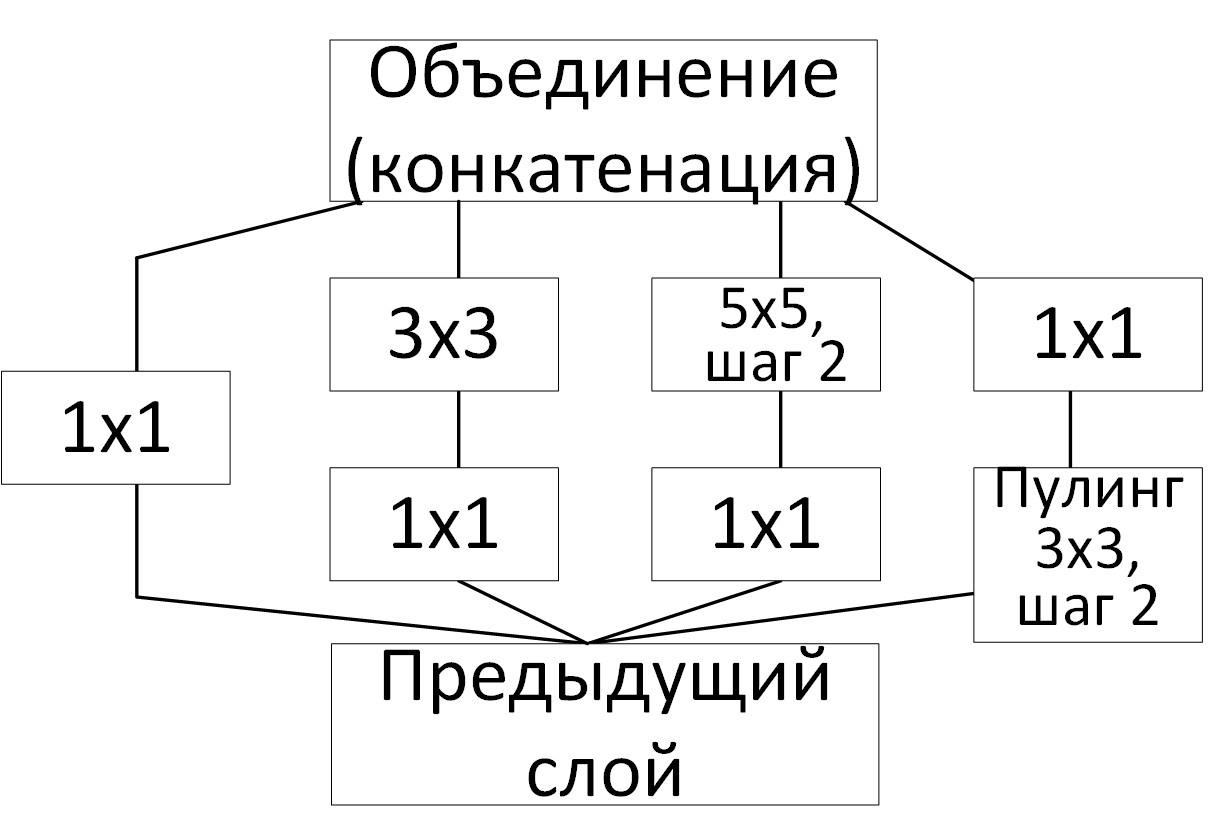
\includegraphics[width=0.5\linewidth]{./figuresch1/inception_layer.png}
		\caption{Иллюстрация типичной архитектуры слоя сети GoogLeNet V1}		
		\label{ch1:fig:inception_layer} 
	\end{center}
\end{figure}

Отметим, что расширение концепции сверточного слоя не ограничивается отмеченными выше работами. Скорее они являются лишь началом на этом пути \cite{khan2020survey}. В последующих разделах будет показано, как к данной концепции будут добавлены пакетная нормализация, тождественные связи, механизм внимания и другие приемы, позволяющие значительно повысить обобщающую способность и точность нейронных сетей. \textcolor{red}{Подробное исследование сверточных слоев будет проведено в последующих главах книги}.

%%%%%%%%%%%%%%%%%%%%%%%%%%%%%%%%%%%%%%%
\subsubsection{Пакетная нормализация (BatchNorm) }
В 2015 году Сергеем Иоффе и Кристианом Седжеди была предложена \textbf{техника пакетной нормализации - батчнормализации ( batch normalization, batchnorm, \textcolor{red}{технически будет правильней назвать межпакетная нормализация})} \cite{ioffe2015batch}. 

\uline{Идея метода батчнормализации заключалась в следующем}. Как правило обучение нейронной сети проводится методом стохастического пакетного градиентного спуска, то есть не по всей тренировочной выборке а по случайным подвыборкам - мини пакетам. Различия статистических характеристик между такими мини пакетами замедляет обучение нейронной сети и повышает требования к точности подбора гиперпараметров и требования к инициализации весовых параметров - то есть повышает вероятность переобучения и снижает обобщающую способность. Под статистическими характеристиками авторы понимают в первую очередь среднее и дисперсию по каждому признаку для каждой подвыборки (мини-пакета) входных данных. Описанный эффект авторы назвали \textbf{внутренний ковариационный сдвиг, internal covariate shift}. Для решения проблемы ковариационного сдвига в работе \cite{ioffe2015batch} было предложено использование нормализации результатов работы каждого слоя нейронной сети. При этом статистические характеристики должны усредняться по всем мини-пакетам и использоваться при работе обученной нейронной сети \cite{ioffe2015batch}. Математически батч-нормализацию можно выразить следующим образом:
\begin{equation}
    \begin{split}
    \label{ch1:eqn:BN}
   \hat y_i = f(\tilde{z_i}); \ \ \tilde{z_i} = \gamma\dfrac{z_i-\mu}{\sqrt{\epsilon+\sigma^2}}+\beta, 
    \\
    \mu_{\mathrm{TEST}} = \alpha  \mu_{\mathrm{TEST}} + (1-\alpha) \mu
    \\
    \sigma_{\mathrm{TEST}} = \alpha  \sigma_{\mathrm{TEST}} + (1-\alpha) \sigma
    \end{split}
\end{equation}
где 
\begin{itemize}
\itemsep 0.1em 
    \item $\hat y_i$ - результат работы нейрона;
    \item $f(\cdot)$ - функция активации; 
    \item $\tilde{z_i}$ - нормализованный линейный выход;
    \item $z_i$ - линейный выход (например $z_i = W^TX_i$);
    \item $\gamma, \beta$ - коэффициенты масштабирования (обучаются во время тренировки нейронной сети);
    \item $\mu = \dfrac{1}{N}\sum_{i=0}^{N-1} z_i$ - среднее по минипакету, \newline $N$ - размер минипакета (используется при обучении);
    \item $\sigma = \dfrac{1}{N}\sqrt{\sum_{i=0}^{N-1}(z_i^2 - \mu)^2}$ - среднеквадратическое отклонение по минипакету (используется при обучении);
    \item $\epsilon$ - константа для предотвралщения деления на 0;
    \item $\mu_{\mathrm{TEST}},  \sigma_{\mathrm{TEST}}$ - значения среднего и среднеквадратического отклонения, которые будут использоваться вне обучения нейронной сети;
    \item $\alpha$ - коэффициент сглаживания экспоненциальным средним при обновлении $\mu_{\mathrm{TEST}},  \sigma_{\mathrm{TEST}}$.
\end{itemize}
Из выражения  (\ref{ch1:eqn:BN}) и пояснений к нему могут быть сделаны следующие заключения касательно батчнормализации.
\begin{itemize}
\itemsep 0.125em 
    \item Операция батчнормализации по разному работает при обучении и в основном режиме работы нейронных сетей. 
    \item При обучении нейронных сетей в выражении (\ref{ch1:eqn:BN}) используются значения $\mu и \sigma$, вычисленные для текущего минипакета. 
    \item Значения коэффициентов $\gamma$ и $\beta$ обучаются во время тренировки и фиксируются в рабочем режиме нейронной сети.
    \item В рабочем режиме нейронной сети в выражении (\ref{ch1:eqn:BN}) используются значения $\mu_{\mathrm{TEST}}$ и $\sigma_{\mathrm{TEST}}$, вычисленные входе обучения.
    \item \uline{Операция батчнормализация должна быть использована перед активационной функцией}.
    \item \uline{Операция батчнормализации сводится к тому, что каждый пакет приводится  по каждому признаку: сначала к среднему 0 ($\mu$) и дисперсии 1 ($\sigma^2$), а затем масштабируется ($\gamma$) и смещается ($\beta$). По задумке авторов смещение и масштаб должны быть таковыми, чтобы результат нормализации ( $\tilde{z_i}$) всегда оказывался в "правильном" диапазоне значений для активационной функции}. Например, для логистической функции желателен диапазон $\tilde{z_i}\sim 0,6-0,8$, для функции ReLU $\tilde{z_i}>0$ и т.д. При этом так как параметры $\gamma$ и $\beta$ обучаются, сеть должна сама выбрать нужный диапазон значений $\tilde{z_i}$.
    \item Поскольку набор параметров $\mu, \sigma, \gamma, \beta$ одинаков для всех минибачей, следует ожидать одинакового поведения нейронной для каждого из них. Это снижает вероятность изменения ошибки работы нейронной сети в силу того, что установленные гиперпараметры больше подходят для одного минипакета и меньше подходят для дорого. \uline{Данное обстоятельство можно считать регуляризацией работы нейронной сети.}
\end{itemize}
Благодаря описанным выше особенностям метод батч нормализации стал одним из наиболее популярных методов регуляризации обучения нейронных сетей. После выхода работы \cite{ioffe2015batch} многими авторами были предложены различные вариации данного метода, а также ряд альтернативных вариантов нормализации (например нормализация весовых параметров) \cite{moradi2020survey, huang2020normalization, summers2019four}. \textbf{Недостатками классической версии (\ref{ch1:eqn:BN})} являются: чувствительность метода к изменению размера пакета; снижение регуляризационных свойств при небольшом размере пакета. \uline{Для корректной работы батчнормализации рекомендуется использовать пакеты от $~50-100$ экземпляров данных} \cite{zhang2021dive}. Использование метода батчнормализации будет более подробно рассмотрена в соответствующем разделе книги. 

Отметим, что в оригинальной работа \cite{ioffe2015batch} были представлены лишь интуитивные пояснения касательно того почему метод батчнормализации работает. Позже рядом авторов были предприняты попытки формального математического обоснования метода. Однако, общего результата нет по настоящее время \cite{lubana2021beyond, luo2018towards}. Также следует отметить, что батчнормализация на практике редко используется совместно с методом дропаутов. Дискуссия касательно обобщающих свойств обоих методов и рекомендаций к их использованию также остается открытой \cite{li2019understanding, zhang2021dive}. 

%%%%%%%%%%%%%%%%%%%%%%%%%%%%%%%%%%%%
\subsubsection{Слой остаточного обучения (residual layer)}
В 2015 году Каймингом Хе и соавторами (компания Microsoft) было предложено использовать \textbf{принцип идентичных связей} для обучения нейронных сетей увеличенной глубины. По задумке автора \uline{идентичные связи должны быть параллельны основному слою нейронной сети} \cite{he2016deep}. 
Слой (или бок слоев) нейронной сети с идентичными связми принято называть \textbf{skip-connection, identity-connection, residual-connection или residual-layer, остаточный слой, тождественный слой}. Иллюстрации остаточного блока нейронной сети без остаточного слоя, аналогичного блока с остаточным слоем \cite{he2016deep} и блока с модифицированным остаточным слоем \cite{he2016identity} (2016 г., Каймингом Хе и соавторы) приведены на рисунках \ref{ch1:fig:residual_layer} А), Б) и В) соответственно.

\begin{figure}[!h]
	\begin{center}
		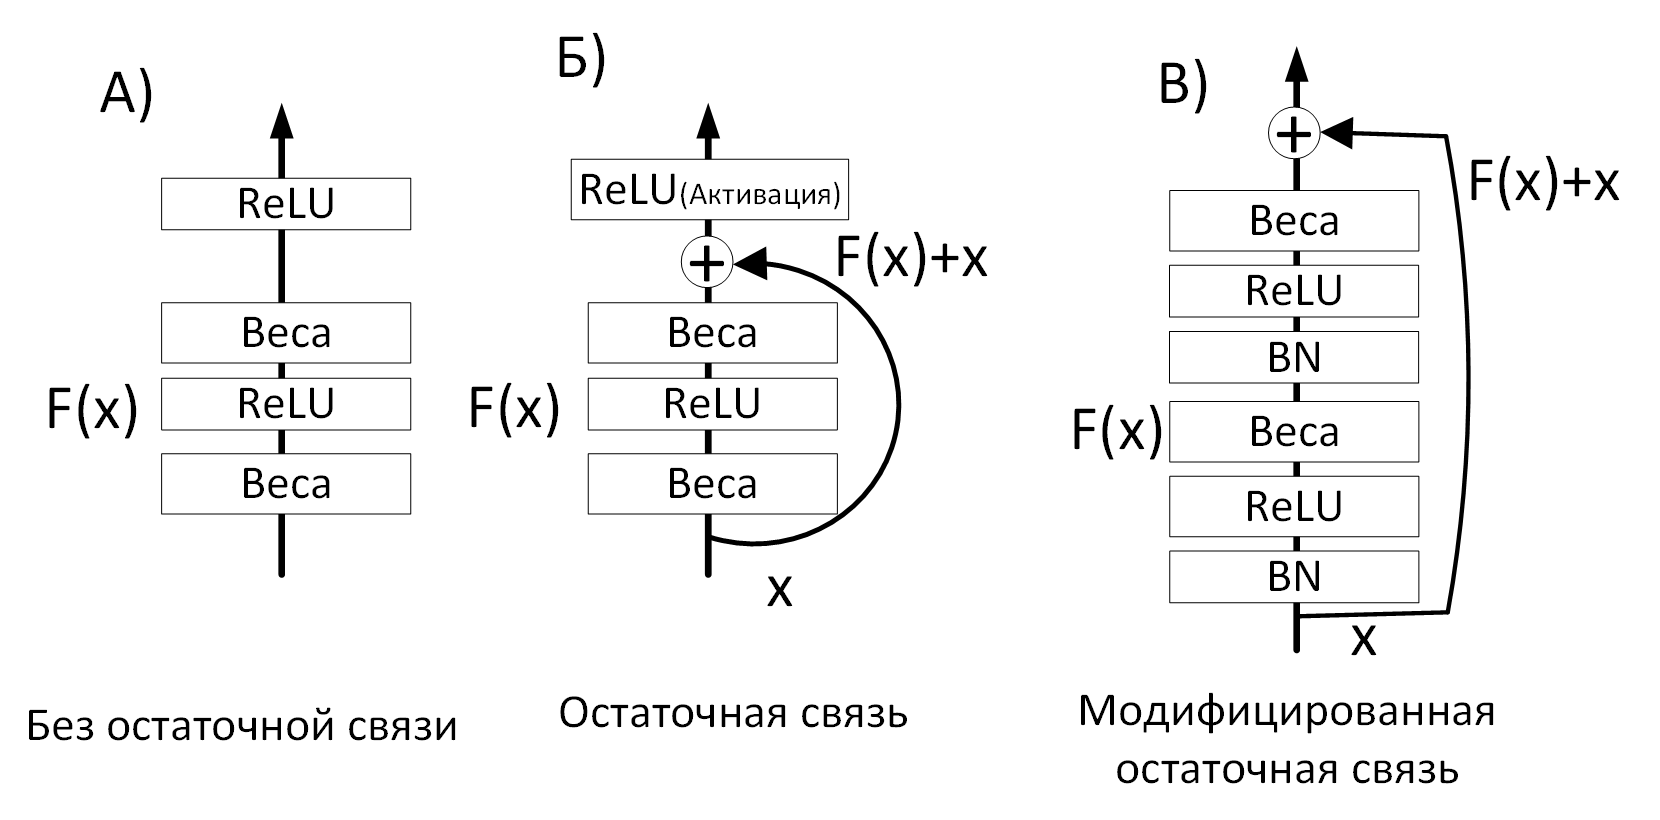
\includegraphics[width=0.99\linewidth]{./figuresch1/residual_con_v1.png}
		\caption{Иллюстрация слоя с остаточной связью: А) блок слоев без остаточной связи; Б) блок с остаточной связью; В) блок с модифицированной остаточной связью}		
		\label{ch1:fig:residual_layer}
	\end{center}
\end{figure}

Благодаря использованию остаточной связи (см. рис \ref{ch1:fig:residual_layer} Б) авторами работы  \cite{he2016deep} удалось увеличить глубину нейронных сетей до 152 слоев. Архитектуры сверточных нейронных сетей с остаточными связями, разработанных авторами \cite{he2016deep} принято называть ResNet-18, ResNet-34, ResNet-50, ResNet-101, ResNet-152, где цифра обозначает число слоев. В соревнованиях ILSVRC 2015 модель ResNet-152 достигла погрешности 4,6\% для одной сети и 3,6\% для ансамбля сетей \cite{he2016deep}. При этом значения ошибки ниже, чем для эксперта (у человека ошибка для тех же условий порядка 5 \% \cite{alom2019state}).

\uline{В основе работы остаточных связей лежат следующие идеи}. Если во время тренировки нейронной сети в основном слое или блоке слоев возникает вымывание или взрыв градиента, то остаточная связь действует как регуляризация, компенсируя проблему. Компенсация происходит за счет суммирования информации (входных данных) перед блоком и результата работы самого блока. В случае, если блок не нужен нейронной сети (например слишком глубокий слой), то по задумке авторов сеть должна обучиться так, чтобы влияние остаточной связи преобладало в блоке \textcolor{red}{(говоря на языке электронной схемотехнике - шунтировало блок)}. Таким образом остаточная связь является приемом регуляризации обучения нейронных сетей. Благодаря остаточным связям стало возможным увеличивать глубину нейронных сетей практически до бесконечности. 

В 2016 году Каймингом Хе и соавторами была опубликована работа \cite{he2016identity} в которой авторы смогли увеличить глубину сети ResNet c 152 до 1001 слоя, благодаря разработке модифицированной версия блока с остаточными связями (рис. \ref{ch1:fig:residual_layer} В). При этом оказалось, что точность на наборе данных CIFAR-10 увеличилась лишь с 5,46 \% до 4,62 \% \cite{he2016identity}. Данный результат можно объяснить тем, что в результате обучения сети большинство слоев выше 100-200 полностью или почти полностью представляют собой остаточную связь - то есть не нужны. 
\textcolor{red}{
Также отметим, что в 2016 году в работе \cite{huang2016deep} была опубликована архитектура рекордно глубокой сети, имеющей 1202 слоя. Сеть был обучена используя прием дропаута слоев (т.н. стохастическая глубина), что, позволило несколько увеличить точность но оставило вопрос об эффективности такой архитектуры (в отношении точность/время/вычислительные ресурсы) открытым.}

\uline{Эксперименты проведенные Каймингом Хе и соавторами в работах} \cite{he2016deep, he2016identity} \uline{показали сообществу исследователей нейронных сетей, что увеличение возможностей нейронных сетей за счет их углубления не является бесконечным и заставило задуматься о других  путях совершенствования нейронных сетей}. В 2016 году сообщество исследователей нейронных сетей начало работать на увеличением ширины слоя нейронных сетей при фиксированном числе слоев, а затем перешло к оптимизации каждого слоя. Так, в соревнованиях ILSVRC 2016 второе место с отрывом в 0,04\% одержала архитектура ResNeXt - вариант архитектуры ResNet c оптимизированной структурой блока \cite{xie2017aggregated}. При этом первое место занял ансамбль из набора известных архитектур, не внесший существенного вклада в развитие методов глубокого обучения\cite{Tsang2018Trimps}. 
\textcolor{red}{Подробно архитектуры на основе ResNet будут рассмотрены в соответствующем разделе книги}.

%%%%%%%%%%%%% DENSE NET %%%%%%%%%%%%%%%%%%%%%%%%%
Среди различных вариантов реализации идеи остаточного слоя в данном разделе хочется отметить работу 2017 года \cite{huang2017densely}. В данной работе было предложено расширить понятие блока с остаточными связями до вида, который принято называть \textbf{DenseNet}. Иллюстрация блока DenseNet приведена на рисунке \ref{ch1:fig:densenet}. По существу,  архитектура DenseNet может быть классифицирована как отдельный класс сверточных нейронных сетей. Идея блока DenseNet заключается в организации набора остаточных связей таким образом, что информация с каждого слоя блока DenseNet добавляется к результату последующего блока. При этом такое добавление информации происходит без соответствующего увеличения числа параметров, что позволяет обойти т.н. проблему проклятия размерности \textcolor{red}{о которой говорилось выше}. Таким образом, \uline{не смотря на большое число признаков в каждом из слоев, общее число параметров в блоке DenseNet остается небольшим}, что дополнительно снижает вероятность переобучения нейронной сети и ускоряет ее обучение. Благодаря использованию блока DenseNet авторам работы \cite{huang2017densely} удалось создать архитектуру с числом слоев от 121 до 264. При этом данные архитектуры имели точности сопоставимые с классическими моделями ResNet c тем же числом слоев, однако при этом в архитектурах DenseNet число параметров было в 3-10 раза ниже \cite{huang2017densely}.

\begin{figure}[!h]
	\begin{center}
		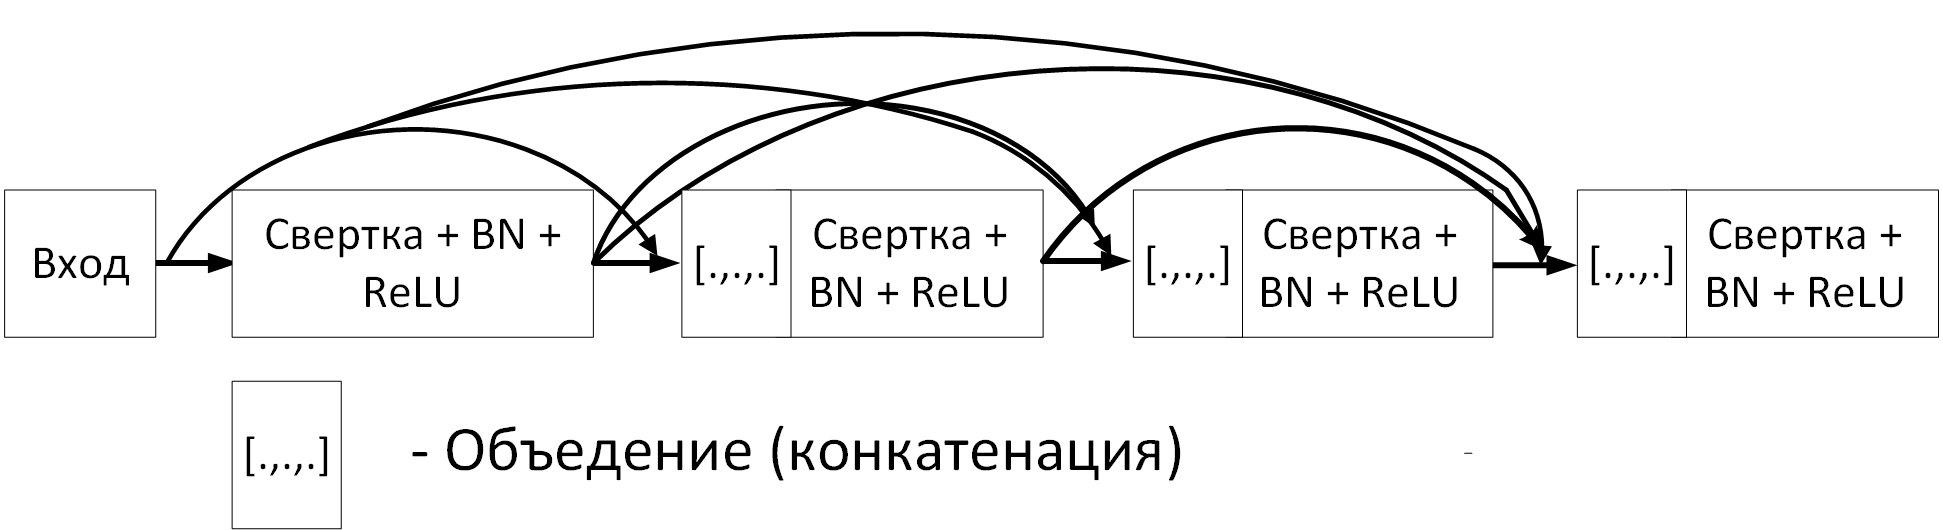
\includegraphics[width=0.99\linewidth]{./figuresch1/densenet.png}
		\caption{Иллюстрация блока DenseNet c остаточными связями}		
		\label{ch1:fig:densenet}
	\end{center}
\end{figure}

\uline{Идея использование остаточной связи стала революционной в сверточных нейронных сетях, практически все последующие работы, предлагающие новые архитектуры сверточных и полносвязных нейронных сетей содержали остаточные связи в различных вариантах} в рамках кодировщика признаков (feature encoder) \cite{khan2020survey}. 

%%%%%%%%%%%%%%%%%%%%%%%%%%%%%%%%%%%%%%%%%%%%%%%%%%%%%%%%%%%
\newpage
\subsection{Современное состояние глубоко обучения в задачах компьютерного зрения}
\subsubsection{Мобильные сверточные архитектуры 2016-2017}
Как уже было отмечено выше с 1989 до 2016г основным направление развития сверточных нейронных сетей было поиск путей их углубления. В том числе, эта тенденция была связана с ростом возможностей серверной вычислительной техники которая подразумевалась в основных приложениях компьютерного зрения. Однако, к 2016 году успех глубокого обучения сверточных нейронных сетей все с большей интенсивностью открывали вопрос об их использовании в низко-производительных ( в т.ч. мобильных) вычислительных устройствах. \uline{К этому моменту уже были предложены ряд техник по сжатию (компрессии) обученных нейронных сетей для их реализации в конечных устройствах \cite{mishra2020survey}. Были предложены и специализированные архитектуры аппаратных ускорителей для нейронных сетей \cite{reagen2016minerva}}. Однако, процесс компрессии и ускорения не позволял изначально обучить модель с требуемым размером. То есть для экспериментов с обучением нейронных сетей все равно требовались высокопроизводительные серные вычислительные устройства и высокие временные затраты. 

%%%%%%%%%%%%%%% SQUEEZE NET %%%%%%%%%%%%%%%%%
\uline{В 2016 году для решения проблемы мобильных архитектур авторами работы \cite{iandola2016squeezenet} была предложена архитектура нейронной сети, обладающей производительностью на уровне AlexNet (см. выше) при числе параметров в 50 раз ниже (5 МБайт против 240 у AlexNet)}. Архитектура сети была названа \textbf{SqeezeNet}.Основные идеи SqeezeNet заключались в следующем.
\begin{itemize}\itemsep 0.25em  
    \item Замена части традиционных сверток на свертки 1х1 (точечные свертки) - что снижает число параметров, например в случае свертки $3\times3$ снижает в 9 раз.
    \item Использования слоя сокращения числа карт признаков перед сверткой (сжимающий слой, sqeeze layer). Предполагается, что не все карты признаков необходимы для конечного результата. В ходе обучения нейронная сеть должна научиться оставлять только не обходимые карты. Интуитивно данный принцип следует из предположения, что в правильно обученной нейронной сети каждый слой работает независимо от последующих слоев.
    \item Реализация субдискретизации (пулинга) ближе к оконечным слоям нейронной сети. По мнению авторов и результатам работы Кайменга Хе такой подход позволяет иметь карты признаков большего размера в начальных слоях, что должно способствовать увеличению обобщающей способности при классификации \cite{he2015convolutional}. Такой подход принято называть \textbf{задержанная субдискретизация (delayed downsampling).}
    \item Основной блок нейронной сети sqeezenet - т.н. fire block, представляющий собой сначала слой сокращение числа карт признаков (squeeze), затем слой расширение (expand). Таким образом общее число карт признаков и соответственно параметров нейронной сети остается сравнительно не большим при реализации прочих идей AlexNet. Также следует отметить, что все свертки слоя расширения делились на два блока - точечные свертки и свертки $3\times3$, после проведения операции сворачивания и активации результаты объединялись (конкатенировали). Доля сверток каждого вида регулировалось при сохранении общего числа карт признаков.
\end{itemize}
Идеи, описанные в рамках реализации SqueezeNet положили стали отправной точкой в исследовании архитектур СНС для низко-производительных устройств \cite{Hollemans2020NewMB, li2021survey}. 

%%%%%%%%%%% MOBILE NET %%%%%%%%%%%%%%%
Одним из основных этапов развития мобильных нейронных сетей в период 2016-2018 гг. стали работы Андрю Ховрада и команды соавторов из компании Google по разработки семейства архитектур \textbf{MobileNet V1/V2}\cite{howard2017mobilenets} (MobileNets V1 2017г) \cite{sandler2018mobilenetv2} (MobileNet V2 2018г). Основные идеи архитектур MobileNet V1/V2 заключаются в следующем.
\begin{itemize}
\item Замена блока классической свертки $3\times 3$ на т.н. \textbf{глубокую разделяемую свертку (deep wise convolution)}. Такая свертка, по существу, является комбинацией предельного случая групповой свертки - когда число групп равно числу карт признаков и последующей точечной свертки регулирующей число карт признаков. Данная идея была предложено в архитектуре Xception \cite{chollet2017xception} - вариации семейств архитектур ResNet и Google Inception. Главным достоинством такого подхода является сокращение общего числа параметров свертки. 
\textcolor{red}{Позже эта свертка будет рассмотрна в соответствующей главе}.
\item Реализация субдискретизации (пулинга) путем использования сверток с увеличенным шагом. То есть сверточное ядро движется по входной карте признаков не с шагом в 1 пиксель (в одну позицию), а с увеличенным шагом. Отметим, что в работе \cite{springenberg2014striving} было показано, что такая замена не снижает точности по сравнению с макспулингом, однако снижает общее число вычислительных операций в нейронной сети.
\item основной блок в архитектуре сети - MobileNet V1/V2 блок состоит из слоя расширения числа карт признаков (expantion); слоя глубокой разделяемой свертки и слоя сокращения числ карт признаков ( слой проекции - projection или bottleneck layer). Также блок MobileNet V2 содержит остаточную связь. \uline{Основная идея блока MobileNet заключается в том, чтобы увеличить число карт признаков, провести над ними операцию фильтрации (глубокой разделяемой свертки) и затем оставить только полезные признаки (слой проекции)}.
\item Для оптимизации архитектуры нейронной сети выбиралась общая структура сети  - базовая сеть (baseline - определяет число слоев их взаимосвязи); при этом \uline{варьировались два параметра: параметр ширины (width multiplier) и параметр входного разрешения (resolution multiplier)}. \textbf{Параметр ширины} - это какое количество карт признаков будет использоваться в блоке (слой expantion), при этом число карт признаков после сокращения фиксировано (слой projection). \textbf{Параметр разрешение}  - это то какой размер входного изображения ожидается - чем меньше размер, тем меньше вероятность выделения признаков небольших размеров, но в квадрат раз ниже вычислительная сложность.
\end{itemize}
Иллюстрация блока MobileNet V2 приведена на рисунке \ref{ch1:fig:mobilenet_block_v2}. Отметим, что в \uline{каждый сверточный слой блока содержал помимо свертки также батч-нормализацию и функцию активации ReLU6 - вариант функции ReLU c насыщением} \textcolor{red}{(будет рассмотрен позже)}. На рисунке символ $\alpha$ - параметр ширины; символ $\rho$ - параметр разрешения.

\begin{figure}[!h]
	\begin{center}
		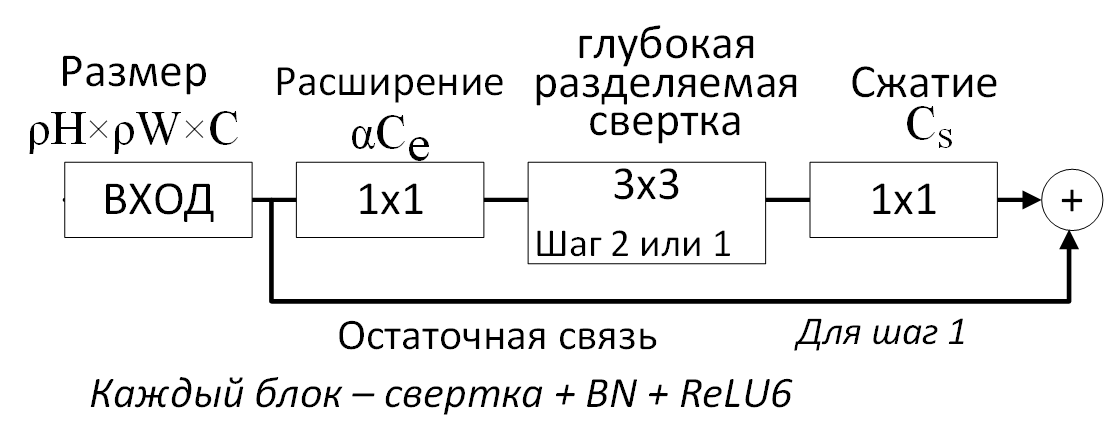
\includegraphics[width=0.99\linewidth]{./figuresch1/mobilenet_block_v1_2.png}
		\caption{Иллюстрация блока MobileNet V2}		
		\label{ch1:fig:mobilenet_block_v2}
	\end{center}
\end{figure}

%%%%%%%%%%%%%%%%%%%%%%%%%%%
\subsubsection{Попытки использования идеи "слой внимания"}
Идея "подсвечивания" для нейронной сети наиболее информативных участков входных данных (информативных с точки зрения задачи) присутствовала в сообществе исследователей нейронных сетей начиная с 1990-х \cite{itti2001computational}. В 2014 Бахданау (Bahdanau) предложил использование данной идеи в задачах машинного перевода, предложенная архитектура была названа \textbf{механизм внимания (attention)} \cite{bahdanau2014neural}. Идея механизма внимания получила широкое развитие и распространение в различных приложениях обработки естественного языка и других схожих задачах \cite{chaudhari2019attentive}. В 2016-2017 годах в работах \cite{cheng2016long, parikh2016decomposable, vaswani2017attention} была развита идея \textbf{механизма само-внимания (self-attention)} для задач обработки естественного языка. Также в работе \cite{ vaswani2017attention} были предложены т.н. \textbf{много-головое внимание (multi-head attention) и блок трансформер (transformer)}. Начиная с 2017 года идеи механизма внимания активно исследуются в приложениях к сверточным нейронным сетям в различных задачах компьютерного зрения \cite{Lilian2021Attention, yang2020overview}. Отметим, что \uline{в противовес к само-вниманию, классический механизм внимания называют \textbf{кросс-внимание (cross-attention)}}. 
Основной идеей механизма  внимания  является обучение слоя (блока)  выделять наиболее важные участки входных данных при помощи нормализации функцией softmax (\ref{ch1:eqn:softmax}) \cite{Lilian2021Attention}. В случае само-внимания слой обучается только на основе входных данных. Если речь идет о кросс-внимание то слой обучается на входных и уже предсказанных выходных данных. 
\textcolor{green}{
Иллюстрация механизма само-внимания для сверточных сетей показана на рисунке \ref{ch1:fig:conv_self_attention}}. 

%TODO: возможно надо убрать эту картинку и пояснения к ней так как такого слоя в природе нет.
\begin{figure}[!h]
	\begin{center}
		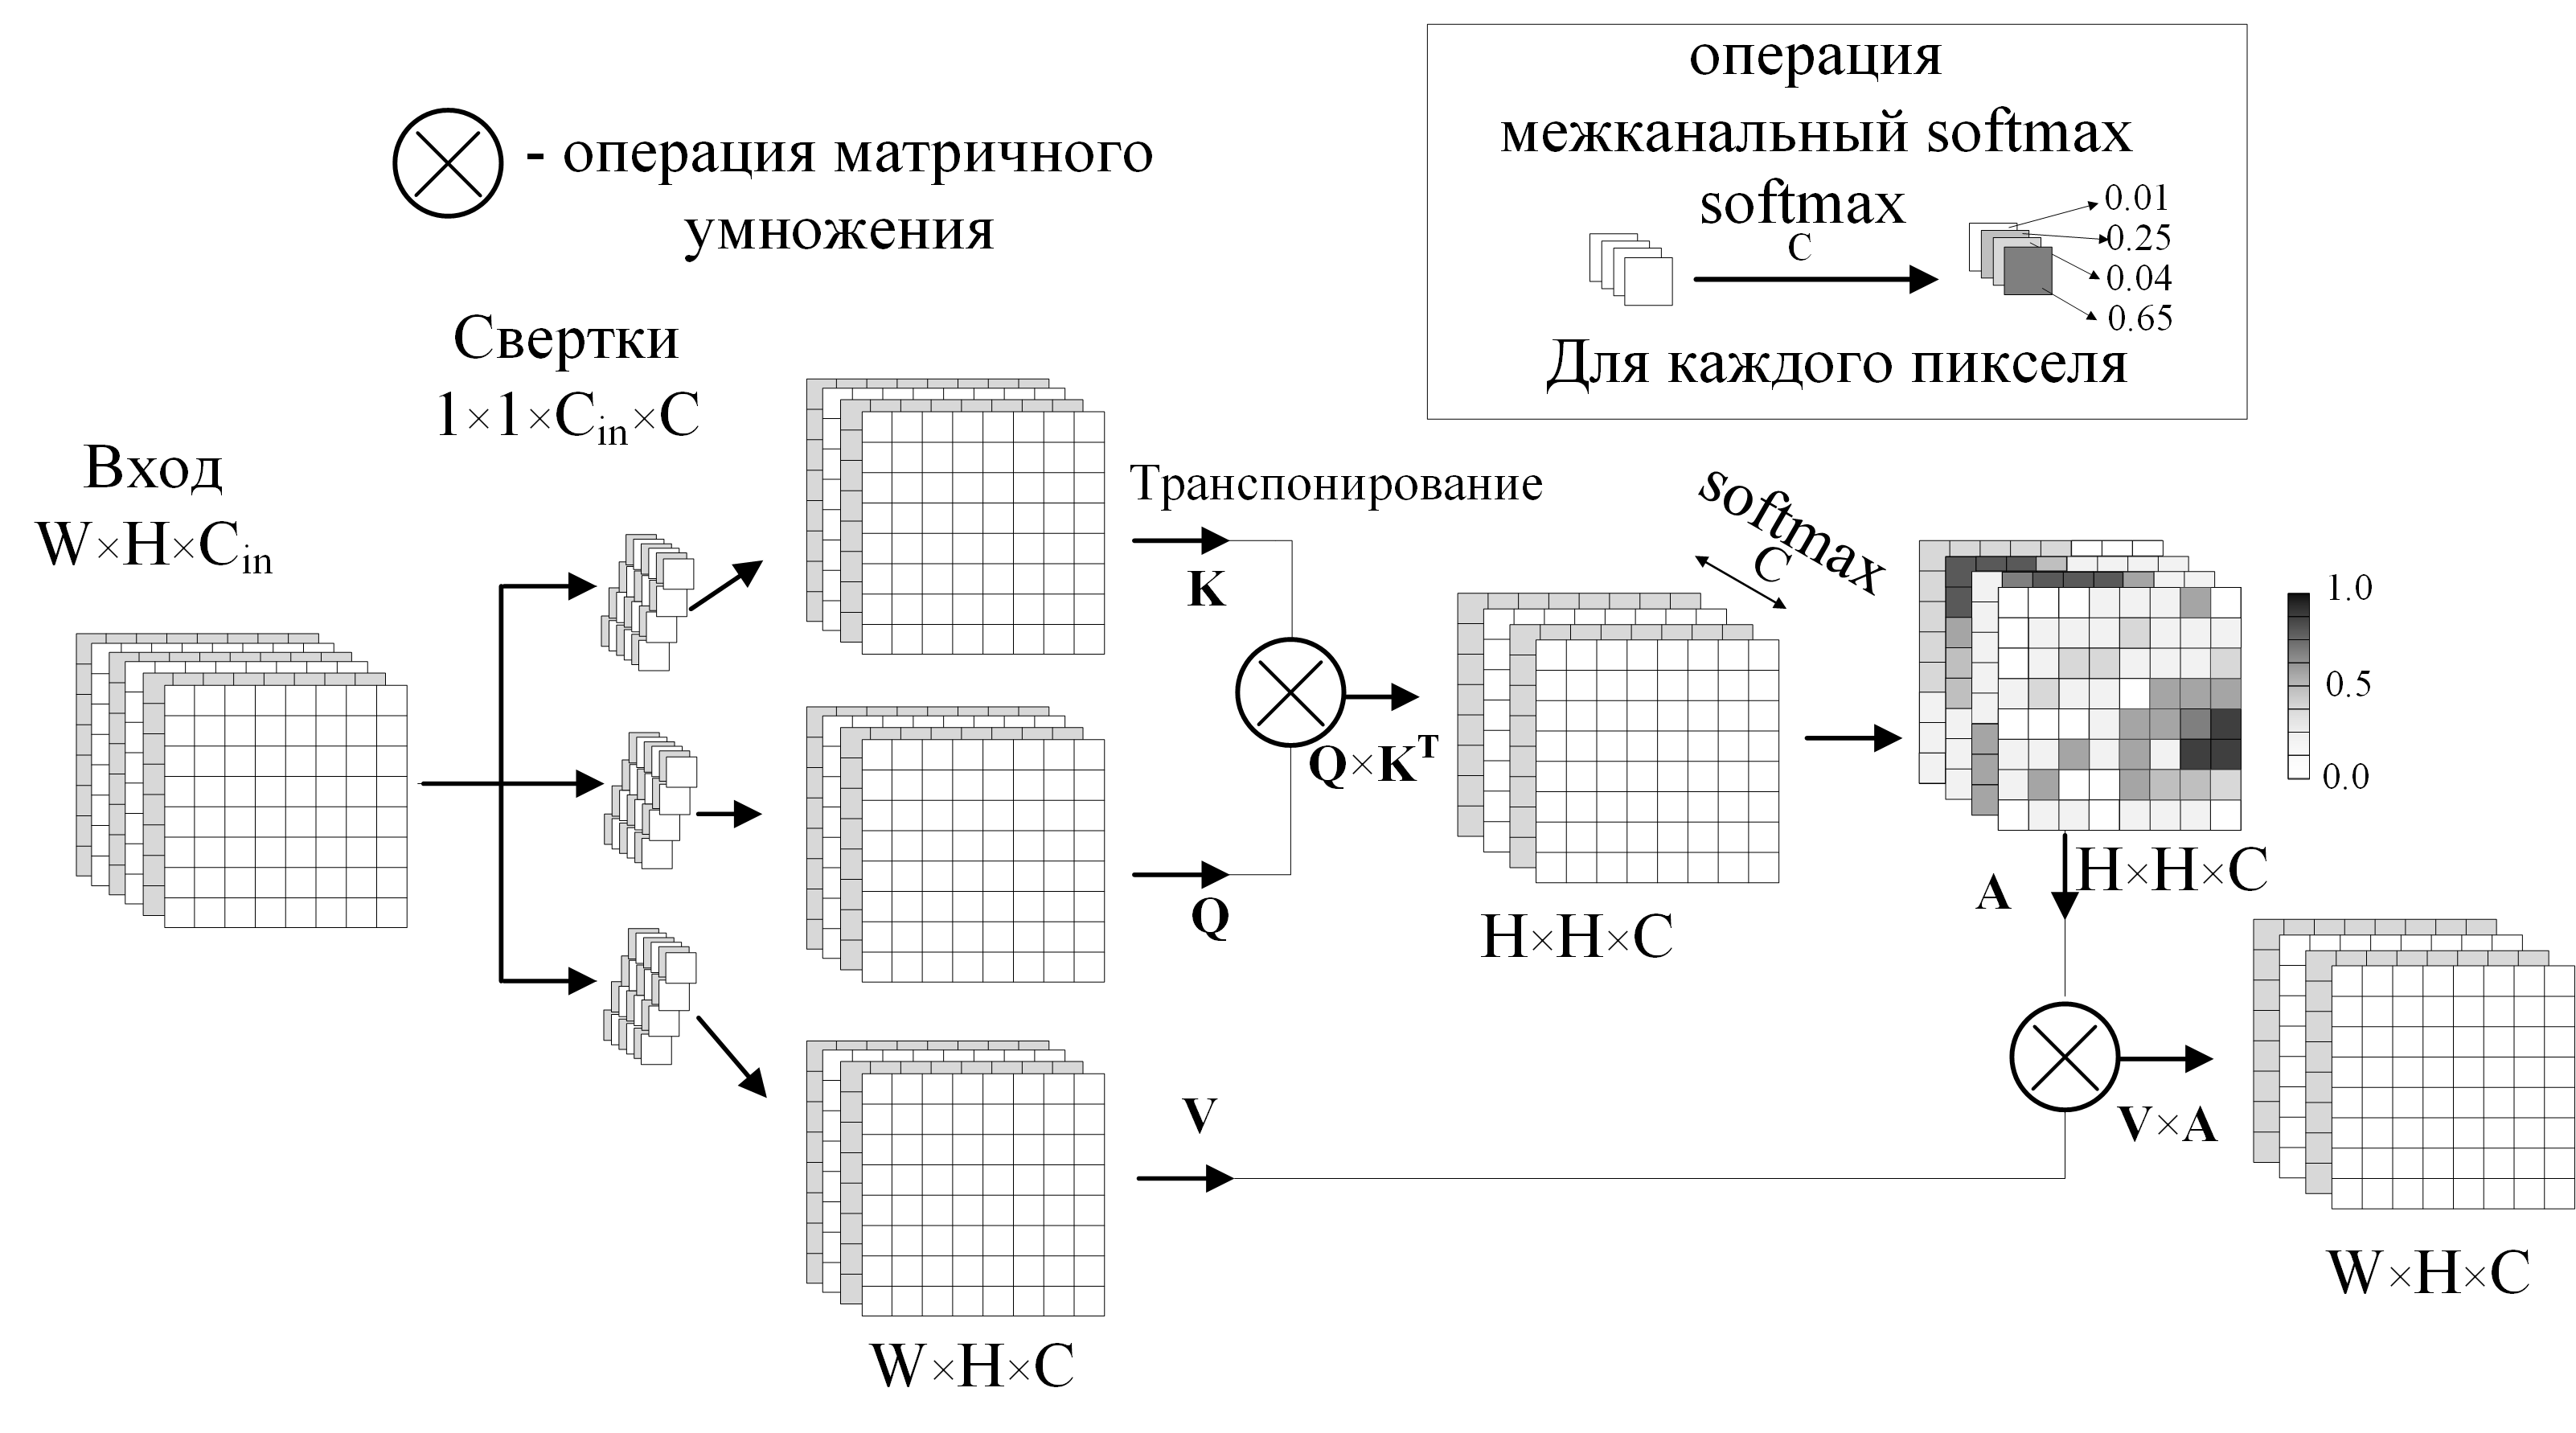
\includegraphics[width=0.99\linewidth]{./figuresch1/conv_self_att.png}
		\caption{
		\textcolor{green}
		{Иллюстрация слоя само-внимания для сверточных сетей}}	
		\label{ch1:fig:conv_self_attention}
	\end{center}
\end{figure}
\textcolor{green}{
Иллюстрация на рисунке \ref{ch1:fig:conv_self_attention} соответствует типу \textbf{меж-канальное само-внимания}, так как взвешивание функцией softmax проводится по каждой позиции пикселя, но для всех каналов.}
\textcolor{green}{
Отметим, что иллюстрация \ref{ch1:fig:conv_self_attention} это упрощенный пример авторов и носит только иллюстративный характер. Однако, архитектура такого слоя была парализована кем либо ранее. Некоторые практически используемые варианты слоя внимания будут рассмотрены в книге далее.}

В работе \cite{cordonnier2019relationship} показано, что
слой самовнимания позволяет провести перегруппировку пикселей входного слоя - то есть делает результат работ нейронной сети независимым от нерегулярных особенностей каждого экземпляра входных данных. Другими словами слой внимания дополняет одно из наиболее важных свойств сверки - инвариантность к положению объекта \textcolor{red}{(как по координатам, так и по наклону, повороту и т.д.)}. В работе \cite{cordonnier2019relationship} 2019 года авторы привели математические доказательства, что много-голове само внимание эквивалентно свертке. Однако, отметили, что вероятно, предпочтительно использовать оба типа слоев вместе. 

% В основе работы слоя, соответствующего рисунку \ref{ch1:fig:conv_self_attention} лежит идея,что при его обучении (в рамках обучения нейронной сети) набор каналов $\mathbf{A}$ (результат работы softmax) 



%%%%%%%%%%%%%%%%% SENET %%%%%%%%%%%%%%%%%%%%%
В 2017 году в работе \cite{hu2018squeeze} концепция внимания для сверточных сетей был значительно переработана. В результате 
\textcolor{red}{Jie Hu и коллективом соавторов}  был предложено \textbf{слой сжатия-возбуждения (Squeeze-and-Excitation layer, SE layer)}. Структура блока сжатия-возбуждения приведена на рисунке \ref{ch1:fig:senet}. В основе работы блока лежит идея выделения наиболее важных карт признаков (каналов) путем через автоэнкодер (верхняя часть рисунка) и затем через фикцию активации сигмоид (логистическая функция для каждого элемента). В результате такой операции формируются коэффициенты $\alpha_C$, характеризующие "важность" каждой карты признаков. Таким образом, SE Layer призван помочь нейронной сети принимать во внимание только наиболее важные (регулярные, релевантные задаче) признаки. 
Отметим, что строго говоря слой SE Layer не является блоком внимания в классическом смысле так как использует логистическую функцию активации для каждого выхода вместо единой нормализации функцией softmax. Однако, часто слой SE Layer рассматривают в качестве варианта межканального внимания. 

\begin{figure}[!h]
	\begin{center}
		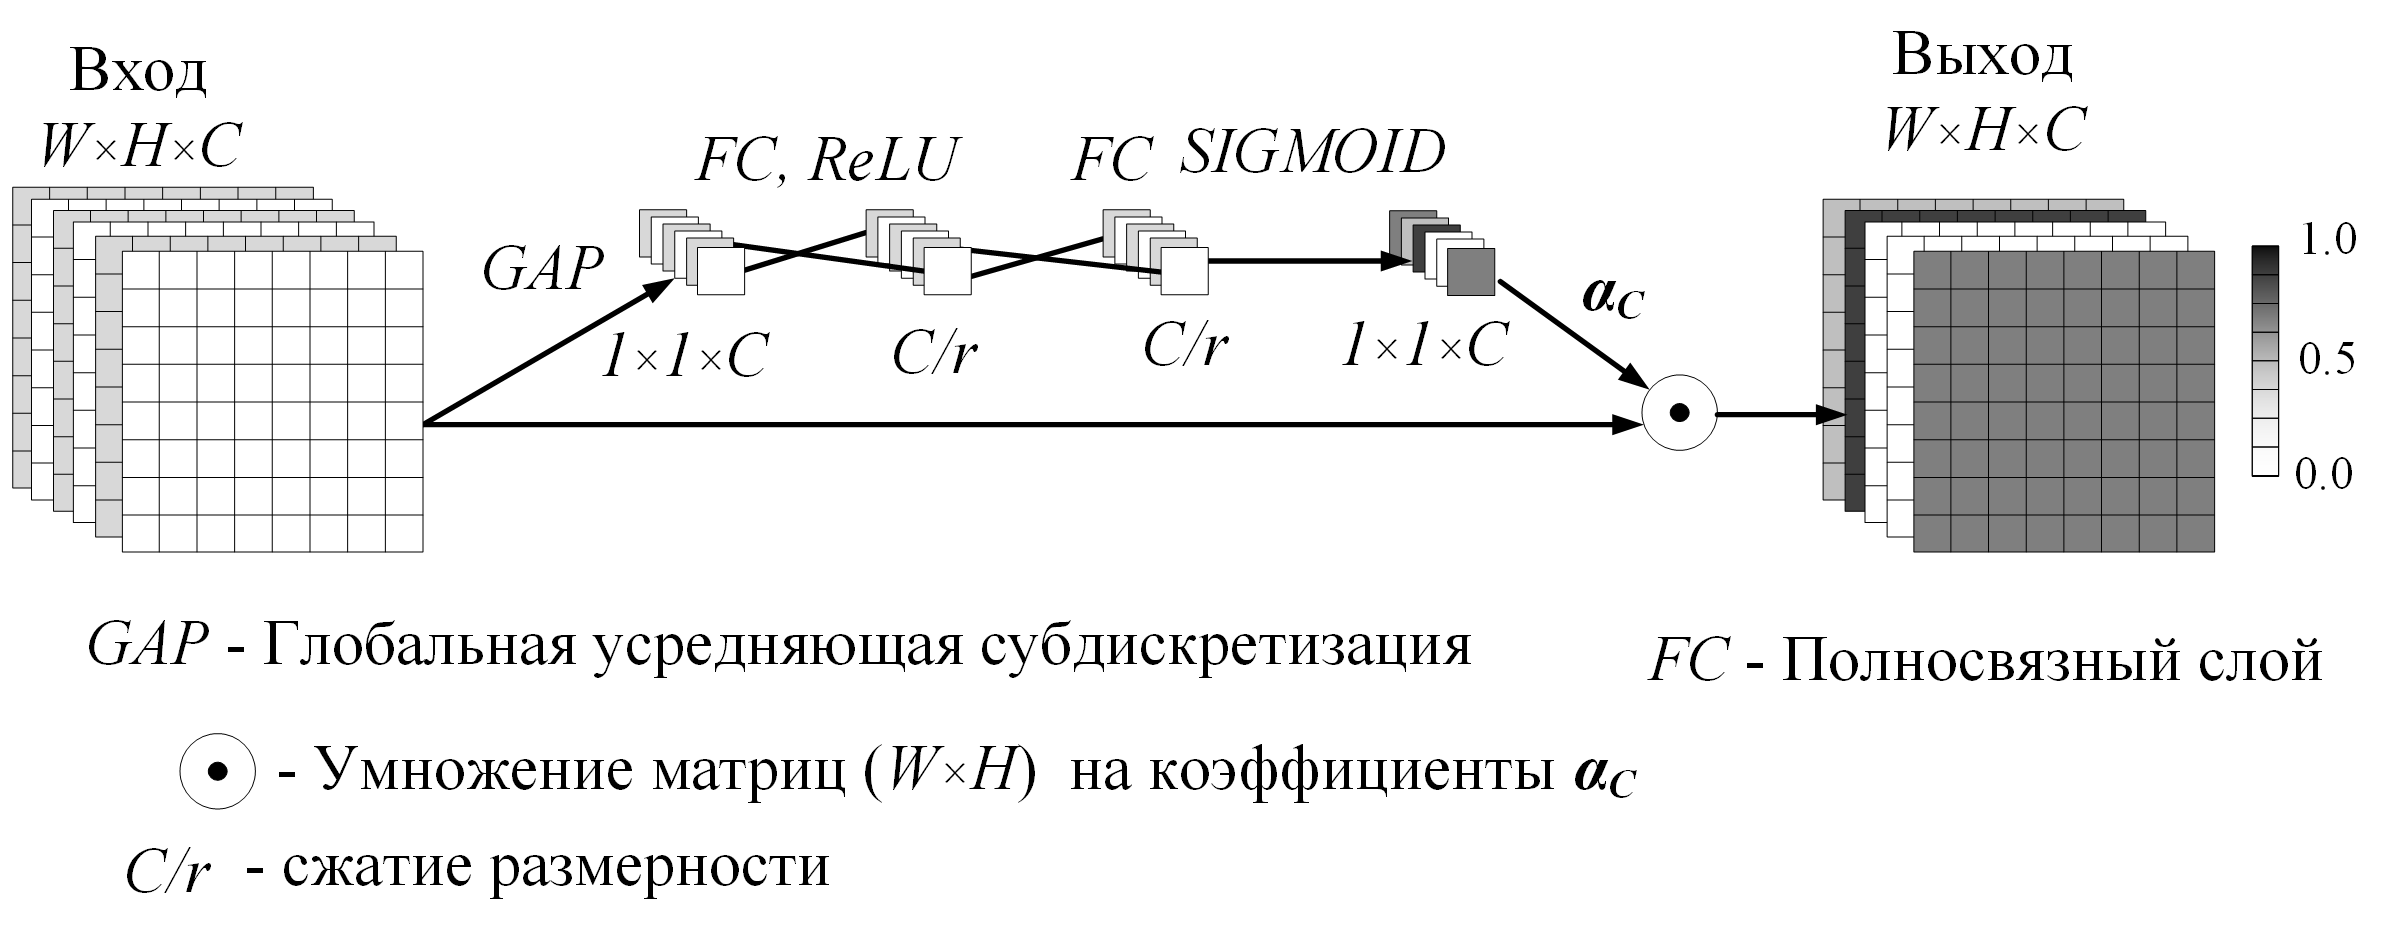
\includegraphics[width=0.99\linewidth]{./figuresch1/SELayer.png}
		\caption{Иллюстрация слоя Сжатия-возбуждения (SELayer)}	\label{ch1:fig:senet}
	\end{center}
\end{figure}

В 2017 году команда авторов работы \cite{hu2018squeeze} одержали победу в соревнования по классификации ILSVRC 2017 с ошибкой 2,25 (4,5)\% по методике top-5-accuray \cite{hu2018squeeze}. Слой SE позже был использован во многих успешных архитектурах сверточных нейронных сетей. В частности, с использование слоя SE были синтезированы блоки MobleNet V3 в 2019 году \cite{howard2019searching}.



%%%%%%%%%%%%%%%%%%%%%%%%%%%%%
\subsubsection{Автоматический поиск архитектур}
Идея автоматизации поиска архитектур нейронных сетей развивалась в сообществе исследователей с периода возникновения самой идеи глубокого обучения, по крайней мере с 2002 года \cite{Lilian2020NAS}. Однако, существенных успехов удалось достичь только в 2017 году, когда был предложен метод, известный как \textbf{Neural Architecture Search (NAS)} \cite{elsken2019neural}. Также отметим, что начиная с  2015 года проводятся соревнования по автоматическому синтезу алгоритмов машинного обучения, в том числе, но не только по автоматичесеому поиску архитектур глубокого обучения (AutoML Challenge). Также отметим, что термин AutoML - автомтаический поиск архитектур, включает, но не ограничен методами NAS \cite{hutter2019automated}.

%%%%%%%%%%%%%%%%%% NAS %%%%%%%%%%%%%%%%
По существу, \textbf{методы NAS подразумевают три составляющие.}
\begin{itemize} 
\itemsep 0.125em 
    \item \textbf{Пространство поиска (Search Space)}. Набор блоков, слоев или архитектур которые могут быть использованы. Выбор таких архитектур исходит из опыта исследователя. Отметим, что данный факт является наиболее фундаментальным ограничением методов NAS. \\
    В современных системах общая структура блоков и их максимальное число часто фиксированы, но параметры блоков (наличие пулинга, число карт признаков, размер входного массива, число остаточных связей и т.д.) могут меняться.
    \item \textbf{Стратегия поиска (Search Strategy)}. Набор правил для выбора тех или иных блоков. От выбора стратегии поиска может зависть число возможны комбинаций в пространстве поиска, как правило число комбинаций должно быть максимально ограничено. \\
    В первых работах по NAS рассматривались такие стратегии как \cite{elsken2019neural}:
    \begin{itemize} \itemsep 0.1em 
        \item генетические эволюционные алгоритмы (начало 2000-ных);
        \item методы Байесовской оптимизации (2010-е);
        \item обучение с подкреплением (2017); 
        \item рекуррентное обучение с кодированием всех вариантов в категориальные вектора (2018). 
        % \cite{zoph2018learning, zoph2018learning}.
    \end{itemize}
    \item \textbf{Оценка качества модели (Performance Estimation Strategy)}. Данный вопрос также является не тривиальным. Так как к архитектуре могут быть предъявлены совместно требования высокой точности, оптимальной производительности для конкретной конфигурации оборудования или времени работы, требования к занимаемому месту в памяти и другие требования.  \\
    Также к данному пункту относится выбор метода снижения вычислительной нагрузке при подборе архитектуры. К таким методом можно отнести следующие \cite{elsken2019neural}:
    \begin{itemize} \itemsep 0.1em 
        \item сокращение тренировочной выборки (Lower fidelity estimates); 
        \item испытания всех моделей с пониженным числом параметров (например можно снизить число карт в 2 для каждой исследуемой модели) (Lower fidelity estimates); 
        \item ранняя остановка обучения моделей с экстраполяцией результатов (Learning Curve Extrapolation); 
        \item инициализация весовых параметров новых вариантов архитектур  весовыми параметрами предыдущих вариантов (сокращает число эпох тренировки сети) (Network Morphisms);
        \item обучение единой модели, включающей все варианты и использование комбинаций ее составляющих в качестве новых предобученных моделей (One-Shot Architecture Search).  
    \end{itemize}
    Отметим, что все описанные подходы к упрощения процесса выбора архитектуры приводят к смещению конечного результата, однако могут быть использованы для ранжирования вариантов. После выбора итоговой архитектуры - она должна быть дообучена \cite{elsken2019neural}.
\end{itemize}

%%%%%%%%%%%%%%%% NASNet and PNASNet %%%%%%%%%%%%%%%%%%%%%%%
В 2018 были опубликованы результаты оказавшие наибольшее влияние на развитие NAS: Зопф Б. и соавторы (команда Google Brain) предложили архитектуру \textbf{NASNet} \cite{zoph2018learning}, а Лью Ч. в соавторстве с коллективом, включающим Зопф Б. предолжили \textbf{метод прогрессивного поиска архитектур (Progressive NAS, PNAS)}, а также архитектура \textbf{PNASNet} \cite{liu2018progressive}. 

Для синтеза NasNet использовался рекуррентный подход, предложенный Зопфом в работе \cite{zoph2016neural} и метод регуляризации путем выключения частей блоков при обучении каждого варианта архитектуры. В работе \cite{liu2018progressive} авторы  предложили стратегию последовательно усложнения структуры блоков с прореживанием пространства поиска (PNAS). Прореживание выполнялось предварительной оценкой точности для каждого из кандидатов-блоков. При этом общая структура сети фиксировалась перед проведением экспериментов. 

Архитектуры PNASNet и NASNet показали практически эквивалентные результаты для набора данных ImageNet, однако метод PNASNet потребовал в 8 раз меньше вычислительных ресурсов и при этом архитектура PNASNet требовала несколько меньшего объема памяти.
Архитектура PNASNet стала победителем на ILSVRC 2018 и достигла точности 96,2 \% (на 1,2\% выше чем вручную оптимизированные архитектуры)\cite{liu2018progressive}.

%%%%%%%%%%%%%%%%% EFFICIENT NET %%%%%%%%%%%%%%%%%%%%%%%%%%%%
В 2019-2020 годах исследователи из Google дополнили метод NAS и предложили семейства архитектур \textbf{EfficientNet V1 }(2019) \cite{tan2019efficientnet} и  \textbf{EfficientNet V2} (2020) \cite{tan2021efficientnetv2}. В основе предложенного подхода лежала идея поиска оптимальной базовой архитектуры методом PNAS (baseline)  и ее масштабирование по трем параметром - т.н. compound scaling method. Общая структура сети определялась методом PNAS, масштабированию подлежали входное разрешение, число слоев каждого блока сети (глубина) и  число карт признаков в каждом блоке (ширина). При этом масштаб изменялся с одинаковым коэффициентом для всех трех параметров \cite{tan2019efficientnet}. Семейства архитектур EfficientNet V1/V2 стали одними из основных архитектур для решения практических задач компьютерного зрения в 2020-2021 годах. Помимо официальных версий EfficientNet в литературе предложены варианты архитектур для специальных задач, например для использования в мобильных телефонах \cite{Hollemans2020NewMB}.


%%%%%%%%%%%%%%%%%%%%%%%%%%%%%%%%%%%%%%%%%%%%%
\subsubsection{Архитектуры типа трансформер в задачах компьютерного зрения}
Как уже было сказано ранее в 2017 году различными исследователями было предложено использование идеи слоев внимания в задачах компьютерного зрения. Также в 2017 году А. Васвани  был предложен блок, названный трансформер (transformer) для задач обработки естественного языка \cite{ vaswani2017attention}. В составе данного блока использовались только слои внимания и полносвязные слои. В 2018 году было предложено использовать блока трансформер в задачах генерации изображений и обработки видео. В 2020 году были предложены первые успешные архитектуры для задачи классификации изображений \cite{han2020survey}. Многими авторами предлагалось замена части слоев сверточных сетей на блоки трансформеры (полносвязные блоки с вниманием (такие же как Васвани)) \cite{lin2021survey}. В 2020 году была предложена архитектура ViT, в которой авторы использовали только блоки трансформеры и смогли достичь точности на наборе ImageNet сопоставимой со сверточными сетями. По существу, архитектура ViT являлась переосмыслением архитектуры BERT для обработки естественных языков (2018 г. \cite{devlin2018bert}). Иллюстрация архитектуры ViT показана на рисунке \ref{ch1:fig:transformer_vit}. 

\begin{figure}[!h]
	\begin{center}
		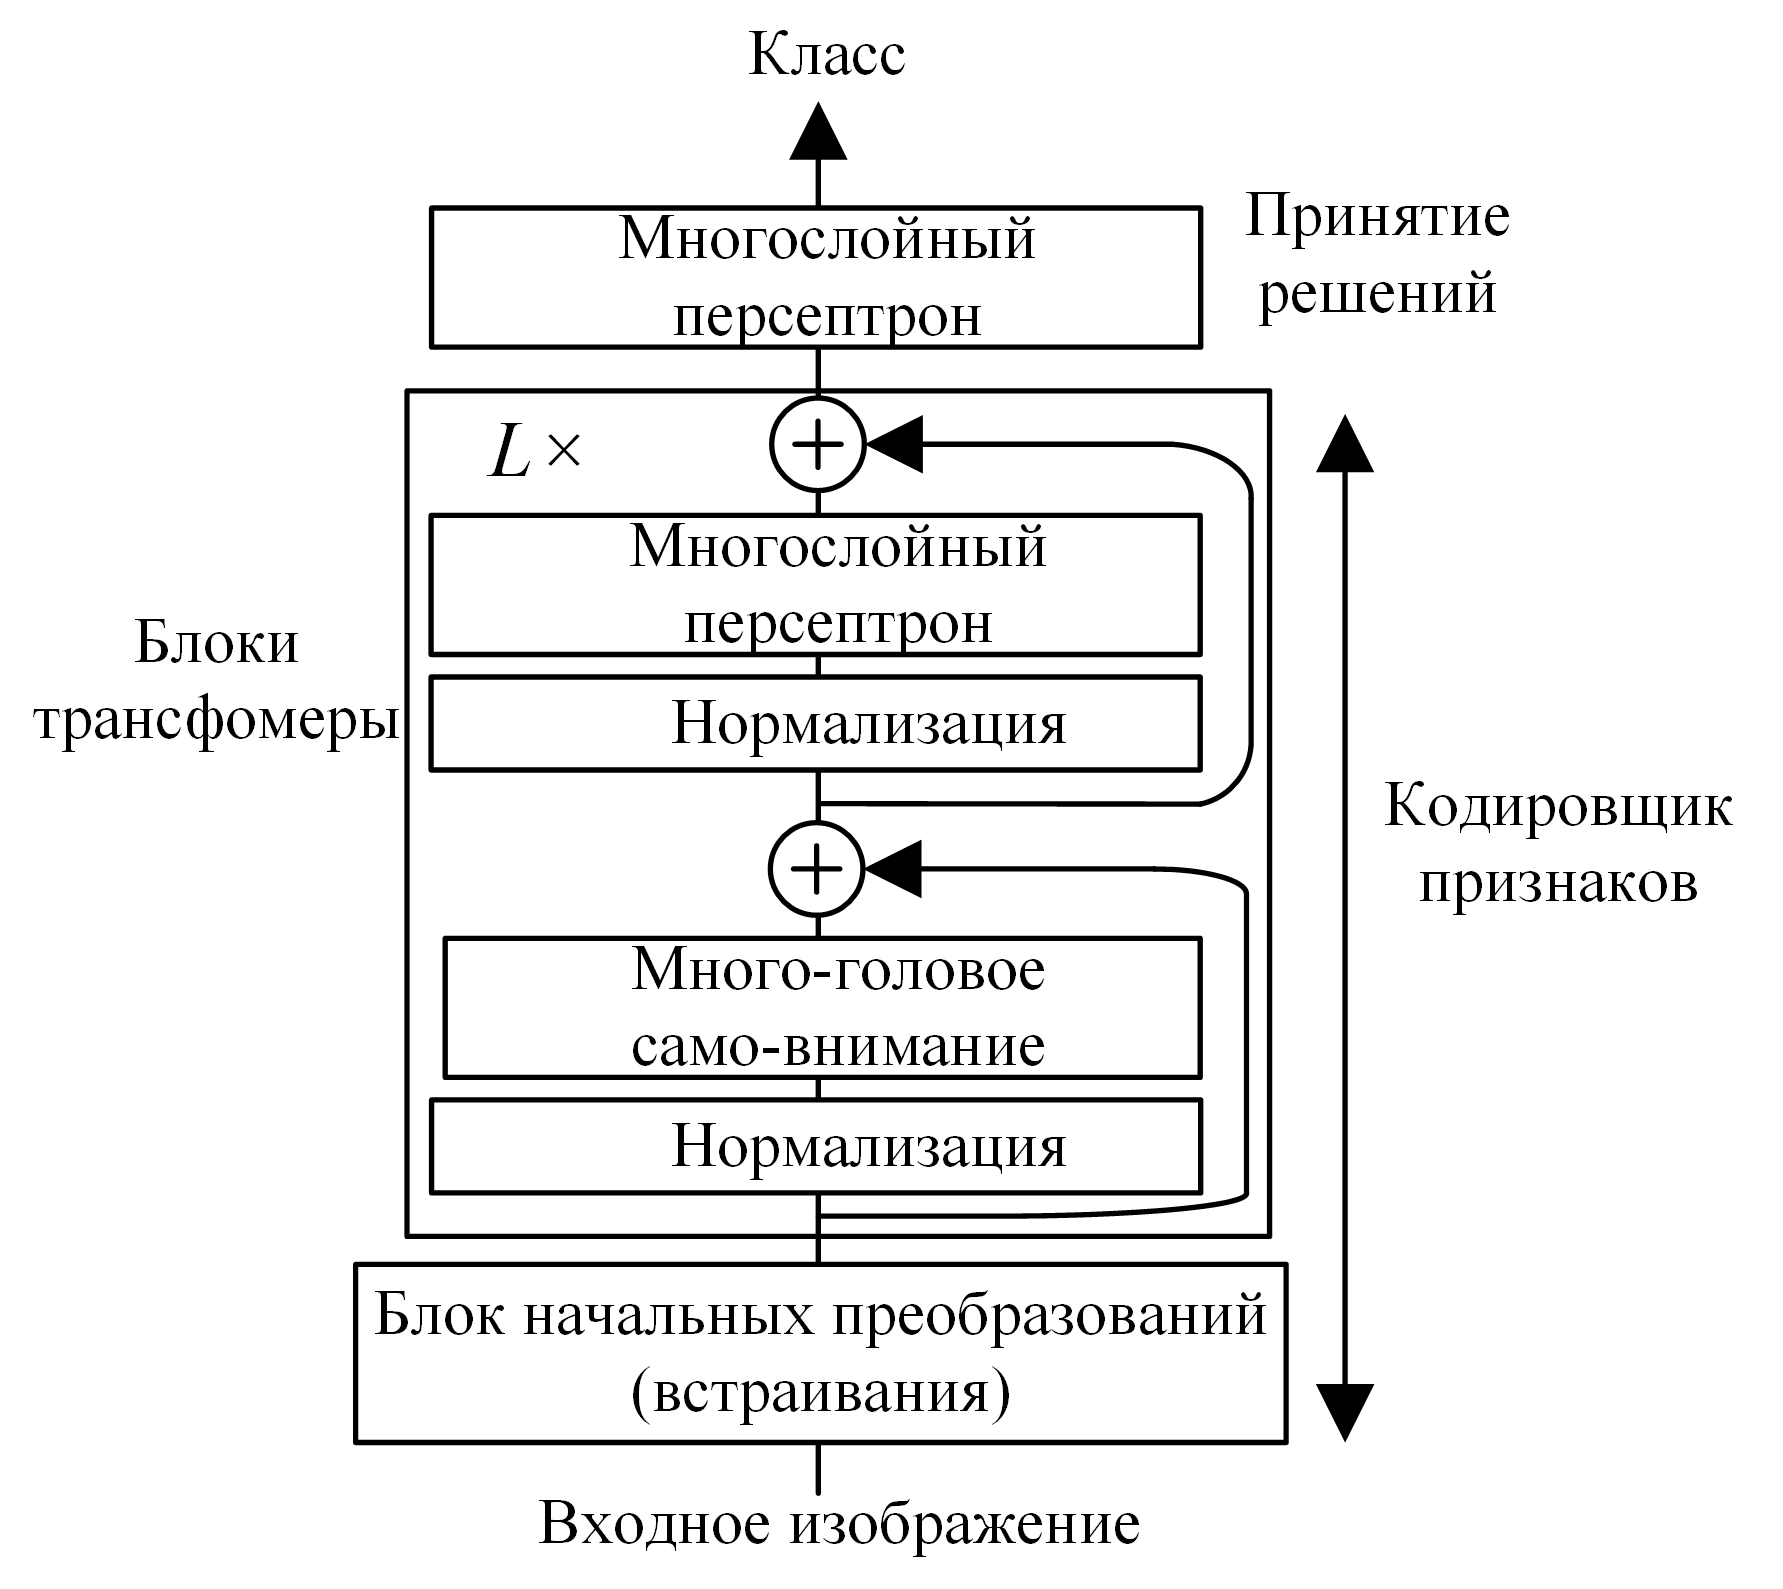
\includegraphics[width=0.7\linewidth]{./figuresch1/transformer_vit.png}
		\caption{Иллюстрация архитектуры ViT}	
		\label{ch1:fig:transformer_vit}
	\end{center}
\end{figure}

Архитектура ViT состоит из блока начальных преобразований; набора слоев трансформеров и блок принятия решений на основе многослойного персептрона. Блоки трансформеры и блок начальных преобразований образуют кодировщик признаков. Каждый блок трансформер состоит из слоев нормализации, слоя много-голового само-внимания и многоголового персептрона. Таким обзорам архитектура ViT не имеет сверточных слоев. 
\textcolor{red}{
Более подробная иллюстрация ViT приведена на рисунке \ref{ch1:fig:transformer_vit_v2}. Иллюстрация показана для архитектуры ViT-L c 16 каналами многоголового само-внимания.
\begin{figure}[!h]
	\begin{center}
		\includegraphics[width=0.99\linewidth]{./figuresch1/vit_v3.png}
		\caption{Подробная иллюстрация архитектуры ViT-L}	
		\label{ch1:fig:transformer_vit_v2}
	\end{center}
\end{figure}
}
Архитектура ViT стала первой доказавшей, что решение задач компьютерного зрения возможно по средствам полносвязных нейронных сетей. Данная модель показала точность 88,5\% по методу top-1 на наборе данных ImageNet. Однако, для достижения высокой точности модель ViT была предобучена на наборе данных JFT-300M (набор с 300 млн. изображений \cite{sun2017revisiting}) \cite{dosovitskiy2020image}. Отмечается, что в случае предобучения на небольших наборах данных (менее 14 млн изображений) точность модели ViT значительно снижается (примерно до 75\%). Также число параметров ViT в 10 раз выше чем для сверточной сети (~ 600 тыс. параметров). Архитектура ViT стала одним из основных этапов в принятии трансформеров сообществом исследователей систем компьютерного зрения \cite{khan2021transformers}. Позже в работе \cite{touvron2021training} была предложена архитектура DeiT, в которой число параметров было снижена до ~ 80 тыс. и при этом модель показала точность 83,5\% по методу top-1 на наборе данных ImageNet с использованием только данных ImageNet (без предобучения на JFT-300M). В конце июня 2021 года была также представлена архитектура Vision Outlooker (VOLO) показавшая точность 85,5\% в условиях аналогичных  DeiT, однако имеющая больше параметров \cite{yuan2021volo}. Также июне была представлена модель ViT-G, показавшая точность 90,5\% по методу top-1 на наборе данных ImageNet и имеющая порядка 2-х миллиардов параметров \cite{zhai2021scaling}.

Главными достоинствами архитектур трансформеров являются следующие \cite{khan2021transformers, han2020survey}.
\begin{itemize} \itemsep 0.2em 
    \item Возможность построения сложных зависимостей между признаками локальными участков изображения независимо от их взаимного расположения. 
    \item Трансформеры позволят обучать модели с значительно увеличенным числом параметров. Что также дает преимущества при предобучении на больших наборах данных, таких как JFT-300M. В предыдущие эпохи (до 2015 гг) данное обстоятельство скорее было недостатком. В настоящее время в силу развития вычислительной техники и возможностей сети Интернет имеется возможность сравнительно быстрой работы с большими объемами данных. При этом путь повышения точности и обобщающей способности за счет предобучения является предпочтительным.
    \item Возможность для некоторых архитектур предобучения на не размеченных данных. Ряд архитектур трансформеров имеют возможность предобучаться подобно жадному предобучению о котором говорилось выше. Такая возможность особенно важна в силу сказанного в предыдущем пункте. Также отмечается \cite{gidaris2018unsupervised, jing2020self}, что предобучения баз разметки потенциально способствует повышению выразительной силы (сложности признаков) и обобщающей способности нейронной сети. Метод предобучения на не размеченных данных принято называть \textbf{self-supervised learning (самообучение).} 
\end{itemize}

%%%%%%%%%%%%%%%%%%%%%%%%%%%%%%%%%%
\newpage
\subsection{Обзор других задач компьютерного зрения}

В данном разделе преимущественно говорилось о задаче классификации изображений. Данная задача в определенном смысле была первой задачей компьютерного зрения, в которой появилась крайняя необходимость в использовании методов машинного обучения и в которой глубокие нейронные сети показали преимущества перед остальными методами. Как уже сообщалось в книге в первую очередь это было связано с автоматизацией выделения признаков изображений (в отличии от остальных методов, где требовалась формализация признаков и их описание "вручную"). Однако, задачи компьютерного зрения не ограничиваются задачей классификации изображений. В данном \textcolor{red}{разделе} кратко будут названы и описаны другие типичные задачи компьютерного зрения. Отметим, что архитектуры нейронных сетей для задачи классификации, которые описывалась ранее являются основой для решения других задач компьютерного зрения. Правильней даже будет сказать так, что кодировщики признаков (см. энкодер  рисунок~\ref{ch1:fig:LeNet5}), являющиеся основной частью архитектур для классификации, используются при решении других задач компьютерного зрения.

Среди основных задач компьютерного зрения могут быть выделены следующие задачи, которые как правило справедливы как для отдельных изображений, так и для видео-сцен 
\cite{srinivas2016taxonomy}.
\begin{enumerate} \itemsep 0.05em 
    \item Классификация (рассмотрена выше).
    \item Обнаружение и локализации объектов (Object Detection, 
    Object Localization). 
    \item Сегментации классов объектов и сцен (Semantic Segmentation).
    \item Объектная сегментация (Instance Segmentation).
    \item Сегментации объектов и сцен (Panoptic Segmentation).
    \item Поиск и выделения ключевых точек (Key-Point Detection).
    \item Генерации изображений (Image Generation).
    \item повышение качества изображений и видео-сцен (Super-Resolution).
\end{enumerate}
\textcolor{red}{
Среди описанных выше задач в книге будут рассмотрены 1-3 и 7, а также сопутствующие им задачи.}

%%%%%%%%%%%%%%%%%%%%%%%%%%%
\subsubsection{Кратко о задаче семантической сегментации}
Задача семантической сегментации известна в приложениях компьютерного зрения достаточно давно \cite{sultana2020evolution, thoma2016survey}.  Однако, первые успешные попытки ее решения при помощи нейронных сетей были опубликованы в 2012 году в работе С.Farabet и соавторов \cite{farabet2012learning}. В частности, в данной работе был предложен пиксельной классификации - то есть присвоение класса каждому пикселю входного изображения. То есть результатом работы нейронной сети должен стать набор карт признаков - по одной для каждого класса. При этом каждая карта признаков должна выделить всю площадь (или контур) объектов данного класса. Для повышения надежности сегментации объектов разных масштабов в работе предлагалось использовать несколько сверточных энкодеров признаков и затем объединить полученные карты. Однако, архитектура, предложенная в \cite{farabet2012learning} не получила широкого распространения. Таким образом, в рамках этой и последующих архитектур глубокого обучения нейронных сетей задача семантической классификации может быть рассмотрена как расширение идеи классификации, но классификации по каждому пикселю выходной карты признаков.

В 2014 году в работе J. Long и соавторов \cite{long2015fully} была предложена \textbf{полностью сверточная архитектура (fully convolutional network (FCN))} сети семантической сегментации. В данной архитектуре авторы модифицировали архитектуру AlexNet (см. рисунок~\ref{ch1:fig:alexnet}). Было предложено  заменить последние слои (головную часть, см. рисунок~\ref{ch1:fig:LeNet5}) на сверточные слои и после них поставить слой увеличения размерности при помощи передескретизации (upsampling, unpooling) \textbf{методом билинейной интерполяции (bilinear interpolation)}. Суть данного метода будут рассмотрена позже \cite{long2015fully}. В 2015 году в работе \cite{noh2015learning} была предложена архитектура архитектура сверточной нейронной сети с использованием слоев т.н. обратная (транспонированная) свертка (deconvolution, transposed convolution) и повышающей передискретизации. Архитектуру было предложено назвать \textbf{DeconvNet}. Иллюстрация архитектуры DeconvNet приведена на рисунке \ref{ch1:fig:DeconvNet}. В данной архитектуре для выполнения операции unpooling выполнялась путем сохранения индексов пискселей, прошедших процедуру прямую дискретизации в соответствующих слоях.  Позже в 2015 году архитектура была оптимизирована и опубликована в работе \cite{badrinarayanan2015segnet} под названием \textbf{SegNet}. По существу, архитектура DeconvNet состоит из двух частей: кодировщик признаков (энкодер) и декодировщик признаков (декодер), а также слоя пописксельной классификации. Цель использования энкодера заключается в выделение релевантных признаков во входных данных. Цель использования декодера заключается в восстановлении из выделенных признаков т.н. маски целевого класса (силуэт или контур соответствующего объекта или сцены). Число выходных карт признаков (выходных каналов) сети должно соответствовать числу классов на которые должно быть поделено (сегментировано) изображение. Решение о том, к кому классу принимается путем использования операции softmax между всеми каналами по каждому пикселю. Таким образом, каждый выходной канал содержит силуэт соответствующий одному целевому классу.

     \begin{figure}[!h]
    	\begin{center}
    		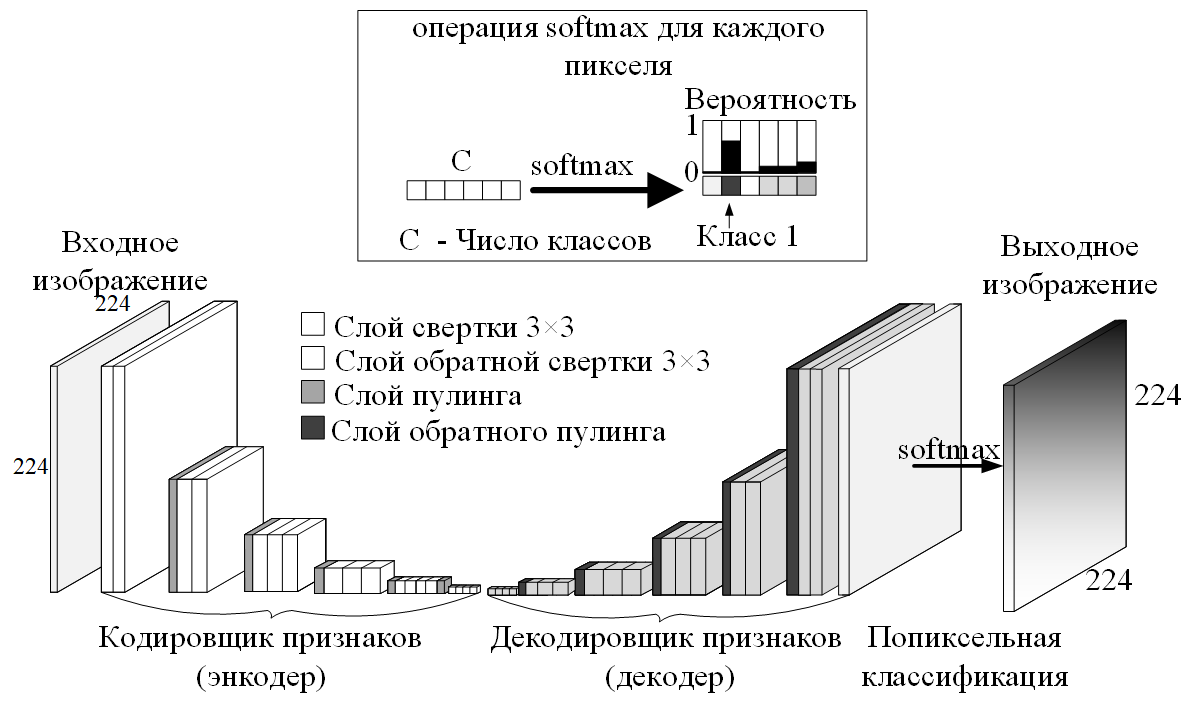
\includegraphics[width=0.99\linewidth]{./figuresch1/DeconvNet_v3.png}
    		\caption{Иллюстрация  архитектуры  DeconvNet}	
    		\label{ch1:fig:DeconvNet}
    	\end{center}
    \end{figure}

В 2015 году  O. Роненбергом и соавторами была предложена архитектура U-Net \cite{ronneberger2015u}.  Особенностью данной архитектуры было использование в декодирующей части архитектуры совмещенных (конкатенация) карт признаков энкодера и декодера. Такой подход позволил существенно увеличить точность особенно в случае малоразмерных деталей изображения. Изначально архитектура U-Net была предложена для решения медицинских задач \cite{punn2021modality}. В настоящее время архитектура является одной из наиболее популярных среди любых задач, сводящихся к семантической сегментации (по данным портала paperswithcode.com) \cite{paperswithcodeSemanticSegmentation}. Однако, U-Net и не является наиболее точной архитектурой, например для классического набора данных PASCAL VOC 2012 \cite{pascalVOC} по данным портала paperswithcode.com \cite{paperswithcodePASCALVOCSematic}. Иллюстрация архитектуры U-Net приведена на рисунке \ref{ch1:fig:UNet}. 

     \begin{figure}[!h]
    	\begin{center}
    		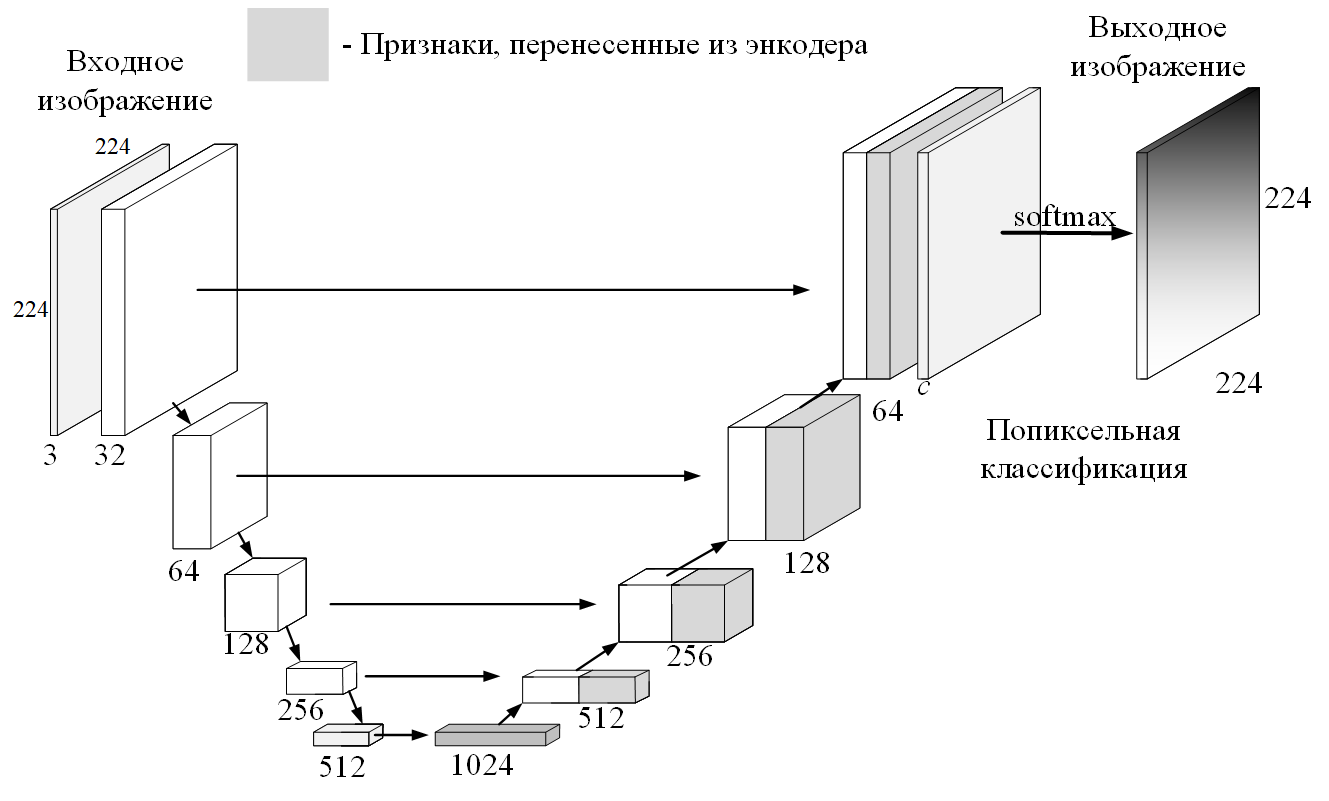
\includegraphics[width=0.89\linewidth]{./figuresch1/UNet.png}
    		\caption{Иллюстрация  архитектуры  U-Net}	
    		\label{ch1:fig:UNet}
    	\end{center}
    \end{figure}
    
После 2015 года различными авторами были предложены большое количество архитектур на основе U-Net и DeconvNet \cite{taghanaki2021deep}.
В том числе, наиболее успешные архитектуры, которые, однако переосмыслены с использованеием расширенных понятий свертки (речь о котором пойдет в свое время) и с использованием метода NAS. 
Отметим, что, в описанных архитектурах семантической сегментации предполагается подход обучения с учителем. Однако, в литературе также обсуждаются архитектуры семантической сегментации с т.н. слабым обучением (weak supervised) - то есть с использованием только классов объектов на изображении или частичной разметки и меток классов \cite{zhang2020survey}.   

%%%%%%%%%%%%%%%%%%%%%%%%%%%
\subsubsection{Кратко о задачах Object Detection и Instance Segmentaiton}
Идеи использования нейронных сетей для обнаружения и локализации объектов возникают по крайней мере начиная с 1990-х годов \cite{vaillant1994original, rowley1998neural}. Одной из первых удачных попыток создания полностью сверточной нейронной сети для обнаружения объектов можно считать архитектуру Overfeat (2013 год) \cite{sermanet2013overfeat}. 
%https://towardsdatascience.com/overfeat-review-1312-6229-4fd925f3739f - overfeat
%https://lilianweng.github.io/lil-log/2017/12/15/object-recognition-for-dummies-part-2.html
\uline{Наиболее важной работой в области обнаружения и локализации объектов является работа 2014 года \cite{girshick2014rich} Girshick R. и соавторов из университета Беркли.}\uline{Авторы \cite{girshick2014rich} предложили архитектуру \textbf{регионная сверточная нейронная сеть (Regions with CNN features, R-CNN)}}. Данная архитектура объединила в себе наиболее продуктивные на тот момент практики в области обнаружения и локализации объектов.

Иллюстрация принципа работы архитектуры R-CNN приведена на рисунке 	\ref{ch1:fig:R_CNN}. Сеть R-CNN осуществляет предсказание области нахождения объекта и его класса в два этапа - поэтому такой подход называется \textbf{много-этапное обнаружение (multi-stage object detection)} \cite{girshick2014rich}. 

    \begin{figure}[!h]
    	\begin{center}
    		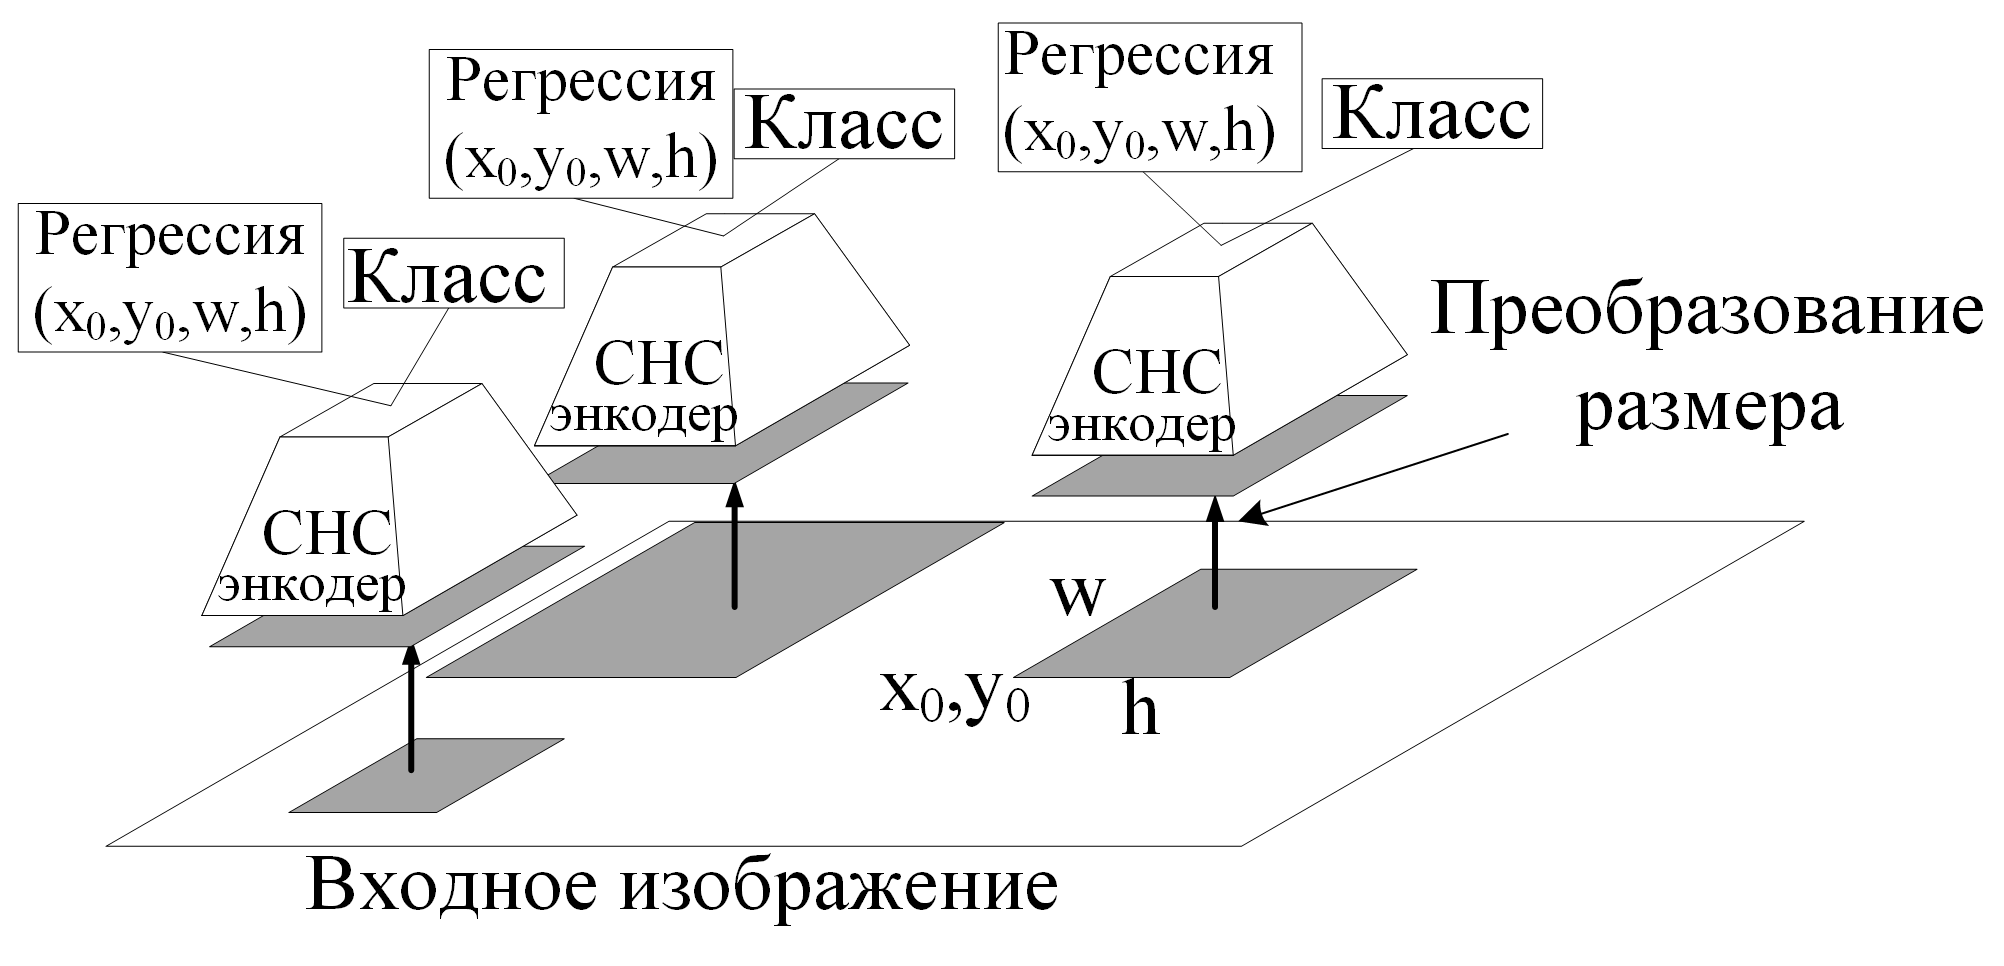
\includegraphics[width=0.99\linewidth]{./figuresch1/R_CNN.png}
    		\caption{Иллюстрация  принципа работы  архитектуры R-CNN}	
    		\label{ch1:fig:R_CNN}
    	\end{center}
    \end{figure}

Архитектура R-CNN работает следующим образом \cite{girshick2014rich}.
\begin{itemize} \itemsep 0.0em
    \item 0 Этап - подготовка перед началом обучения.
    \begin{itemize}\itemsep 0.0em
        \item Производится выбор 2000 регионов изображения, в которых предположительно есть объекты (\textbf{Regeons of Interest, ROI}). Авторы отмечают, что поиск может быть выполнен любым алгоритмом. 
        \item  В оригинальной статье выбор регионов проводится методом селективный поиск (selective search). Это метод  в котором выделяются контуры на изображении и проводится объектов в рамках контуров путем оценки схожести соответствующих участков изображения \cite{uijlings2013selective}.
        \item \qquad Все выделенные регионы могут иметь разный размер. Выделенные регионы могут как содержать целевой объект, так и нет.
        \item Отметим, что 
        \uline{данный этап используется только как подготовка изображения к обработке нейронной сетью, то есть этап не включен в работу нейронной сети}.
    \end{itemize}
    \item  1 Этап - Автоматическое выделение признаков.
    \begin{itemize}\itemsep 0.0em
        \item Производится сжатие всех выделенных регионов до одного размера. 
        \item Производится автоматическое выделение признаков (вектор 4096 значений). Выделение признаков производится при помощи сверточной нейронной сети AlexNet, в которой удален слой классификации - то есть при помощи кодировщика (энкодера) признаков AlexNet (см. \ref{ch1:fig:alexnet}).
    \end{itemize}
    \item  2 Этап - классификация регионов.
    \begin{itemize}\itemsep 0.0em
        \item Много-меточная (multilabel) классификация всех регионов ROI. Авторы используют для этого метод опорных векторов (SVM) отдельно для каждого класса.
        \item Удаление лишних регионов методом \textbf{не максимальное сжатие (non-maximum supression, NMS)}.
        В наиболее простом виде метод NMS заключается в следующем: 
        \begin{itemize}
        \item для каждого класса производится поиск регионов с относительной площадью пересечения (\textbf{Intersectino over Uninon, IoU}) больше заданного порога; 
        \item среди найденных регионов остается регион с наибольшей вероятность классификации (с наибольшим результатом выхода классифицирующего слоя).
        \end{itemize}
    \end{itemize}
    \item 3 Этап - предсказание области новых регионов.
    \begin{itemize}\itemsep 0.0em
    \item область нахождения каждого объекта описывается \textbf{граничным прямоугольником (bounding box)}. Такой прямоугольник задается начальными координатами $x_0, y_0$, а также шириной и длинной ($w, h$).
    \item Для предсказания новых значений  $x_0, y_0, w, h$ для каждого ROI используется регрессионный оконечный слой с 4 выходами (по одному на каждый параметр). Как к и в случае классификации слой используется поверх вектора признаков, полученного на 1-м этапе.
    \end{itemize}
    \item В режиме тренировки нейронной сети для новых значений  $x_0, y_0, w, h$ производится следующая эпоха обучение нейронной сети (начиная с этапа 1).
    \item В режиме работы нейронной сети выходами являются объекты, прошедшие процедуру NMS, для которых присвоена метка класса и координаты bounding box: $x_0, y_0, w, h$.
\end{itemize}
Отметим, что в оригинальной статье \cite{girshick2014rich} кодировщик признаков был предобучен на наборе данных ImageNet. Сеть была протестирована на наборе данных для решения задач обнаружения объектов PASCAL VOC \cite{pascalVOC}. Также отметим, что в литературе рассматриваются и исследуются различные модификации таких операций, как NMS и других, использованных в головной части R-CNN \cite{zou2019object}. 

В 2015 Girshick R. и соавторы предложили усовершенствованный вариант RCNN, называемый \textbf{Fast-RCNN} \cite{girshick2015fast}. Главным отличием новой архитектуры стал перенос операции от предварительного селективного поиска с этапа подготовки изображения на этап после энкодера. Таким образом авторам удалось увеличить скорость работы сети в порядка 10 раз. Отметим, что, по существу, селективный поиск по карте признаков представляет собой определенный пулинг называемые ROI Pooling, идея такого пулинга была вдохновлена работай Кайменга Хе посвященной сети с пространственным пирамидальным пулингом (SppNet) \cite{he2015spatial}. Позже в 2015 году в работе \cite{ren2015faster} коллективом авторов, включающим как Кайменга Хе, так и Girshick R. было предложено заменить селективный поиск на небольшую дополнительную нейронную сеть прогнозирующую регионы ROI (Regeon Proporsal Network, RPN). Подход был назвал \textbf{Faster-R-CNN}. В 2017 году Кайменгом Хе и соавторами, в том числе  Girshick R. было предложено улучшение архитектуры  Faster-R-CNN, в том числе дополнительно к операциям классификации и определения координат объекта было предложено добавить небольшую сверточную сеть семантической сегментации результатов ROI. Архитектуру было предложено назвать \textbf{Mask-R-CNN} \cite{he2017mask}. Архитектура  Mask-R-CNN позволяет повысить точность решения задачи определения и локализации объектов, а также позволяет решить задачу объектной сегментации (Instance segmentaion).  
%TODO: возможно это не надо
% \textcolor{red}{
% Отметим, что в Faster-R-CNN  для предсказания RoI по карте признаков на выходе RPN движется окно, выходы которого предсказывают для каждого центра окна несколько прямоугольников, различающихся масштабом и соотношением сторон, центры таких прямоугольников называются анхоры  (якоря, anchor). Из всех анхорных прямоугольников остается один с наибольшей достоверностью нахождения объекта - он считается boundig box.}

Архитектуры Faster-R-CNN и Mask-R-CNN одни из наиболее популярных для решения задач обнаружения и локализации объектов \cite{zou2019object}. А также Mask-R-CNN остается одной из наиболее популярных архитектур для решения задачи объектной сегментации \cite{hafiz2020survey}. Однако, данные сети не являются наиболее точными для классических тестовых наборов данных, таких как COCO \cite{lin2014microsoft} по данным ресурса paperwithcode.com \cite{paperswithcodeCOCOdet,paperswithcodeCOCOinst} . 


% https://towardsdatascience.com/fast-r-cnn-for-object-detection-a-technical-summary-a0ff94faa022
% Another paper published in 2015, SPP-Nets or “Spatial Pyramid Pooling Networks”[3] solved one part of the problem. Its main contribution was a) the use of multi-scale pooling of image features to improve the network performance for classification and detection and also b) the use of arbitrary sized input images to train CNN’s despite the use of fully connected (FC) layers. In its detection pipeline, it introduced an important concept— extracting a single feature map from the entire image only once, and pooling the features of arbitrary sized “region proposals” for that image, from this single feature map. This allowed their network to run orders of magnitude faster than R-CNN. Instead of running a CNN on 2000 region proposals from an image individually like R-CNN, they have only one forward pass from which they can pool the features of all 2000 candidate proposals.

В 2016 году в работе \cite{redmon2016you} Редмондом Й. и соавторами была предложена "быстрая" - одно-этапная архитектура для решения задач обнаружения объектов. Архитектуру было предложено называть \textbf{YOLO} (you look only onece). Архитектура YOLO состоит из энкодера признаков (модифицированного Inception GoogLeNet см. рисунок ~\ref{ch1:fig:inception_layer} \cite{szegedy2015going} ) и набора выходных слоев. Последний выходной слой содержит $K$ каналов по $S\times S$ ячеек. По задумке авторов, каждая из $N = S\times S$ ячеек должна соответствовать определенной части входного изображения. Число выходных каналов определяется как $B\times5+C$, где $B$ - число возможных боксов для каждой ячейки; $C$ - число классов; цифра 5 - это значения предсказанных координат и размеров бокса ($x,y,w,h$) и уверенности в том, что в боксе есть объект. В оригинальной работе $S=7, B=2, C=20$. Таким образом YOLO может предсказать до  $N = S\times S$ объектов, принадлежащих $C$ классам, если каждый объект достаточно мал, чтобы быть спровоцированным на одну ячейку. 
\textcolor{red}{
Если один объект попадает на несколько ячеек, то для определения его координат используется метод не максимального сжатия по всем смежным ячейкам одного класса}. Также архитектура может предсказать лишь ограниченное число боксов для каждой ячейки. Таким образом, одним из основных недостатков подхода является невозможность разделения объектов с высокой степенью пересечения. Однако, скорость работы YOLO значительно выше, чем для Faster-RCNN \cite{Hui2018Real}. В последствии были предложены различны модификации архитектуры YOLO\cite{Hui2018Real}, а также альтернативный вариант одноэтапных архитектур SSD (single short detection) \cite{liu2016ssd} и RetinaNet \cite{lin2017focal}. На настоящее время архитектуры на основе YOLO являются наиболее точными для решения задач обнаружения объектов в реальном масштабе времени 
\cite{paperswithcode2021RealObj}, а также одними из наиболее  среди всех архитектур для набора данных COCO по данным портала paperswithcode.com \cite{paperswithcodeCOCOdet}.

    \begin{figure}[!h]
    	\begin{center}
    		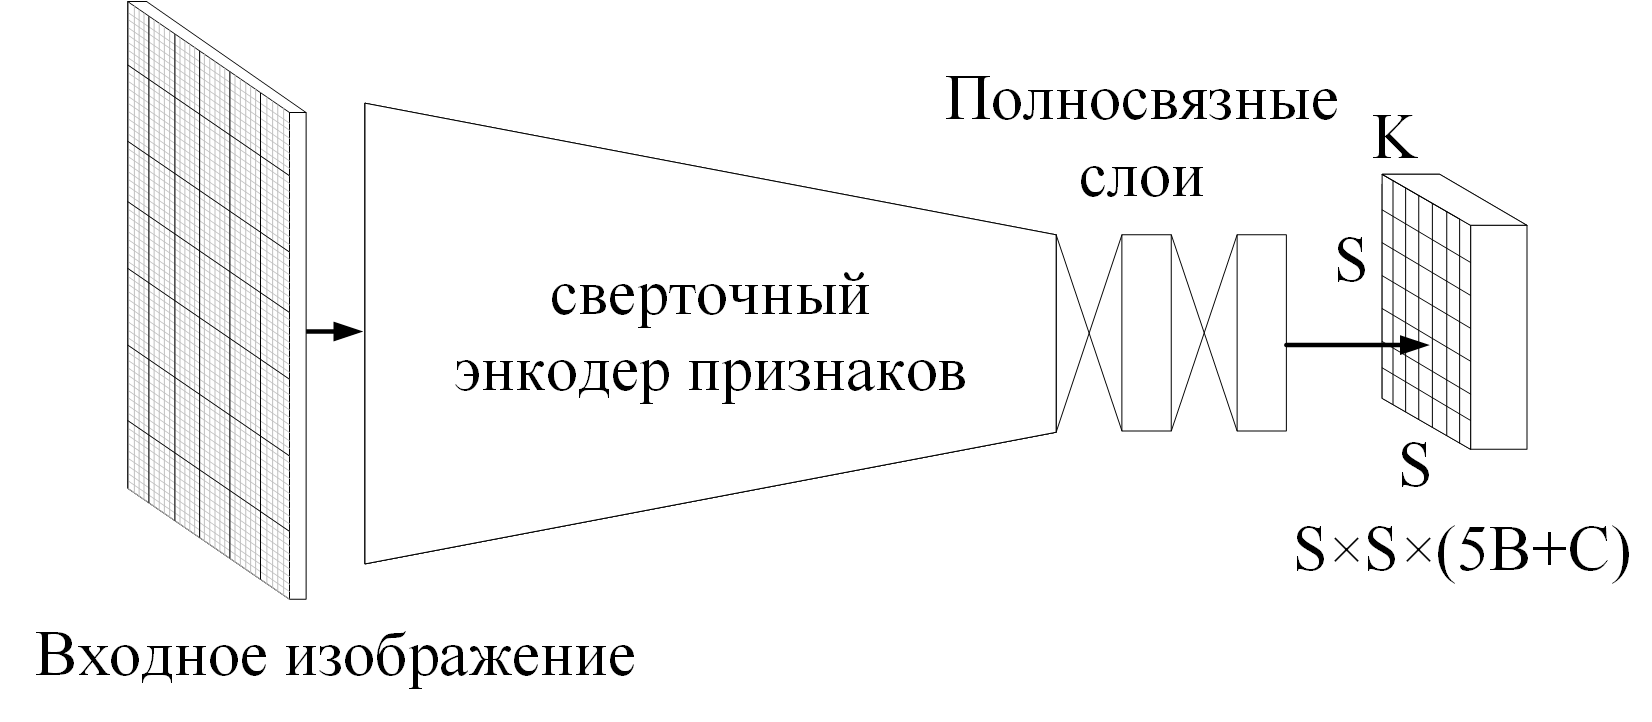
\includegraphics[width=0.99\linewidth]{./figuresch1/YOLO.png}
    		\caption{Иллюстрация  принципа работы  архитектуры YOLO}	
    		\label{ch1:fig:R_CNN}
    	\end{center}
    \end{figure}
    
%%%%%%%%%%%%%%%%%%%%%%%%%%%%%%%%%%%%%%%
\subsubsection{Кратко о задачах генерации в компьютерном зрении}

Как правило в компьютерном зрении и других приложениях глубокого обучения нейронных сетей рассматриваются задачи в которых из входных данных выделяются некоторые признаки, на основании которых принимаются целевые решения. Такие задачи можно назвать \textbf{дискриминативные задачи} \cite{Nikolenko2017DL}.  Для разных экземпляров данных признаки могут быть регулярными (характерными), однако при этом они могу быть немного разными. Так например характерным признаком лица являются глаза, однако, расположение, форма и т.д. глаз у на разных фотографиях будут разными. Тогда можно сказать что нейронная сеть выучивает именно признак ни как конкретное число или набор чисел, а как конкретное распределение. Другими словами, признаки о которых идет речь можно рассматривать как не детерминированные - то есть стохастические (по существу, случайные) величины, которые обладают некоторым характерным распределением, имеющим характерное среднее значение и другие параметры.  При таком рассмотрении сети помимо дискременативной задачи можно также поставить задачу генерации не только ответа сети, но и самих признаков, формирующих целевой ответ. Другими словами задачу генерации случайных значений признаков, полученных из соответствующих признаку распределений. Например, если сеть выучила распределение признаков лица (глаза, нос, уши и т.д.), то мы можем генерировать случайное лицо из некоторого посевного случайного набора чисел. Тут посевным набором называется число, исходя из которого выбирается некоторый результат распределения (если представить распределение как $p(x)$, то $x$ - посевное число.  Описанные задачи называются \textbf{генеративные задачи (или порождающие задачи)} \cite{Nikolenko2017DL}. 

Цель обучения порождающей нейронной сети в наиболее общем виде - это минимизация различий между распределениям некоторых признаков входных данных и выходных данных генерируемых нейронной сетью. Например, если есть набор лиц людей, то порождающая нейронная сеть должна давать на выходе изображения лиц, в которых например распределение размеров глаз, их положений или цвета будет таким же как для входных данных. Однако, так как на входе у нас есть только некоторые дискретные примеры лиц - то есть частные случае распределений, которые должна выучить сеть, то за счет обобщающею способности сеть может давать и другие частные случае распределений - случаи, которых нет во входных данных. Отметим, что на этом примере хорошо видно, что при обучении сеть аппроксимирует распределения признаков по их частным значениям. При этом эти аппроксимации формируются именно за счет связанных нелинейных преобразований входных данных. 
Отметим, что в зависимости от конкретных случаев обучение порождающей нейронной сети может производится как с учителем, так и на неразменных данных (unsupervised) или на данных с частичной разметкой (semi-supervised) \cite{Nikolenko2017DL}.

Современные глубокие \uline{генерирующие модели могут быть разделены на два класса - модели с явным представлением распределения признаков и модели со скрытым представлением} \cite{goodfellow2016nips}. Наиболее популярен второй класс \cite{Nikolenko2017DL}. Среди подходов первого вида следует выделить модели, основанные на автоэнкодерах, в частности \textbf{вариационный автоэнкодер (Variational Auto Encoder, VAE)} \cite{kingma2013auto}. Модель VAE представляет собой модификацию обычной автокодирующей сети (автоэнкодера, см. рисунок ~\ref{ch1:fig:autoencoder}). Однако, в VAE кодирующая часть (энкодер) создает не непосредственно скрытое пространство, а пытается его аппроксимировать  гауссовыми распределениями, для этого модель энкодера пытается оценить среднее и дисперсию для каждого параметра. Таким образом, создается как-бы распределение параметров. Затем из распределений создается входной вектор для декодирующей части из которого должен получиться ответ, в соответствующий распределению входных данных. Другими словами VAE должен генерировать новый результат на выходе - результат не похожий на входной экземпляр данных (как для обычного автоэенкодера), но из того же распределение что и экземпляр входных данных. По существу, такой подход соответствует идеи вариационного вывода, известной в других областях машинного обучения \cite{ghojogh2021factor}. В литературе предложено достаточно большое количество модификаций идеи VAE для решения задач компьютерного зрения \cite{asperti2021survey, harshvardhan2020comprehensive}. Также идеи вариационного вывода, и VAE в частности, используются в генерации текстов \cite{wang2019t} и как решение задачи анализа временных рядов \cite{fortuin2020gp} и потока видеоданных \cite{walker2016uncertain}. 

Отмечается, что основной недостаток подхода VAE - характерное гауссово размытие результатов работы \cite{ harshvardhan2020comprehensive}. Однако, влияние данного эффекта может быть снижено, например, путем использования  дополнительных нейронных сетей, создающих дополнительные условия контрастности при обучении \cite{mescheder2017adversarial}.

В 2014 году в работе \cite{goodfellow2014generative} Яном Гудфеллоу и соавторами, в том числе Йошуа Бенджо была предложена архитектура \textbf{генеративно-состязательная нейронная сеть (ГАН, Generative-Adversel Neural Network, GAN).} Архитектура представляет собой класс моделей со скрытым представлением и является наиболее популярным подходом к задачам генерации. 

\uline{Основная идея архитектуры заключается в использовании двух сетей - генерирующей (generative) и дискриментаивной (discriminative), которые обучаются совместно}.  Цель генеративной сети заключается в создании изображения из входных - посевных данных, которыми могут быть как случайный шум, так и некоторая разметка желаемого результата. На вход дискреминативной сети попеременно передаются данные, сгенерированные сетью (поддельные - fake данные) и примеры реальных данных, соответствующих, требуемой задачи. Например, изображения лиц - реальные данные (real). Цель дискреминативной сети определить поддельные или реальные данные поданы на ее вход. Таким образом, цель обучения архитектуры ГАН - одновременно понизить погрешность генеративной сети и повысить погрешность дискреминативной сети. Другими словами нужно сделать так, чтобы дискреминативная сеть не смогла определить какие данные поданы на ее вход - реальные или поддельные. При достижении этой цели можно предположить, что генеративная сеть смогла достоверно аппроксимировать распределения признаков, соответствующих задаче. Сеть называется генеративно-состязательной, так как, при обучении ГАН происходит одновременно попытка понижения ошибки генерирующей сети и попытка повышения ошибки дискреминативной сети. Отметим, что в связи с вышесказанным дискреминативная сеть может рассматривается как метод регуляризации работы генеративной сети. Иллюстрация работы архитектур ГАН приведена на рисунке \ref{ch1:fig:GAN}.

    \begin{figure}[!h]
    	\begin{center}
    		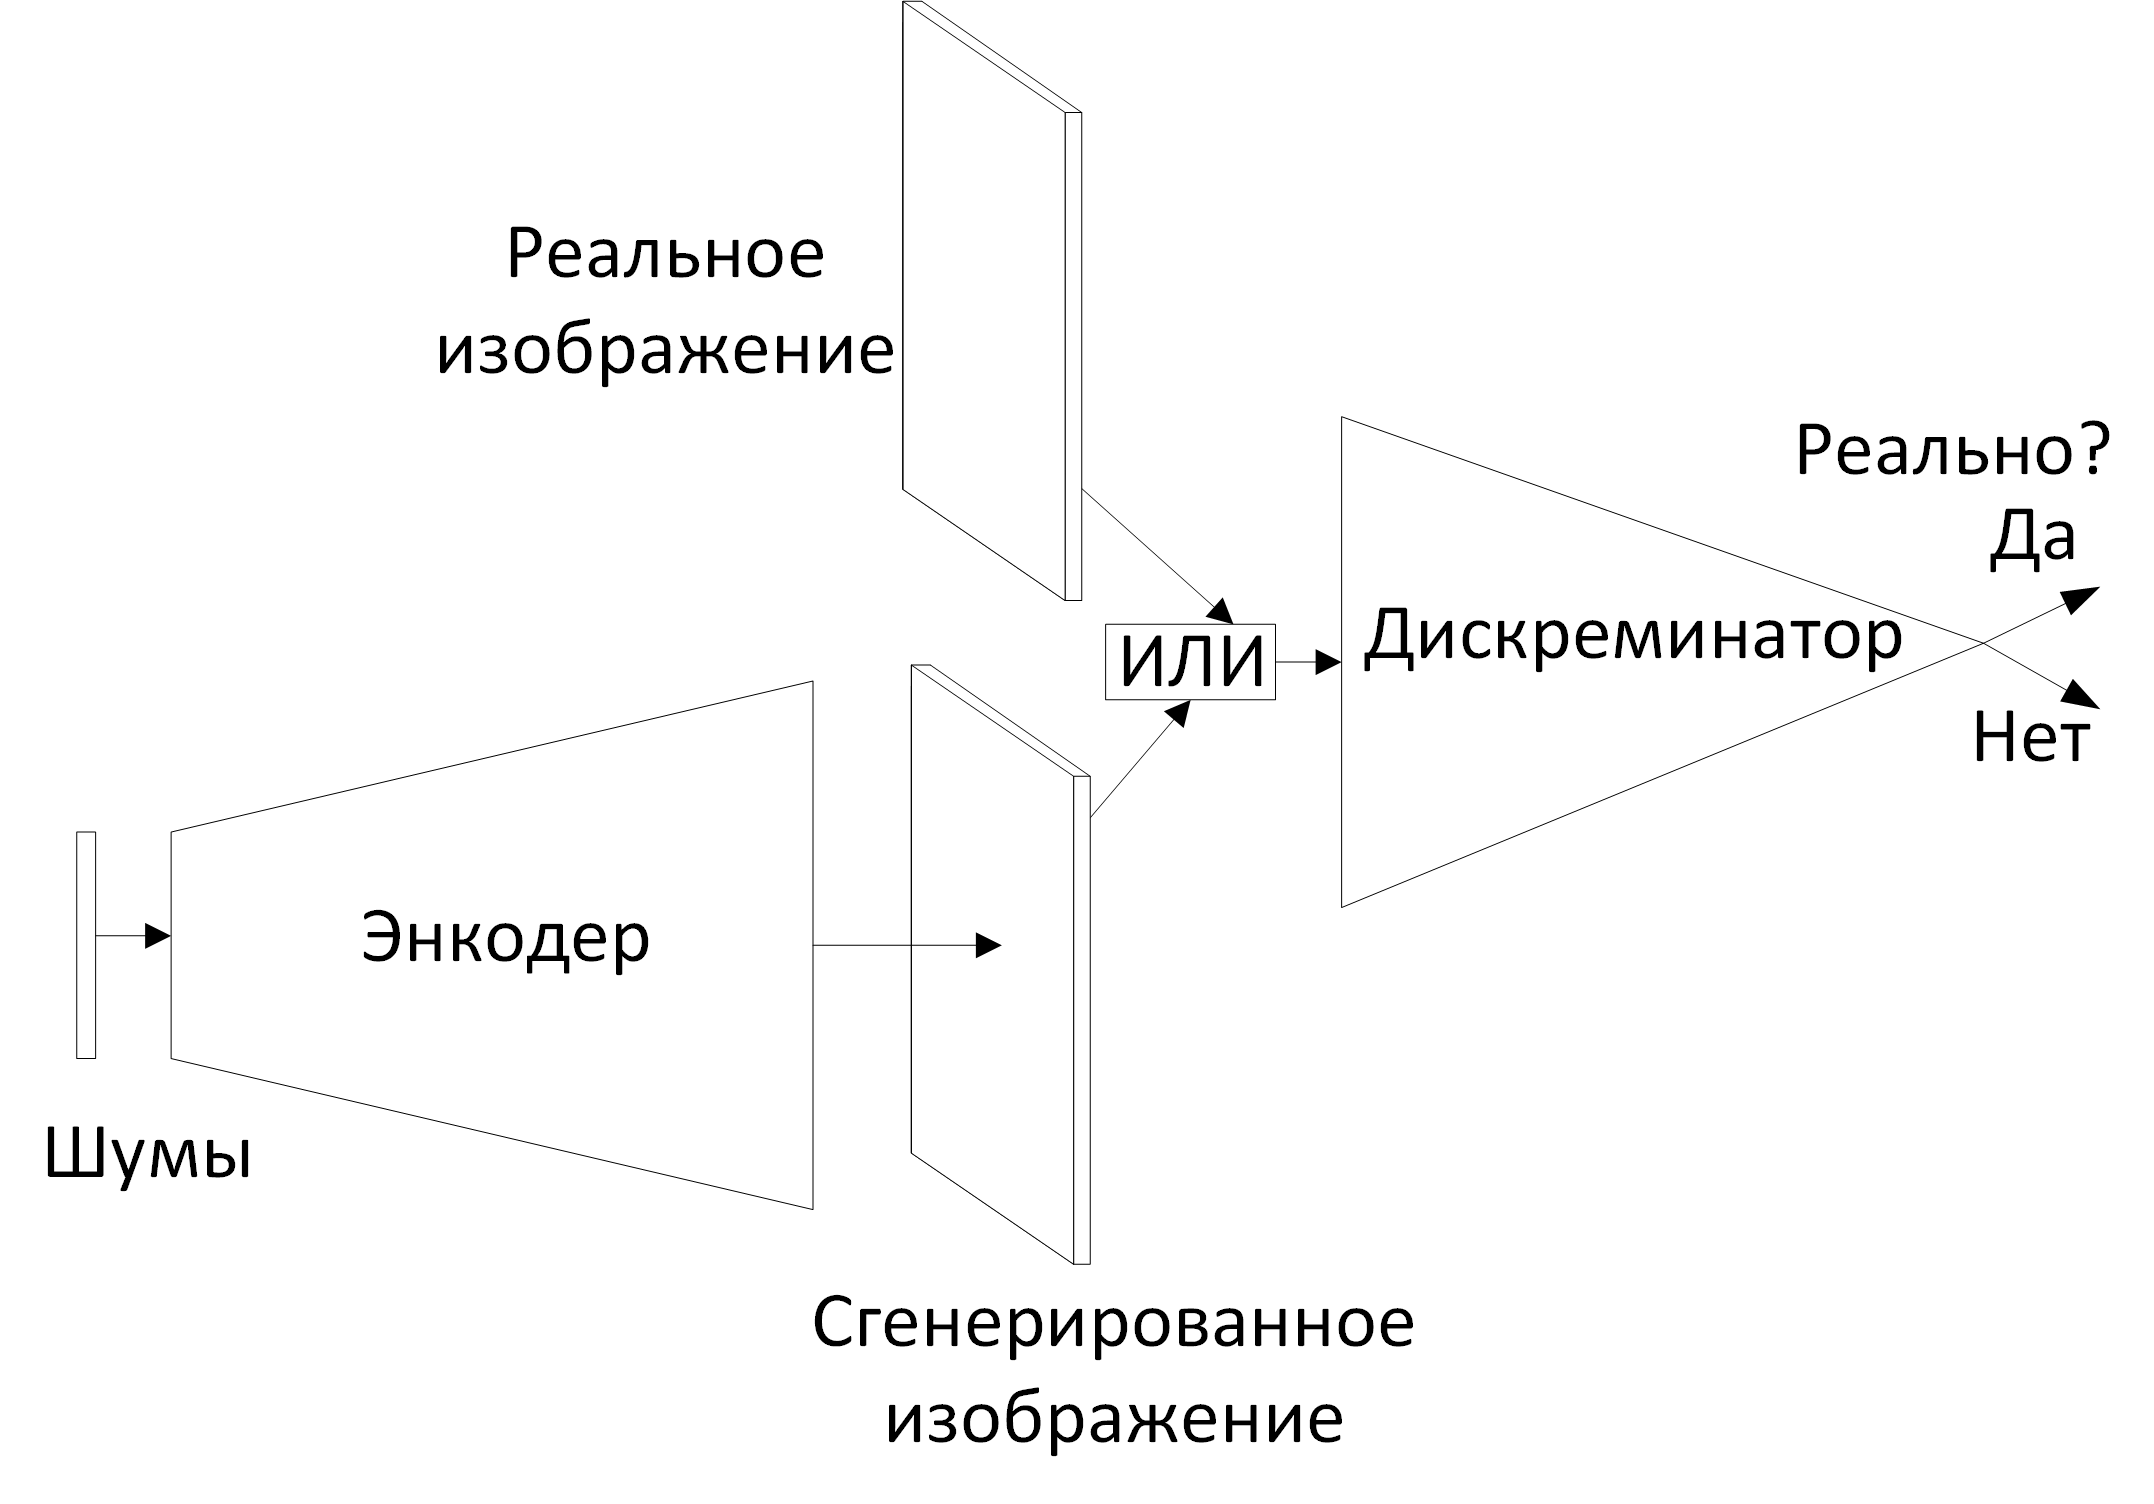
\includegraphics[width=0.99\linewidth]{./figuresch1/GAN.png}
    		\caption{Иллюстрация  принципа работы  архитектуры GAN}	
    		\label{ch1:fig:GAN}
    	\end{center}
    \end{figure}
%TODO: картинка GAN

В оригинальной статье Гудфеллоу предлагалось обучать ГАНы без разметки данных (то есть без учителя), при этом данные должны были генерироваться из шума. Однако, позже были предложены различные варианты реализации подхода как для задач работы с изображениями, так и для задач генерации текстовых данных, музыки \cite{gui2020review} и в других, более экзотических, приложениях \cite{manaswi2020generative, jabbar2020survey}. В 2016 году Гудфеллоу была опубликована работа \cite{goodfellow2016nips}, в которой было подробно проанализировано место подхода ГАН среди других подходов к генеративному обучению и были даны подробные разъяснения касательно аспектов функционирования ГАН.

В работе \cite{goodfellow2016nips}  Гудфеллоу были обозначены следующие возможные цели создания и развития архитектур глубоких нейронных сетей генеративного обучения.
\begin{itemize} \itemsep 0em
    \item Обучение и выборка из генеративных моделей является перспективным методом проверки способности  представлять и управлять многомерными распределениями вероятностей. Распределения вероятностей многомерных данных являются важными объектами в широком спектре прикладных математических и инженерных областей.
    \item Использование генеративного подхода в обучении с подкреплением в качестве генератора входной среды. При этом также может быть получена статистика и по самой модели - путем проверки ее поведения в различных вариантах ситуаций одного типа.
    \item Использование генеративного подхода в качестве метода предсказания нескольких вариантов по текущим данным (например для временного ряда или видео ряда) - то есть для задач с мультимодальным выходом.
    \item Использование генеративного подхода в качестве метода обучения данных с пропусками. Например, для обучения с полу-учителем, для поиска аномалий или для решения проблем несбалансированных данных - когда данных одного класса в несколько раз больше чем другого. Например, в случае двух классов, когда размечен только один класс или часть данных - для известного класса обучается ГАН, а затем обученный дискреминатор используется для разметки остальных данных. 
    \item Использование генеративного подхода для повышения разрешения входных данных - т.н. задача super-resolution.
    \item Решение задач типа перевод одного изображения  в другое (Image-to-image translation). Например преобразование некоторой зарисовки или шаблона в конечное изображение.
\end{itemize}

Отметим, следующие перспективные задачи, решаемые генеративными нейронными сетями и не вошедшие в список выше. В 2017 году был описан метод аугментации данных при помощи ГАН \cite{antoniou2017data}. В 2016 году была предложена идея генерации из текст в изображение (изображающее описанное в тексте) при помощи ГАН \cite{reed2016generative} и наоборот (изображение в текст) \cite{he2017deep}. В ряде работ предлагаются архитектуры для генерации изображений на основании семантически набросков \cite{park2019semantic} или при помощи переноса признакового пространства из одной задачи в другую.  Подход ГАН может быть использован для повышения устойчивости к изменениям данных при обучении нейронных сетей  - то есть к т.н. соревновательным атакам \cite{bai2020ai}. Также,  отметим, что одним из первых успешных применений архитектур - трансформеров в компьютерном зрении было их использование в генеративных задачах \cite{parmar2018image}. 

Как правило, на практике подход ГАН подход оказывается более точным, чем VAE и другие генеративные подходы. Однако, в некоторых случаях, например \cite{vahdat2021score}, арихтекутры на основе VAE оказываются более точными. Отметим, что в литературе рассматриваются архитектуры включающие совместно  ГАН и VAE подходы \cite{larsen2016autoencoding}. Также в ряде современных исследований переделаются  VAE-подобные подходы, которые, как указывается, разрешают основные проблемы ГАН архитектур и потенциально позволяют достичь больших точностей, чем способны ГАН \cite{dhariwal2021diffusion}. 

В последние несколько лет также встречается большое количество работ, где генеративные нейронные используется для генерации текстовых данных \cite{iqbal2020survey}. Однако, указывается что на данный момент это направление, особенно в случае подхода ГАН,  имеет ряд недостатков, связанных с, по существу, дискретной природой текста, а классическое генеративное обучение строит непрерывные аппроксимации признакового пространства. Другими словами, например, для генерации изображений лиц, распределение ширины глаз должно быть непрерывным. Для текста непрерывное распределение не подходит, так как осмысленные грамматически верные слова - представляют собой дискретные значения признаков. В литературе рассматриваются несколько вариантов решения данной проблемы, однако не один из них не является зарекомендовавшим себя по настоящее время \cite{hossam2021text, iqbal2020survey}. Также генеративное обучение, в частности ГАН, могут быть использованы при синтезе музыкальных композиций,   \cite{kulkarni2019survey} и при анализе временных рядов \cite{hartmann2018eeg}.

%%%%%%%%%%%%%%%%%%%%%%%%%%%%%%%%%%%
\newpage
\subsection{Современные тренды - итоги исторического обзора}

Глубокое обучение нейронных сетей, в том числе сверточных нейронных сетей получило широкое развитие в различных приложениях компьютерного зрения. Большинство фундаментальных результатов в этой области были получены в период конца 1990-х - 2015 годах. Однако, большая часть решений в их современном виде (архитектуры слоев и их блоков, методы регуляризации, типы функций активации скрытых слоев и т.д.) были разработаны после 2010-2012 годов. Так, например, общий подход к построению архитектуры сверточных нейронных сетей начинается с AlexNet. При этом иронично то, что и современные реализации LeNet 5 по сути представляют собой модификацию AlexNet.
В обозначенный период времени утвердились такие решения, как:
\begin{itemize} \itemsep 0.1em 
    \item построение архитектур на основании блоков, включающих сверточные слои, слои пулнга, слои внимания и остаточные связи; 
    \item регуляризация обучения путем батч-нормализации или методом дропаутов (
    \textcolor{red}{а также адаптивные методы обучения о которых речь пойдет в свое время)}; 
    \item предпочтительность использования автоматизированных методов подбора архитектур для конечных конфигураций аппаратного обеспечения и задачи;
    \item предпочтительность инициализации параметров путем предобучения нейронных сетей на больших наборах данных или на нескольких объединённых наборах данных.  
\end{itemize}

\noindent При этом по настоящее время открытыми остаются следующие вопросы.
%%%%%%%%%%%%%%%%%%%%%%%%
\newline

%%%%%%%%%%%%%%%%%%%%%%%%
\noindent\textbf{Выбор структуры блока сверточной сети и стратегии автоматической оптимизации}

В научной литературе предложены достаточно большое количество вариантов построения блоков сверточных слоев. В некоторых случаях такие блоки ориентированы на их использование в специализированном оборудовании (например, для процессоров мобильных телефонов). В других случаях, блок должен быть универсальным. В зависимости от предназначения оптимальная структура блока может меняться. При этом вопрос о том, какой структура должна быть в тех или иных случаях остается не решенным. 
Отметим, что часто можно встретить мнение о том, что оптимальная архитектура нейронной сети (или ее блока) может быть выбрана методами автоматического поиска (например, NAS). Однако, следует помнить, что NAS позволяет провести оптимизацию только по выбранному пространству. Другими словами даже такие методы ограничены опытом исследователи и знаниями об эффективных структурах сверточных и других блоков. Кроме того в отношении NAS всегда следует помнить о корректности выбранной стратегии поиска и корректности выбранных критериев оценки качества модели.
%%%%%%%%%%%%%%%%%%%%%%%%
\newline
%%%%%%%%%%%%%%%%%%%%%%%%
\noindent\textbf{Выбор методов регуляризации обучения и работы нейронной сети} 
Как было указано выше метод батч-нормализации является одним из основных методов регуляризации обучения нейронных сетей. Метод имеет ряд достоинств, в том числе \cite{brock2021high}: 
\begin{itemize} \itemsep 0.05em 
    \item снижение эффекта ковариационного сдвига и увеличение обобщающей способности; 
    \item \textcolor{red}{ускорение обучения за счет правильного диапазона значений функции активации - устранение т.н. "mean-shif" эффекта для ранних эпох обучения}; 
   \item  возможность увеличения размеров батча и более грубого выбора скорости обучения. 
\end{itemize} 
Однако, условия для работоспособности метода батч-нормализации не всегда удается выполнить, о чем отмечают многие авторы \cite{moradi2020survey, huang2020normalization, brock2021high}. 
В качестве основных мотивов для использования альтернативных методов нормализации 
% в работе  \cite{brock2021high} 
приводятся следующие недостатки классической батч-нормализации:
\begin{itemize} \itemsep 0.05em  
    \item несоответствие результатов работы во время обучения и работы нейронной сети, а также в случаях предобучения и дообучения на пакетах разного размера или наборах данных с разным размером входных изображений;
    \item батч-нормализация не оказывает регуляризирующего эффекта для небольших размеров мини-пакетов (порядка нескольких экземпляров данных);
    \item при длительном обучении сетей с остаточными связями батч-нормализация приводит к преобладанию остаточных связей в слоях (снижает точность обучения).
    % \item батч-нормализация нарушает предположение о независимости экземпляров данных для каждого мини-пакета;
    % \item увеличение вычислительной сложности и требований к памяти для хранения параметров батч-нормализации.
\end{itemize}
В случаях, когда батч-нормализация не применима могут быть использованы альтернативные подходы\cite{huang2020normalization}. Также открытым остается вопрос о том, что лучше: метод дроп-аутов или батч-нормализация. Отметим, что и в дополнение к данным методам нейронные сети всегда могут быть обучены с использованием классической L1/L2 регуляризации и с использованием аугментации данных. Однако, в работе \cite{van2017l2} показано, что L2 регуляризация почти не дает результата в случае батч-нормализации. А в работе \cite{srivastava2014dropout} показано, что L2 улучшает работы метода дропаутов. 
Отметим, что в работе 2020 года \cite{zhong2020random} показано,  что аугментация данных методом случайного удаления частей изображений соответствует принципу работы метода дропаутов. Также данный подход вероятно может быть применен совместно с батч-нормализацией. 

В 2020 году командой Google Deep Mind была предложена модификация архитектур ResNet и EfficientNet c оригинальным пересмотром идеи слоя батч-нормализации \cite{brock2021characterizing, brock2021high}. Архитектуры разработанной нейронной сети было предложено называть NFNet \cite{brock2021high}. 
Авторы NFNet смогли достичь точности 97.9\% по "top-5" и  86.5\% по методу "top-1" для набора данных ImageNet без использования дополнительных данных для предобучения. 
\textcolor{red}{
Для нейронных сетей без предобучения на дополнительных данных - это наивысший результат на начало августа 2021 года.
\cite{paperswithcodeImagenet}}.
%%%%%%%%%%%%%%%%%%%%%%%%
\newline

%%%%%%%%%%%%%%%%%%%%%%%%
\noindent\textbf{Оптимизация стратегий обучения глубоких нейронных сетей}

В 2019 наилучший результат для набора данных ImageNet показала архитектура BiT - вариант архитектуры ResNet c расширенными слоями (увеличено число карт признаков) и предобученный на наборе данных  JFT-300M (300 миллионов изображений, \cite{sun2017revisiting}) при помощи специальных правил BiT-HyperRule \cite{kolesnikov2020big}. Архитектура показала точность 98,5\% по "top-5" и 88 \% по методу "top-1" \cite{paperswithcodeImagenet}. Пример архитектуры BiT показал, что при условии достаточного предобучения возможно расширение слоев нейронных и увеличение обобщающей способности. Однако, оставил открытым вопрос о том, каким образом лучше проводить предобучение.
Отметим, что помимо классического предобучения с использование больших наборов данных в современной литературе исследуются следующие методы оптимизации обучения:
\begin{itemize} \itemsep 0.1em 
    \item обучение со смешиванием экземпляров данных и их меток \cite{shorten2019survey};
    \item обучение с добавлением шумов к меткам (lable smoothing \cite{muller2019does});
    \item обучения с использованием дополнительной нейронной сети - методы "учитель-ученик" 
    (относят к классу т.н. методов полу-контролируемого обучения, Semi-supervised Learning) \cite{yang2021survey}; 
    \item методы само-предобучения (Self-Supervised Learning) \cite{liu2021self}.  
\end{itemize}

Среди методов смешивания данных и меток следует выделить работы 2017 и 2019 годов, в которых исследованы методы аугментации MixUp - наложение изображений и сложение меток в соответствующих прозрачности пропорциях \cite{zhang2017mixup} и метод CutMix - вставка частей изображений и  и сложение меток в соответствующих площади пропорциях. Также различными авторами предлагаются модификации данных и других схожих методов \cite{shorten2019survey}.

Методы обучения "Учитель-Ученик" предполагают наличие двух нейронных сетей, которые в зависимости от техники обучения могут иметь разное соотношение размеров. Так, например, для популярной техники дисциляции знаний (Knowlege Distilation) предполагается, что сеть-учитель (или ансамбль сетей) имеют больший размер, по сравнению с целевой сетью - учеником.  Целью такого обучения является подстраивание результатов работы сети-ученика под результаты сети учителя. При этом предполагается, что сеть ученик также научится копированию поведения учителя в отношении обобщающей способности.
\cite{gou2021knowledge}

В 2020 наилучшие результаты для набора данных ImageNet показали архитектуры EfficientNet-B7 \cite{xie2020self}, и EfficientNet-L2 \cite{pham2021meta}, предобученные и тренированные разработанными вариантами методов учитель-ученик.  В случае EfficientNet-L2 проводилось обучение с полу-учителем, методом названным Meta-Pseudo-Labeling \cite{pham2021meta}. При этом авторы работы \cite{pham2021meta} достигли точности 98,2 \% по методу "top-5" и 90,2 \% по методу "top-1" \cite{paperswithcodeImagenet}. 
% В обоих работах \cite{xie2020self, pham2021meta} использовался принцип "ученик-учитель" - то есть две нейронные сети, одна из которых (Учитель) предобучалась и размечала набор данных для сети ученика. 
% \textcolor{red}{Подробности методов самообучения будут рассмотрены в книге далее}. 
% Указанные работы \cite{xie2020self, pham2021meta} катализировали дискуссию о необходимости и методах совершенствования схем обучения нейронных сетей. 
%%%%%%%%%%%%%%%%%%%%%%%%
\newline

%%%%%%%%%%%%%%%%%%%%%%%%
\noindent\textbf{Подходы к решению задач: трансформеры, полносвязные или сверточные сети} 

Как следует из обзора основной подход у решению задач компьютерного зрения - это использование глубоких сверточных нейронных сетей. Однако, работы 2020-2021, посвященные архитектурам-трансформерам показали перспективность подхода для больших наборов данных (на этапе предобучения) и при больших размерах экземпляров данных. Часть предложенных в литературе архитектур- трансформеров полностью полносвязные, часть имеют и сверточные и полносвязрые слои. Например в августе 2021 года была представлена архитектура BotNet. Авторы BotNet предложили заменить часть слоев архитектуры ResNet на слои многоголового само-внимания и при этом получили небольшой прирост точности (~0,5\%) по сравнению с оригинальной архитектурой, однако, они увеличили число параметров\cite{srinivas2021bottleneck}. Таким образом вопрос о том, какой подход (или комбинация подходов) - лучше остается открытым. В работе \cite{raghu2021vision} посвященной сверточных сетей и трансформеров приходят к выводу, что трансформеры быстрее и более точно выучивают крупно-размерные признаки, чем сверточные сети. Однако, архитектурам-трансформерам требуется больше примеров для мелко-размерных признаков. 

В 2021 году был представлен ряд трансформеров-подобных полносвязных архитектур для решения задач компьютерного зрения. В таких архитектурах соли многоголового само-внимания был заменены на наборы операций с полносвязными слоями \cite{guo2021can}. Наиболее известная из таких архитектур MLP-Mixer, предложенная командой Google Brain. Архитектура показала точность (87,9\% по методу top-1 на наборе данных ImageNet) с предобучением на наборе данных JFT-300M, показав при этом производительность в 2,5 раза выше, чем архитектура ViT \cite{tolstikhin2021mlp}.  На данный момент полностью полносвязные архитектуры не дают высокой точности, сопоставимой с трансформерами, однако потенциально способных их заменить. Основным преимуществом таких архитектур является пониженное число параметров (из за отсутствия многоголового само-внимания) и высокая скорость работы (операции с полносвязными слоями - самые быстрые).

Также отметим подход CLIP переставленный командой OpenAI в работе \cite{radford2021learning}. Авторы предложили проводить предобучение на набора изображений с описанием. В основе подхода лежит идея, что для набора обучаются два кодировщика признаков (один для изображения, другой для описания) так, чтобы они давали наиболее схожие представления на выходе. Таким образом, по задумке авторов, модель должна выучить текстовое описание для изображений. Авторы рекомендуют использовать в своем подходе архитектуры трансформеры. Подход интересен своей оригинальностью и возможно является перспективным. Главным достоинством подхода является высокая обобщающая способность. Однако, в настоящее время подход показывает достойные результаты лишь на некоторых задачах. 
% %%%%%%%%%%%%%%%%%%%%%%%%%%%%%%%%%%%%%%%%%%%%


% https://arxiv.org/pdf/2101.01169.pdf
% Since acquiring manual labels at a massive scale is cumbersome, self-supervised learning has been very effectively
% used in the pre-training stage. The self-supervision based
% pre-training stage training has played a crucial role in unleashing the scalability and generalization of Transformer
% networks, enabling training even above a trillion parameter networks (e.g., the latest Switch Transformer [10] from
% Google). An extensive survey on SSL can be found in [40],
% [41]. As nicely summarized by Y. LeCun [42], the basic
% idea of SSL is to fill in the blanks, i.e., try to predict the
% occluded data in images, future or past frames in temporal
% video sequences or predict a pretext task e.g., the amount
% of rotation applied to inputs, the permutation applied to
% image patches or the color of a gray-scale image. Another
% 4
% effective way to impose self-supervised constraints is via
% contrastive learning. In this case, nuisance transformations
% are used to create two types of modified versions of the same
% image i.e., without changing the underlying class semantics
% (e.g., image stylizing, cropping) and with semantic changes
% (e.g., replacing an object with another in the same scene, or
% changing the class with minor adversarial changes to the
% image). Subsequently, the model is trained to be invariant to
% the nuisance transformations and emphasize on modeling
% minor changes that can alter semantic labels.
% Self-supervised learning provides a promising learning
% paradigm since it enables learning from a vast amount of
% readily available non-annotated data. In the SSL based pretraining stage, a model is trained to learn a meaningful
% representation of the underlying data by solving a pretext
% task. The pseudo-labels for the pretext task are automatically generated (without requiring any expensive manual
% annotations) based on data attributes and task definition.
% Therefore, the pretext task definition is a critical choice in
% SSL. We can broadly categorize existing SSL methods based
% upon their pretext tasks into (a) generative approaches which
% synthesize images or videos (given conditional inputs), (b)
% context-based methods which exploit the relationships between image patches or video frames, and (c) cross-modal
% methods which leverage from multiple data modalities.
% Examples of generative approaches include conditional generation tasks such as masked image modeling [35] and
% image colorization [43], image super-resolution [44], image
% in-painting [45], and GANs based methods [46], [47]. The
% context-based pretext methods solve problems such as a
% jigsaw puzzle on image patches [48]–[50], masked object
% classification [22], predict geometric transformation such as
% rotation [38], [51], or verify temporal sequence of video
% frames [52]–[54]. Cross-modal pretext methods verify the
% correspondence of two input modalities e.g., text & image
% [55], audio & video [56], [57] or RGB & flow [58]

% http://proceedings.mlr.press/v139/touvron21a/touvron21a.pdf
% Knowledge Distillation (Hinton et al., 2015) refers to the
% training paradigm in which a student model leverages “soft”
% labels coming from a strong teacher network. This is the
% output vector of the teacher’s softmax function rather than
% just the maximum of scores, wich gives a “hard” label. Such
% a training improves the performance of the student model
% (alternatively, it can be regarded as a form of compression of
% the teacher model into a smaller one – the student). On the
% one hand the teacher’s soft labels will have a similar effect
% to labels smoothing (Yuan et al., 2020). On the other hand as
% shown by Wei et al. (2020) the teacher’s supervision takes
% into account the effects of the data augmentation, which
% sometimes causes a misalignment between the real label
% and the image. For example, let us consider image with a
% “cat” label that represents a large landscape and a small cat
% in a corner. If the cat is no longer on the crop of the data
% augmentation it implicitly changes the label of the image.
% Knowledge distillation can transfer inductive biases (Abnar
% et al., 2020) in a soft way in a student model using a teacher
% model where they would be incorporated in a hard way. In
% our paper we study the distillation of a transformer student
% by either a convnet or a transformer teacher, motivated by
% inducing convolutional bias into transformers.

% ВОЗМОЖНО СЛЕДУЕТ ПЕРеНЕСТИ ДАЛЬШЕ
% Как было сказано \textcolor{red}{выше (см. LeNet)} наиболее важной задачей разработки архитектур глубоких нейронных сетей является оптимизация кодировщика признаков (энкодера, см. рис. \ref{ch1:fig:LeNet5}). Такая задача эквивалентна задаче оптимизации представления данных. Мы уже рассматривали несколько способов оптимизации,  в том числе предобучение весовых параметров нейронных сетей и аугментация наборов данных. Однако пул методов в данной области гораздо шире.  
% \beg
% предобучение весовых параметров нейронных сетей на крупных наборах данных и перенос обучения. 


% (вы нейронных сетей на и т.н. \textbf{перенос обучения (transfer learning)} (переноса весовых параметров, оптимизированных для одной задачи на другую) развивались сообществом исследователей нейронных сетей по крайней мере с начала 1990-х \cite{zhuang2020comprehensive}. \ulune{Как правило перенос обучения предполагал, предобучение весовых параметров архитектуры на достаточно большом наборе данных и затем оптимизация и дообучение архитектуры для целевой задачи}. Таким образом, 

% https://sh-tsang.medium.com/reading-pnasnet-progressive-neural-architecture-search-image-classification-1beb1de06fe6
% https://library.oapen.org/bitstream/handle/20.500.12657/23012/1007149.pdf
% https://arxiv.org/pdf/1712.00559.pdf
% https://sh-tsang.medium.com/reading-pnasnet-progressive-neural-architecture-search-image-classification-1beb1de06fe6
% https://sh-tsang.medium.com/review-nasnet-neural-architecture-search-network-image-classification-23139ea0425d
% https://openaccess.thecvf.com/content_cvpr_2018/papers/Zoph_Learning_Transferable_Architectures_CVPR_2018_paper.pdf
% https://arxiv.org/pdf/1808.05377.pdf
% https://lilianweng.github.io/lil-log/2020/08/06/neural-architecture-search.html
% https://www.sciencedirect.com/science/article/abs/pii/S0950705120307516

% https://lilianweng.github.io/lil-log/2020/08/06/neural-architecture-search.html
% https://www.automl.org/automl/literature-on-neural-architecture-search/
% An Introduction to Neural Architecture Search for Convolutional Networks - https://arxiv.org/abs/2005.11074
% Neural architecture search: A survey - https://www.jmlr.org/papers/volume20/18-598/18-598.pdf
% Neural Architecture Search 1st lightweight NAS challenge-https://cvpr21-nas.com/
% https://sh-tsang.medium.com/overview-my-reviewed-paper-lists-tutorials-946ce59fbf9e
\section{EOC}
ГЛАВНОЕ ПРИЕМУЩЕСТВО DL; выделение, преобразование и выбор признаков, релевантные поставленной задачи.  Однако процедура обучения требует достаточно большого набора данных для правильной обработки таких  признаков 

%============================================%
% \newpage
% \section{!!!!!!!!!!!!!дальше}
% 1. Адаптивный линейный элемент (Widrow and Hoff, 1960)
% 2. Неокогнитрон (Fukushima, 1980)
% 3. GPU-ускоренная сверточная сеть (Chellapilla et al., 2006)
% 4. Глубокая машина Больцмана (Salakhutdinov and Hinton, 2009a)
% 5. Сверточная сеть без учителя (Jarrett et al., 2009)
% 6. GPU-ускоренный многослойный перцептрон (Ciresan et al., 2010)
% 7. Распределенный автокодировщик (Le et al., 2012)
% 8. Сверточная сеть с несколькими GPU (Krizhevsky et al., 2012)
% 9. Сверточная сеть без учителя на компьютерах типа COTS HPC (Coates et al., 2013)
% 10. GoogLeNet (Szegedy et al., 2014a)



% В случае слоя 2 на рис. \ref{ch1:fig:convnet1989} под ядром свертки подразумевается ядро размером $5\times 5\times 8$, где $5\times 5$ - размер каждого двухмерного ядра, а $8$ - число таких ядер в одном тензоре.  В случае трехмерного тензора операция свертки будет иметь вид:

% \begin{equation}
%     \label{ch1:eqn:conv}
%     r[i,j] = (k\ast x)[i,j] = \sum_{c=0}^{C-1}\sum_{a=0}^{h_k-1}\sum_{b=0}^{w_k-1}k[ c,a,b]x[c,i+a,j+b], 
% \end{equation}

% где 

% \begin{itemize}
% \item $C$ - число каналов свертки; 
% \item $k[c,a,b]$ - значение канала $c$ ядра свертки с координатами $[a,b]$ ($k$ имеет размерность $c \times h_k \times w_k)$;
% \item $x[c, i,j]$ - значение канала $c$ входного массива с координатами $[i,j]$ ($x$ имеет размерность $C\times h_x \times w_x$);
% \end{itemize}

% Иллюстрация образования одного двухмерного результата свертки вида (\ref{ch1:eqn:conv}) приведена на рисунке \ref{ch1:fig:conv_1channel}. Отметим также, что технически, к каждому ядру свертки должно быть добавлено слагаемое смещения. Таким образом полное описание структуры слоя 2 на рисунке  \ref{ch1:fig:convnet1989} требует введение следующих обозначений:

% \begin{equation}
%     \label{ch1:eqn:conv_3d}
%     r[c_{out}, i,j] = (k\ast x)[c_{out},i,j] = \sum_{c=0}^{C-1}\sum_{a=0}^{h_k-1}\sum_{b=0}^{w_k-1}k[c_{out}, c, a,b]x[c,i+a,j+b] + \theta[c_{out}], 
% \end{equation}

% где 

% \begin{itemize}
% \item $c_{out} = 0,...,C_{out}-1$ - число выходных карт признаков;
% \item $\theta[c_{out}]$ - смещение результата свертки ядра $k[c_{out},:,:,:]$ (каждого ядра);
% \item $r[c_{out}, i,j]$ - значение выходной карты признаков $c_{out}$;
% \item $k[c_{out}, c a,b]$ - 4-х мерный массив ядер свертки.
% \end{itemize}

% Иллюстрация образования нескольких карт признаков свертками вида (\ref{ch1:eqn:conv}) (см. выход слоя 2 на рис. \ref{ch1:fig:convnet1989}) приведена на рисунке \ref{ch1:fig:2d_conv}.
 
% \begin{figure}
% 	\begin{center}
% 		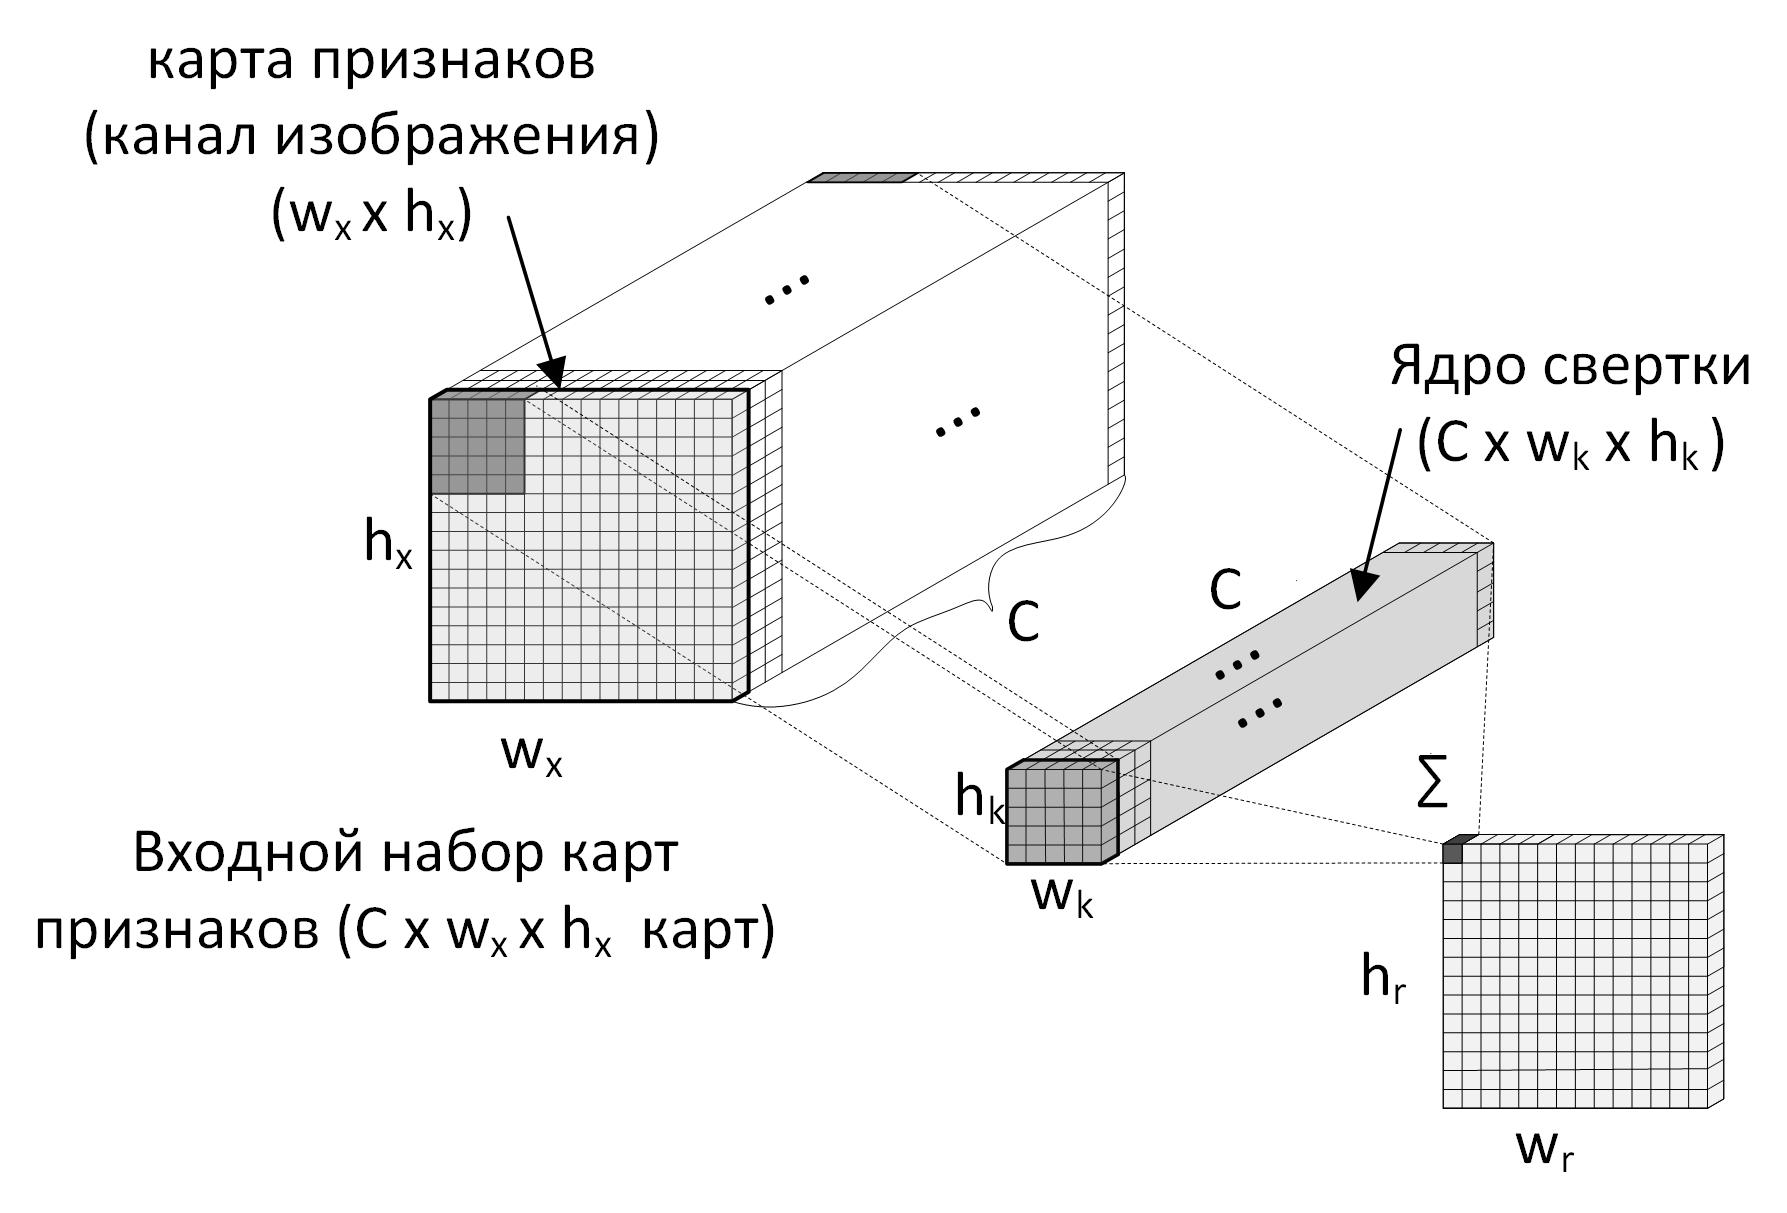
\includegraphics[width=0.7\linewidth]{./figuresch1/conv_1channel.png}
% 		\caption{Иллюстрация свертки вида (\ref{ch1:eqn:conv})}		
% 		\label{ch1:fig:conv_1channel}
% 	\end{center}
% \end{figure}
 
% \begin{figure}
% 	\begin{center}
% 		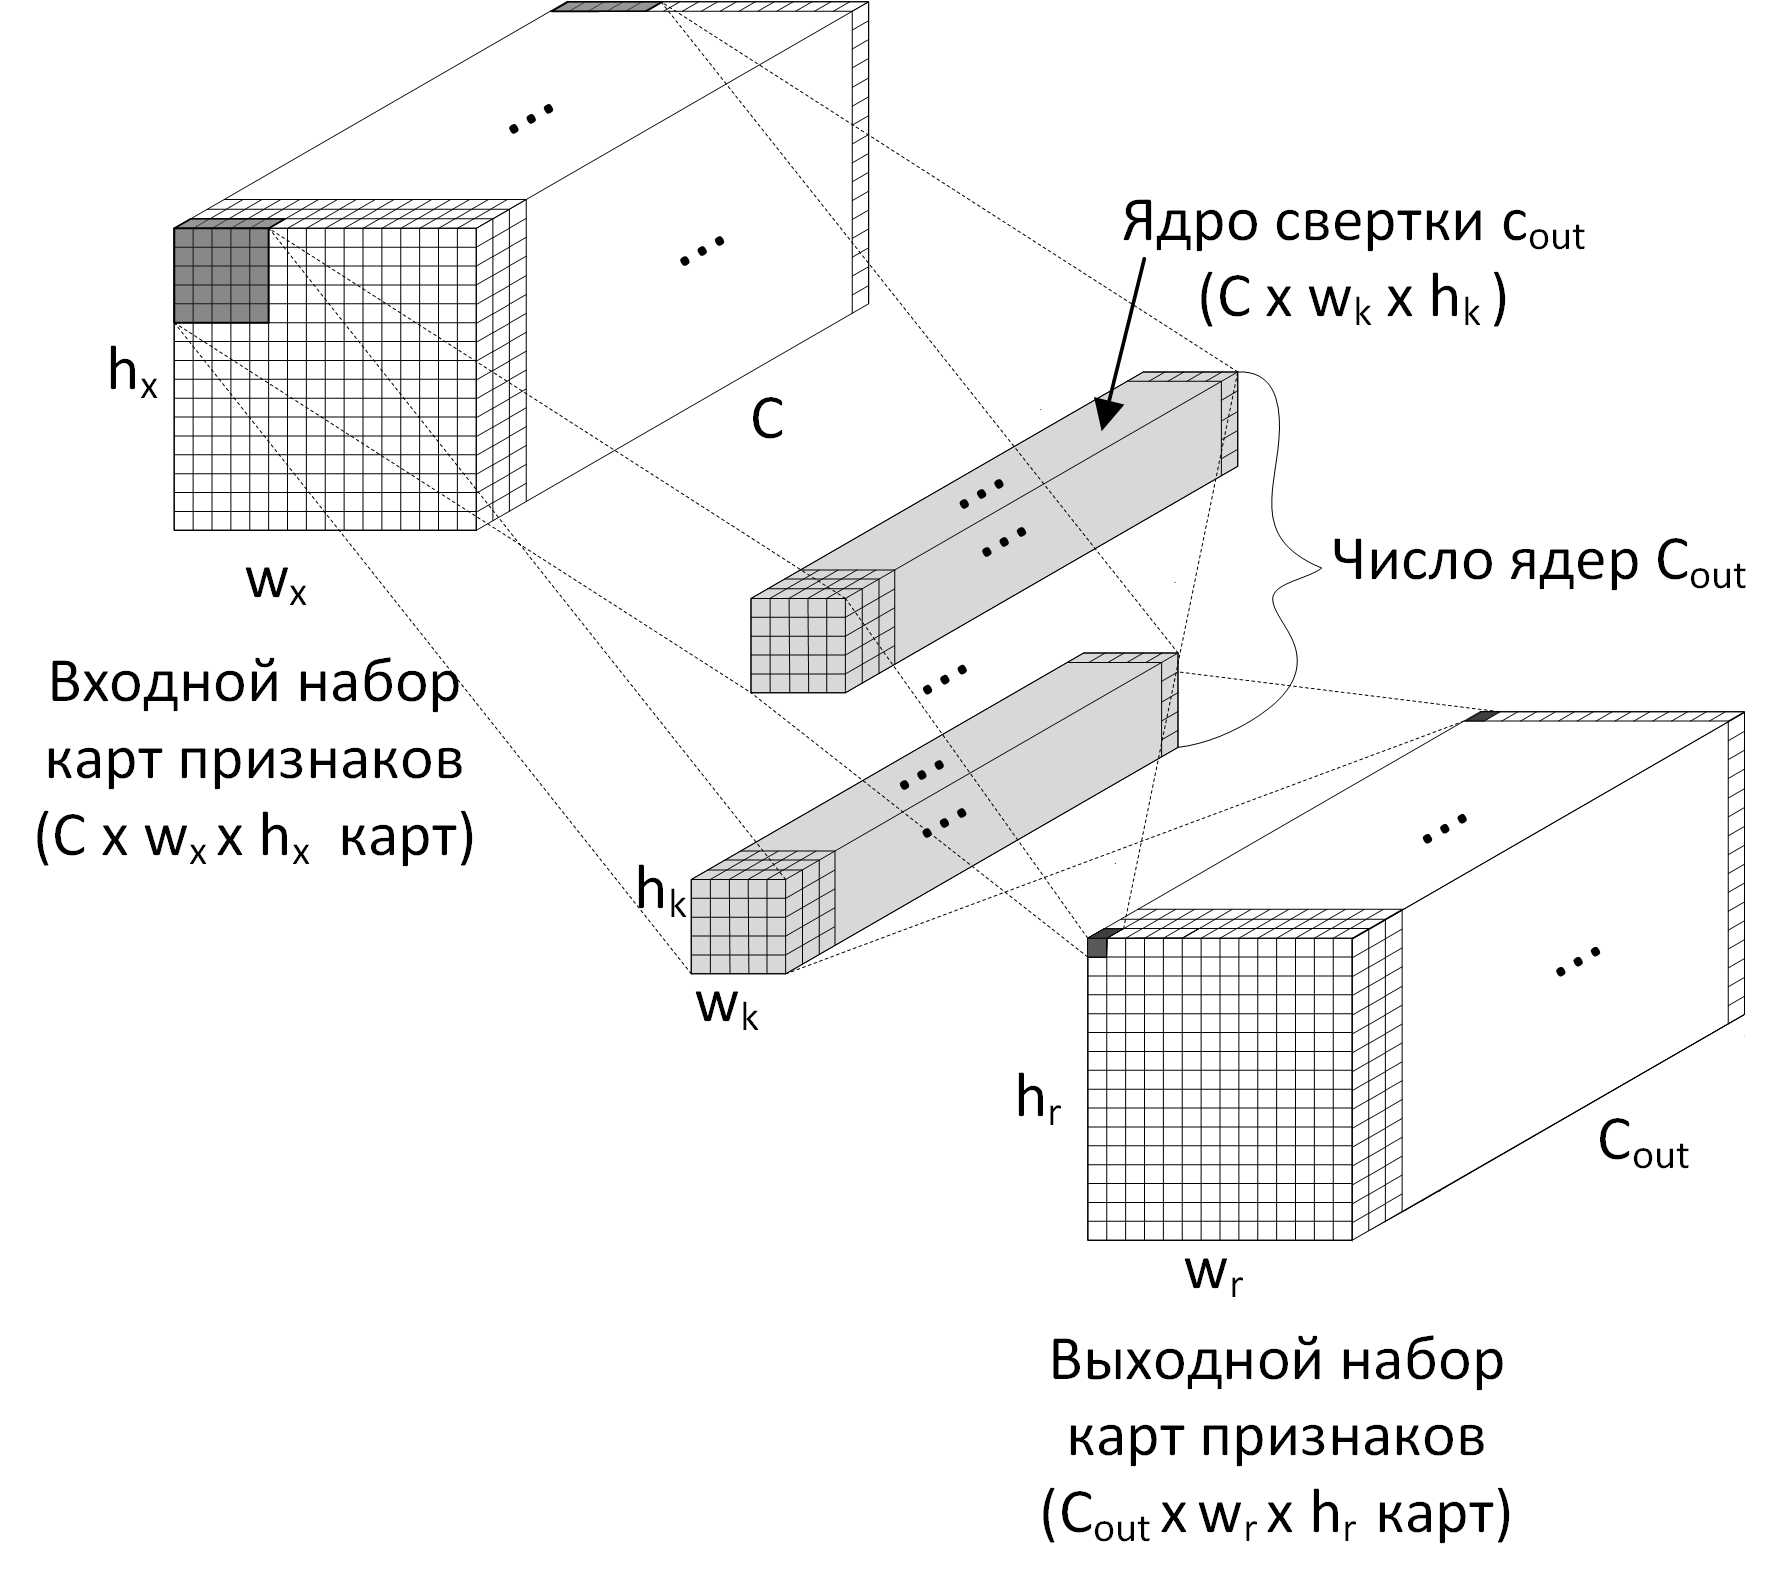
\includegraphics[width=0.7\linewidth]{./figuresch1/2d_conv.png}
% 		\caption{Иллюстрация образования выходной карты признаков для свертки вида (\ref{ch1:eqn:conv})}		
% 		\label{ch1:fig:2d_conv}
% 	\end{center}
% \end{figure}
 
% SIMD, SIMT,
% ссылки на вычислительный граф и бек проп и градиент
%https://m0nads.wordpress.com/2017/08/28/convolutional-neural-networks-part-2/
%https://medium.com/@zahraelhamraoui1997/the-convolutional-neural-network-theory-and-implementation-of-lenet-5-and-alexnet-5266e4577e96
%http://web.archive.org/web/20090630215858/http://evrika.tsi.lv/index.php?name=texts&file=show&f=410







% %%%%%%%%%%%%%%%%%%%%%%%%%%%%%%%%%%%%%%%%%%%%%  
% $$
% e = \frac{\partial L(y,\hat y)}{\partial \hat y} 
% \\\\
% w_i^{t+1}=w_i^{t}-\eta e f(o_i) 
% \\\\
% e_{ij} =(w_i e)
% $$


%  Пояснение работы метода обратного распространения ошибки может быть проведено для многослойного персептрона с одним скрытым слоем нейронов. Для такой модели можно записать результат работы нейронной сети в явном виде:
%  %%%%%%%%%%%%%%%%%%%%%%%%%%%%%%%%%%%%%%%%%%%%%
%  \begin{equation}
%  	\label{eqn:MLP_1Layer}
%  	\hat y = \sum_{i=0}^{P_1-1}w_{i} f(\sum_{j=0}^{P_0-1}w_{ji} x_j),
%  \end{equation}
%  где $\hat y$ - это результат работы нейронной сети; $w_1 = \{w_{i}\}$ и $w_0 =\{w_{ji}\}$ - наборы весовых коэффициентов для связи скрытого и выходного слоев $w_{i}$  и входного слоя  с каждым нейроном скрытого слоев  $w_{ji}$ соответственно; $x_j$ - входные признаки; число признаков $P_0$,  число нейронов скрытого слоя $P_1$; $f(\cdot)$ - функция активации.
%  %%%%%%%%%%%%%%%%%%%%%%%%%%%%%%%%%%%%%%%%%%%%%
%  Для вычисления направления антиградиента (и обновлений весов) необходимо записать производные \ref{eqn:MLP_1Layer} по каждому параметру наборов $w_0$ и $w_1$. 
%  Обозначим ошибку работу нейронной сети как $err = L(y,\hat y )$. 
%  Тогда вычисление значений градиента для набора весов $w_1$ можно выразить, используя \textbf{правило цепочек дифференцирования} в следующем виде:

%  %%%%%%%%%%%%%%%%%%%%%%%%%%%%%%%%%%%%%% 
%   \begin{equation}
%   	\begin{cases}
%  	\nabla_{w_1} err = \frac{\partial L(y,\hat y )}{\partial w_1} = 
%  	\left\{
%  	\frac{\partial L(y,\hat y)}{\partial \hat y}
%  	\frac{\partial \hat y}{\partial w_{i}}
%  	\right\}_{i=0}^{P_1},
%  	\\\\ 
%  	 \frac{\partial y}{\partial w_{i}} = 
%  	 f(\sum_{j=0}^{P_0-1}w_{ji} x_j)
%  \end{cases}
%   \end{equation}
%  %%%%%%%%%%%%%%%%%%%%%%%%%%%%%%%%%%%%%% 
 
%   Таким образом в результате дифференцирования получается вектор производных, по которым могут быть вычислены результаты обновлений значений весов набора $w_1$. 
  
%   Для набора весов $w_0$ потребуется более сложная процедура:
%  %%%%%%%%%%%%%%%%%%%%%%%%%%%%%%%%%%%%%%  
%     \begin{equation}
%     \label{ch1:eqn:partialdif}	
%   	\begin{cases}
%   		\nabla_{w_0} err = \frac{\partial L(y,\hat y )}{\partial w_0} = 
%   		\left\{
%   		\frac{\partial L(y,\hat y)}{\partial \hat y}
%   		\frac{\partial \hat y}{\partial w_{ij}}
%   		\right\}_{i,j=0}^{P_0,P_1},
%   		\\\\ 
%   		\frac{\partial y}{\partial w_{ij}} = 
%   		w_i\frac{\partial f(o_i)}{\partial w_{ij}}x_j,    
%   	\end{cases}
%   \end{equation}
% где $o_i = \sum_{j=0}^{P_0-1}w_{ji} x_j $.
% %%%%%%%%%%%%%%%%%%%%%%%%

% В результате данной процедуры образуется двухмерная матрица производных, по которым могут быть вычислены результаты обновлений значений весов набора $w_0$.  Данная процедура может показаться достаточно громоздкой. Скорее всего явное вычисление \ref{ch1:eqn:partialdif} потребует достаточно много вычислительных ресурсов. Однако процедуры может быть упрощена если разделить ее на независимые составляющие. 
%Другими словами для расчета обновлений значений весов в каждом слое нет необходимости одновременно высчитывать 
 	
\newpage
\bibliography{bibl}


\end{sloppypar}
\end{document}
